\chapter{Single-Lepton Stop Search}
\label{chap:stop}

This chapter will describe a search for supersymmetry with the target signal
being stop-antistop squark pairs decaying to a single-lepton (1$\ell$)
final state. This work was performed using the CMS experiment during
Run II of the LHC, at 13 TeV center-of-mass energy. This analysis
resulted in two publications: the search performed using 2016 data \cite{stop1l},
and a combined single-lepton and all-hadronic search using 2015 data
\cite{combination0l}. Two public research documents (PASes) were
also produced to support conference results \cite{pasichep,pasmoriond},
however these are superceded by the published results. I will focus on
the analysis as described in Reference \cite{stop1l}, particularly my work
developing the compressed T2tt search strategy.

\section{Motivation}
\label{sec:stop:motivation}

As Section \ref{ssec:susy:rationale} has described, supersymmetry
(SUSY) is a very important class of theories in particle physics. It
has the potential to solve the hierarchy problem, and may provide the
answer to the difficult question of what particles make up dark
matter. And the notion of naturalness would seem to imply that our
current or near-future particle colliders have just the right energies
to search for evidence of SUSY.

One particularly interesting feature of SUSY is that if you arrange
the sparticles in order from lightest to heaviest, they will generally line up
in reverse order from the Standard Model particles. So whereas the
electron is the lightest stable SM particle, and the top quark is the
heaviest, by contrast the stop squark is expected to be one of the lightest
sparticles, and the selectron one of the heaviest. We say SUSY has an
\emph{inverted mass hierarchy}. % Cite this!
% See refs 8-12 in 8 TeV stop paper.
This means that the Lightest Supersymmetric Particle ($\lsp$), the
chargino ($\chargino$), and the stop squark ($\tilde{t}$) should be
some of the easiest sparticles to detect.
% The single-lepton channel provides a nice balance between
% cross-section and ease of ID.

\section{Previous Searches}
\label{sec:stop:run1}

A search for stop pairs in the one-lepton final state was previously
performed at CMS during Run I \cite{stop1l8tev}. This search used 19.5
fb$^{-1}$ of 8 TeV collision data. The analyzers performed a traditional
cut-based search, and also a search employing a boosted decision tree
(BDT). This machine-learning technique allows a computer to attempt to
discriminate between signal and background. Ultimately, neither search
strategy detected any evidence of the production of stop squarks. This
result allowed the analyzers to set limits on the possible masses of
stops and LSPs. Specifically, stop squarks were excluded up to masses
of about 650 GeV in the case where the LSP is massless, and LSPs were
excluded up to a maximum of 200-250 GeV for stop masses around 500-600
GeV.

The LHC and the CMS detector received a number of upgrades for Run II,
some of which have greatly benefitted the single-lepton stop
search. Of particular note, the LHC collision energy was raised from 8
to 13 TeV, which increases the likelihood of producing heavy new
particles, and the luminosity was increased considerably, allowing us % Quantify lumi increase
to record more data in the same amount of running time. In addition,
we have learned from the Run I analysis, and attempted to improve our
analysis techniques for Run II. To avoid the obfuscation inherent in
results produced by machine learning, we declined to perform a BDT
search. We also added a new signal model to our search. Finally, we
added dedicated signal regions to address the unique kinematics of
several particular regions of phase space.

% How about any ATLAS stop-1L searches?
% Or searches from CDF or D0?
% It's hard, because there are a LOT of searches that set limits on
% stops in general.

% There's a nice plot in the AN that shows how the predicted cross
% sections increase from 8 -> 13 TeV

\section{Signal Models}
\label{sec:stop:sigmodels}

Because supersymmetry is still a theoretical construct, and the masses
of the sparticles are unknown, there are a number of possible
ways that a stop squark pair could decay to a single lepton final
state. We consider three possible signal models, each with its own
unique signature. In addition, we consider a wide range of possible
masses for our sparticles, and the kinematics that result.

\subsection{Bulk Signals}
\label{ssec:stop:sigbulk}

\subsubsection*{T2tt}

One of the primary models we target is known by the identifer
\textbf{T2tt}. In this model, the stop squarks decay to top quarks and
LSPs ($\tilde{t} \rightarrow t \lsp_1$). The top quarks then decay to
bottoms and W bosons, as normal; one of the Ws decays leptonically,
and the other hadronically. The two free parameters in this model are
the stop mass, $\mstop$, and the LSP mass, $m_{\lsp_0}$; we
scan a wide range of possible values for these two variables. The
kinematics of the decay products are determined entirely by the stop
and LSP masses. A diagram of the T2tt model is pictured at the top of
Figure \ref{fig:stop:feynmandiagrams}.

\subsubsection*{T2bW}

The second primary model we consider is known as \textbf{T2bW}. In this
model, the stop squarks decay to bottom quarks and charginos, skipping
the top quarks entirely. The charginos then decay to W bosons and
neutralinos ($\tilde{t} \rightarrow b \chargino_1, \chargino_1 \rightarrow
W \lsp_1$). One W then decays leptonically, and the other
hadronically. In this case, the free parameters are $\mstop$,
$m_{\lsp_0}$, and also the chargino mass, $\mchargino$. For the
purposes of this analysis, we fix the chargino mass at the average of
the stop and neutralino masses, $\mchargino = (\mstop
+ \mlsp) / 2$. We then scan a broad range of possible values
for $\mstop$ and $\mlsp$. We also created a set of
dedicated signal regions targeting the case where $\mchargino$ and
$\mlsp$ are nearly identical. The T2bW model is diagrammed in
the middle of Figure \ref{fig:stop:feynmandiagrams}.

\subsubsection*{T2tb}

For the Run II search, we have added a new signal model that was not
evaluated in the Run I search. This model is called \textbf{T2tb}. It
is essentially a mixture of the T2tt and T2bW models, in that it
covers the case where one of the stop squarks decays to a top quark
and an LSP, and the other decays to a bottom quark and a chargino. For
this analysis, we fix $\mchargino$ to be $\mlsp + 5$ GeV. We
then scan a range of possible values for $\mstop$ and
$\mlsp$. The T2tb model is pictured at the bottom of Figure
\ref{fig:stop:feynmandiagrams}.

% Insert Feynman diagrams. Either make them, or pull from the documentation.

\subsection{Compressed T2tt}
\label{ssec:stop:sigcompressed}

There is a region of the $\mstop$ and $\mlsp$ phase space
that is of particular interest to us in this analysis. In the T2tt
model, if the difference between the stop and LSP masses is less than
the mass of the top quark, $\mstop - \mlsp \lesssim m_t$, then the top quark
must be produced off-shell (i.e. with a mass that is not its normal
$\sim$173 GeV). This kind of process would be difficult to detect
because the production of off-shell top quarks is suppressed, and
because there is also less energy and momentum available to the top
decay products. We may also consider what happens if we go one step
further, to the region where $\mstop - \mlsp \lesssim m_W$. In this case, not
only the top quark but also its resultant W boson must be produced
off-shell, making it even harder to detect this signal. We call these
cases \emph{compressed} T2tt decays, because the phase space available to
the decay products is squeezed down to a small range.

The difficulties in detecting compressed T2tt signals are evident in
the results plot of the Run I analysis \cite{stop1l8tev}. The exclusion
curve for the T2tt model has no coverage in the narrow strip where
$\mstop - \mlsp \approx m_t$, or the strip where $\mstop - \mlsp
\approx m_W$. We call these two regions the \emph{top corridor} and
the \emph{W corridor}, respectively. In this analysis we wished to
fill in these two gaps, and achieve exclusion in the corridor
regions. To that end, I developed a specialized set of
signal regions that target the kinematics of compressed decays, with
the aim of increasing our sensitivity to these signals. These
specialized signal regions will be described in Section
\ref{sec:stop:sigregs}, and the compressed T2tt search will be
described separately from the nominal search in cases where
the two strategies differ.

\section{Datasets and Triggers}
\label{sec:stop:datatrig}

\subsection{Data samples}
\label{ssec:stop:datasamples}

There are two main signatures that we use to search for our stop
decays. The first is the presence of a single, isolated lepton. This
signature is fairly obvious, because we chose to search in the single
lepton final state. In addition, all of our signal models have two
LSPs and a neutrino in the final state. The LSPs should go undetected
by the CMS detector, just as neutrinos do, so we also expect our
signals to appear with large amounts of $\met$. % This may no longer be the first place I describe the signature

With these two main signatures in mind, we select our data from the
Single Lepton and $\met$ datasets produced by the CMS
experiment. We also employ the single muon or electron dataset for certain control
regions to be described in Section \ref{ssec:stop:lostlep}, and the
single photon datasets for $\met$ resolution studies to be % Need reference to MET resolution studies
described in Section \ref{}. These datasets were recorded during the
2016 datataking period, encompassing eras 2016B through 2016H, and
represent a total integrated luminosity of 35.9 fb$^{-1}$. Table
\ref{tab:stop:datasets} gives a complete listing of all datasets used
in the analysis.

% Homemade table of datasets goes here. %%%%%%%%%%%%%% Would be nice to add run ranges!
\begin{table}[htbp]
\centering
\caption{List of datasets used in the analysis.}
\label{tab:stop:datasets}
\begin{tabular}{l}
\hline
Dataset \\
\hline
  /SingleMuon/Run2016B-03Feb2017\_ver2-v2/MINIAOD \\
  /SingleMuon/Run2016C-03Feb2017-v1/MINIAOD \\
  /SingleMuon/Run2016D-03Feb2017-v1/MINIAOD \\
  /SingleMuon/Run2016E-03Feb2017-v1/MINIAOD \\
  /SingleMuon/Run2016F-03Feb2017-v1/MINIAOD \\
  /SingleMuon/Run2016G-03Feb2017-v1/MINIAOD \\
  /SingleMuon/Run2016H-03Feb2017\_ver2-v1/MINIAOD \\
  /SingleMuon/Run2016H-03Feb2017\_ver3-v1/MINIAOD \\
\hline
  /SingleElectron/Run2016B-03Feb2017\_ver2-v2/MINIAOD \\
  /SingleElectron/Run2016C-03Feb2017-v1/MINIAOD \\
  /SingleElectron/Run2016D-03Feb2017-v1/MINIAOD \\
  /SingleElectron/Run2016E-03Feb2017-v1/MINIAOD \\
  /SingleElectron/Run2016F-03Feb2017-v1/MINIAOD \\
  /SingleElectron/Run2016G-03Feb2017-v1/MINIAOD \\
  /SingleElectron/Run2016H-03Feb2017\_ver2-v1/MINIAOD \\
  /SingleElectron/Run2016H-03Feb2017\_ver3-v1/MINIAOD \\
\hline
  /MET/Run2016B-03Feb2017\_ver2-v2/MINIAOD \\
  /MET/Run2016C-03Feb2017-v1/MINIAOD \\
  /MET/Run2016D-03Feb2017-v1/MINIAOD \\
  /MET/Run2016E-03Feb2017-v1/MINIAOD \\
  /MET/Run2016F-03Feb2017-v1/MINIAOD \\
  /MET/Run2016G-03Feb2017-v1/MINIAOD \\
  /MET/Run2016H-03Feb2017\_ver2-v1/MINIAOD \\
  /MET/Run2016H-03Feb2017\_ver3-v1/MINIAOD \\
\hline
  /MuonEG/Run2016B-03Feb2017\_ver2-v2/MINIAOD \\
  /MuonEG/Run2016C-03Feb2017-v1/MINIAOD \\
  /MuonEG/Run2016D-03Feb2017-v1/MINIAOD \\
  /MuonEG/Run2016E-03Feb2017-v1/MINIAOD \\
  /MuonEG/Run2016F-03Feb2017-v1/MINIAOD \\
  /MuonEG/Run2016G-03Feb2017-v1/MINIAOD \\
  /MuonEG/Run2016H-03Feb2017\_ver2-v1/MINIAOD \\
  /MuonEG/Run2016H-03Feb2017\_ver3-v1/MINIAOD \\
\hline
  /SinglePhoton/Run2016B-03Feb2017\_ver2-v2/MINIAOD \\
  /SinglePhoton/Run2016C-03Feb2017-v1/MINIAOD \\
  /SinglePhoton/Run2016D-03Feb2017-v1/MINIAOD \\
  /SinglePhoton/Run2016E-03Feb2017-v1/MINIAOD \\
  /SinglePhoton/Run2016F-03Feb2017-v1/MINIAOD \\
  /SinglePhoton/Run2016G-03Feb2017-v1/MINIAOD \\
  /SinglePhoton/Run2016H-03Feb2017\_ver2-v1/MINIAOD \\
  /SinglePhoton/Run2016H-03Feb2017\_ver3-v1/MINIAOD \\
\hline
\end{tabular}
\end{table}

\subsection{Triggers}
\label{ssec:stop:triggers}

For each of the datasets described above, we select events using
appropriate HLT triggers. Of particular note, we select data events
for our signal regions using the union of the single lepton and $\met$
triggers. This strategy allows us to use leptons that are below their
trigger thresholds, and to compensate for any inefficiency in the
turn-on phase of the $\met$ trigger. The triggers we use are
listed in Table \ref{tab:stop:trigs}.

% Table of HLT triggers paths, adapted from AN-14-463, with a few modifications
\begin{table}[htb]
\caption{HLT trigger paths corresponding to each of the primary
  datasets used in the analysis. The trigger version is suppressed.}
\label{tab:stop:trigs}
\centering
\footnotesize
\begin{tabular}{|l|l|}
\hline
Type & HLT path \\
\hline
SingleMuon & HLT\_Iso(Tk)Mu22 OR HLT\_Iso(Tk)Mu24 \\
SingleElectron & HLT\_Ele25\_eta2p1\_WPTight\_Gsf OR HLT\_Ele27\_eta2p1\_WPTight\_Gsf \\
\hline
\multirow{3}{*}{MET} & HLT\_PFMET170\_HBHECleaned OR \\
 & HLT\_PFMET(NoMu)110\_PFMHT110(NoMu)\_IDTight OR \\
 & HLT\_PFMET(NoMu)120\_PFMHT120(NoMu)\_IDTight \\
\hline
\hline
\multirow{2}{*}{MuonEG} & HLT\_Mu8\_TrkIsoVVL\_Ele23\_CaloIdL\_TrackIdL\_IsoVL(\_DZ) OR \\
 & HLT\_Mu23\_TrkIsoVVL\_Ele12\_CaloIdL\_TrackIdL\_IsoVL(\_DZ) \\
\hline
\multirow{2}{*}{SinglePhoton} & HLT\_Photon*\_R9Id90\_HE10\_IsoM OR HLT\_Photon165\_HE10 OR \\
 & HLT\_Photon175 OR HLT\_Photon250\_NoHE \\
\hline
\end{tabular}
\end{table}

\subsection{Trigger efficiency measurements}
\label{ssec:stop:trigeff}

% It kinda helps to know what the lost lepton background is before
% this section
We measure the efficiency of our combined single lepton and $\met$
triggers in a sample of events from the JetHT primary dataset,
selected using the \verb+HLT_(PF)HT*+ trigger paths. We use events
triggered on $H_T$ because this trigger is expected to be orthogonal
to the $\met$ and lepton $p_T$ triggers, allowing us to examine the full % Should I actually say how the efficiency is computed?
spectrum of these variables. The trigger
efficiency is parameterized in $\met$ and lepton $p_T$. We select events
with at least one lepton and two jets. Our definitions of leptons,
jets, and $\met$ are presented later, in Section
\ref{sec:stop:selections}.

Figure \ref{fig:stop:trigeff:1lepmet} shows the parameterized trigger
efficiencies, separated by flavor of the leading lepton. Using 35.9 fb$^{-1}$
of data, our overall trigger efficiency is 99.1\% in the region $\met >$
250 GeV and lepton $p_T >$ 20 GeV. Because this efficiency is so close
to 100\%, we do not correct for the small inefficiency. However, we
assign a systematic uncertainty of 2\% for events with $\met$ below 300
GeV, and 4\% for events with $\met$ greater than 300 GeV.

% Plots of trigger efficiency taken from AN-16-463. Unpublished!
\begin{figure}[htb]
\centering
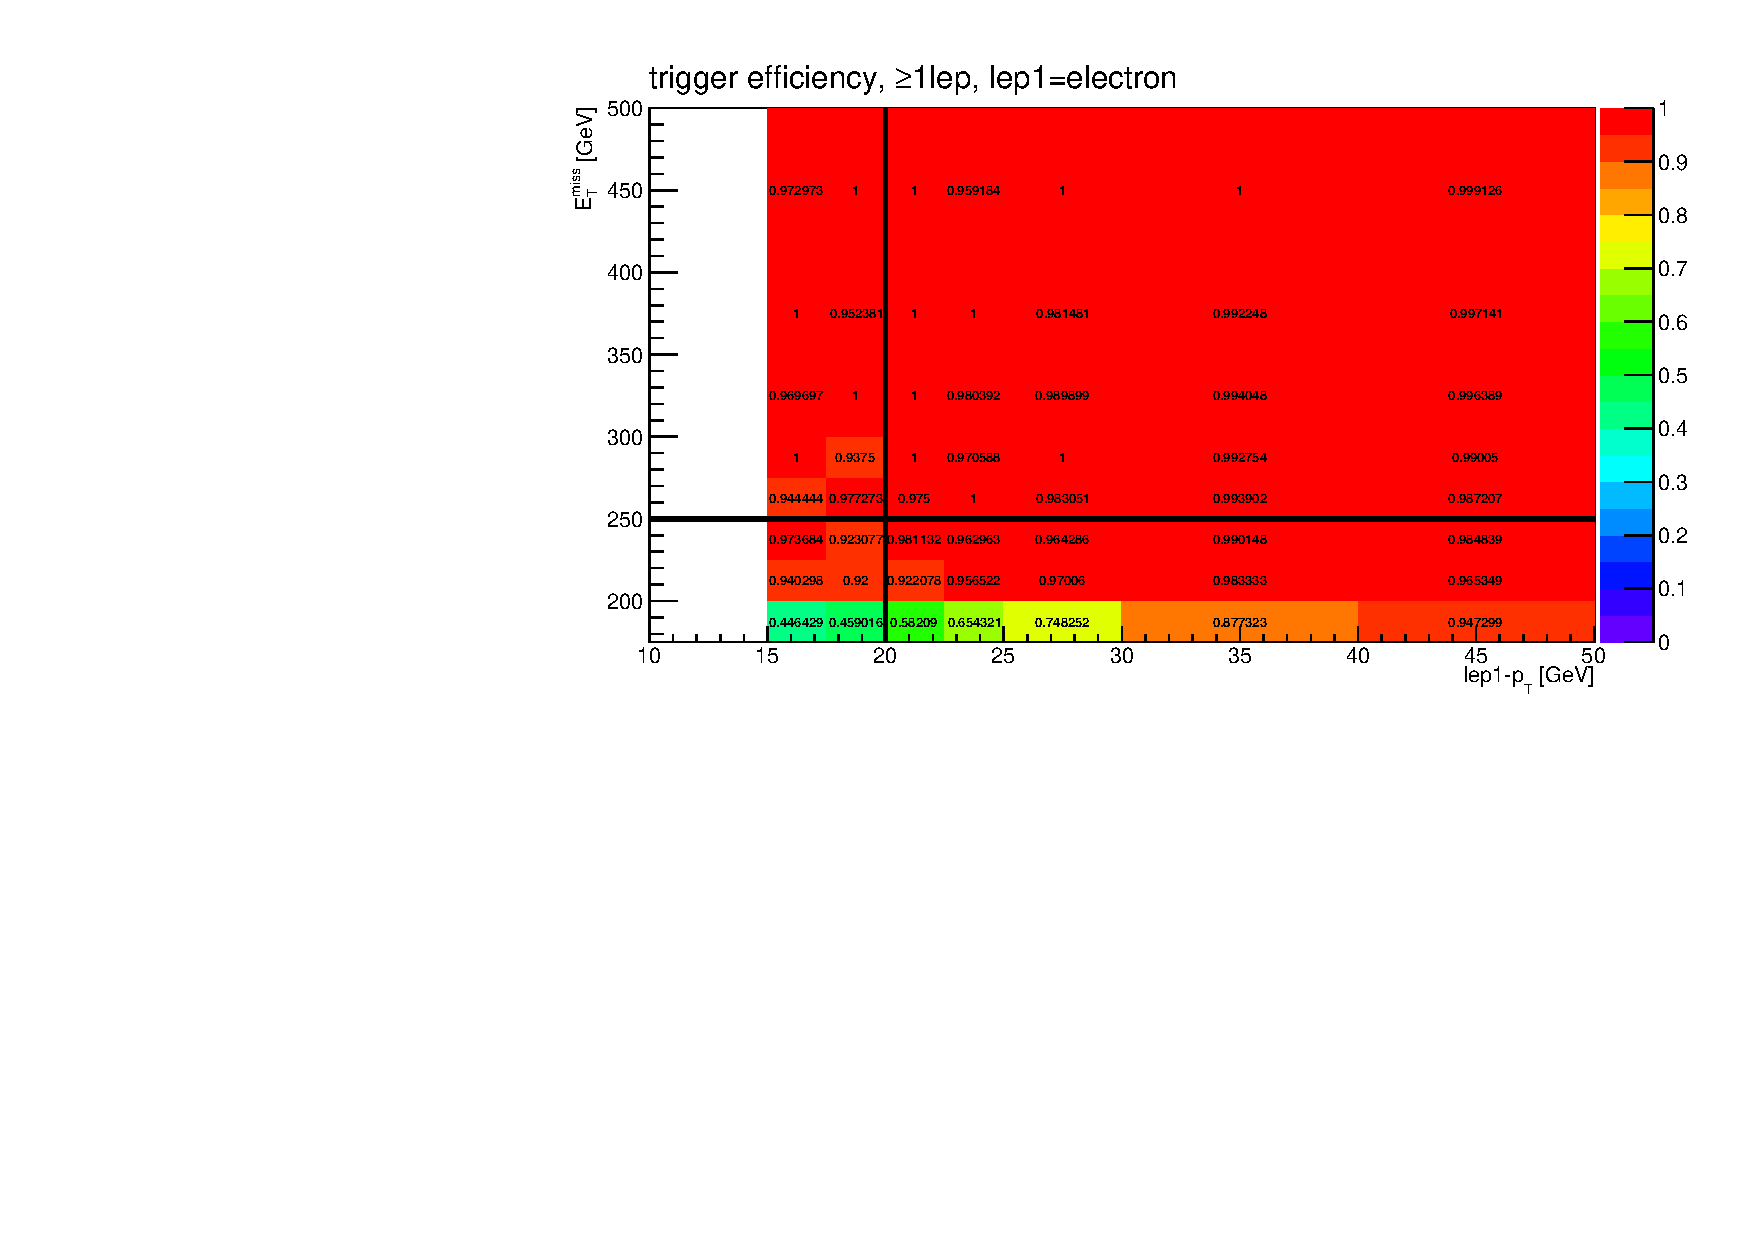
\includegraphics[width=0.45\textwidth]{figures/TriggerEff_el.pdf}
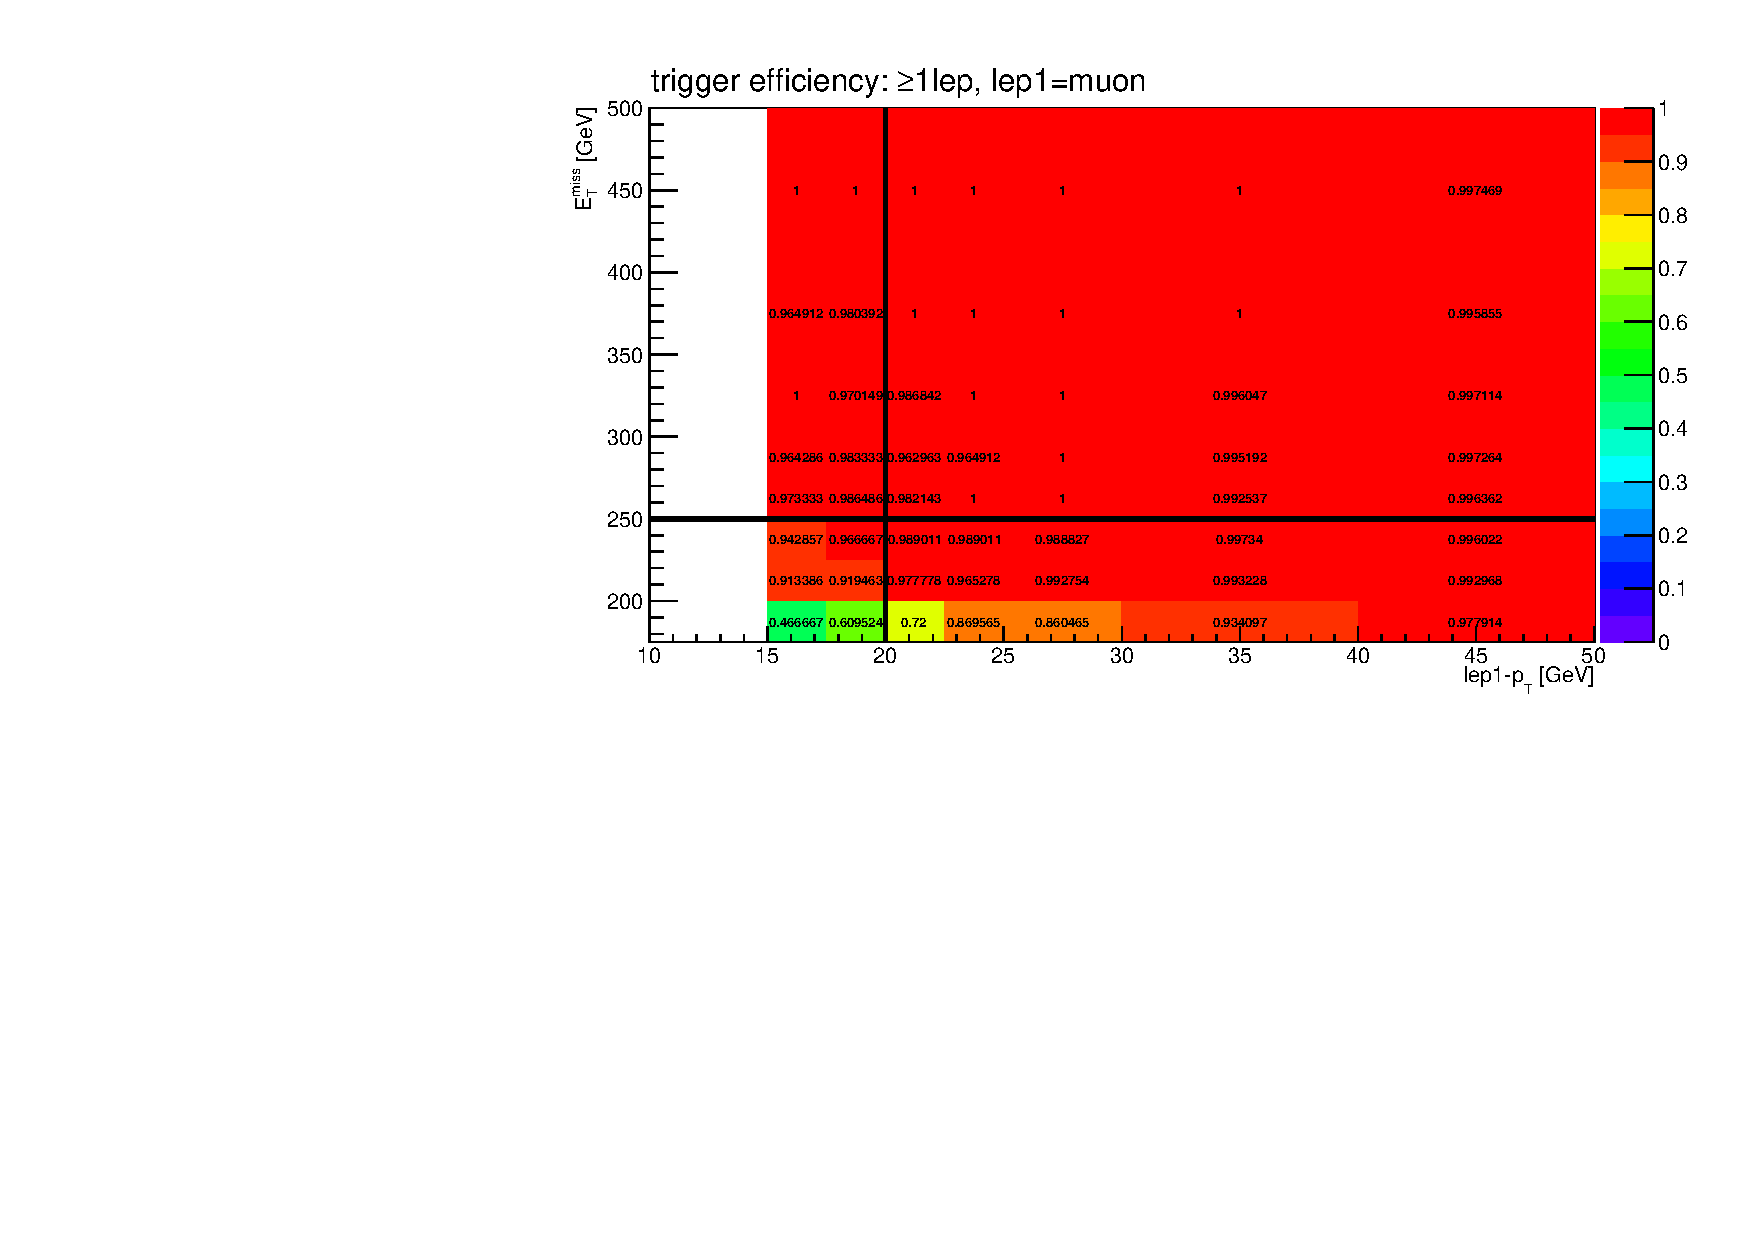
\includegraphics[width=0.45\textwidth]{figures/TriggerEff_mu.pdf}
\caption{Measured efficiencies for the union of the single lepton and
  $\met$ triggers. Efficiency is represented by the z-axis color scale. The
  efficiencies are presented separately for the case where the leading
  lepton is an electron (left), and a muon (right).}
\label{fig:stop:trigeff:1lepmet}
\end{figure}

As Section \ref{ssec:stop:lostlep} will describe, certain of our
background estimation techniques compel us to treat the $p_T$ of a
second lepton as part of the $\met$. For this special case, we must
re-evaluate the efficiency of our combined single lepton and $\met$
triggers. We do so using the exact same procedures described above,
except that we additionally require events to have a second lepton
with $p_T >$ 10 GeV. These efficiencies are presented in Figure
\ref{fig:stop:trigeff:2ndlepplusmet}. Because the combined triggers
have substantial inefficiency at low $\met$ and low lepton $p_T$, we
do correct our Monte Carlo simulations for these trigger
efficiencies when performing this background estimation.

% Plots of 2nd-lep-plus-met trigger efficiency taken from AN-16-463. Unpublished!
\begin{figure}[htb]
\centering
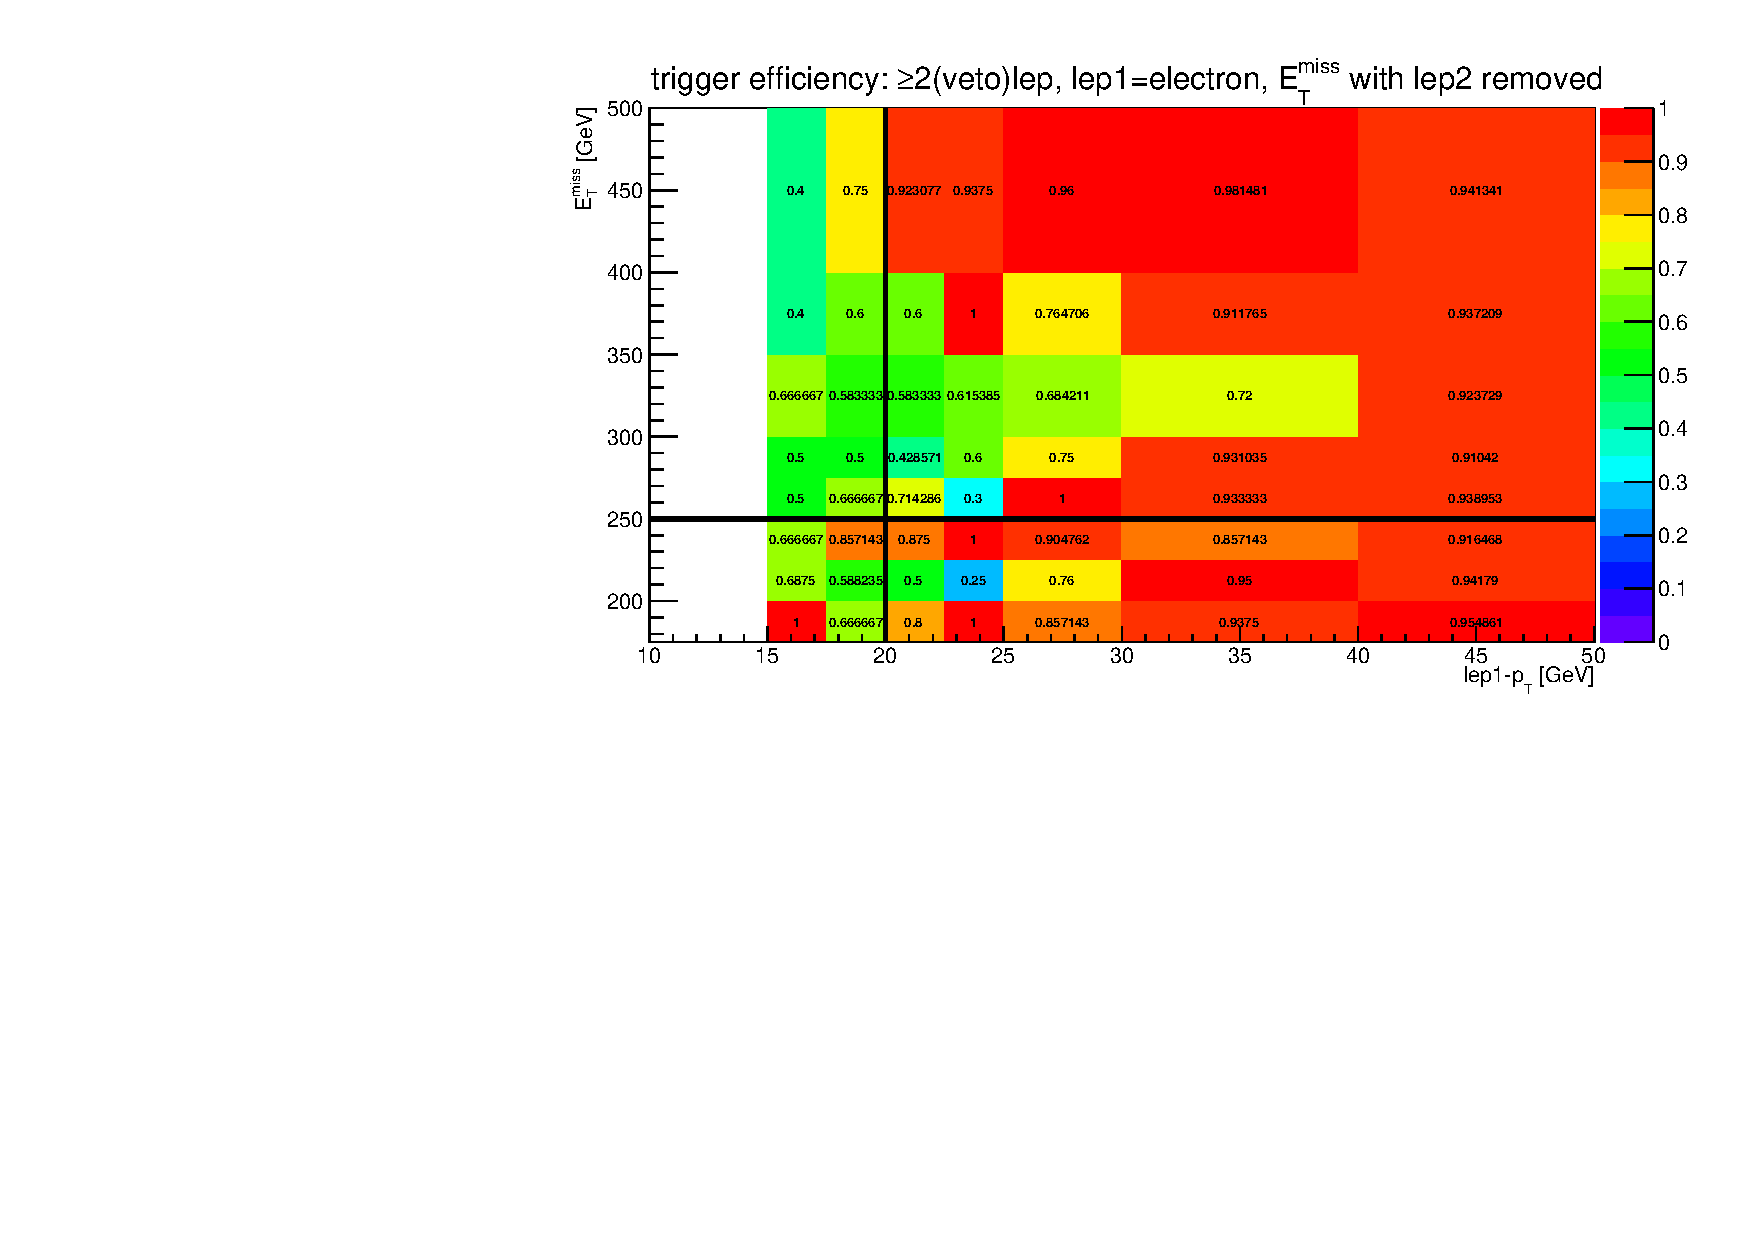
\includegraphics[width=0.45\textwidth]{figures/TriggerEff2l_el.pdf}
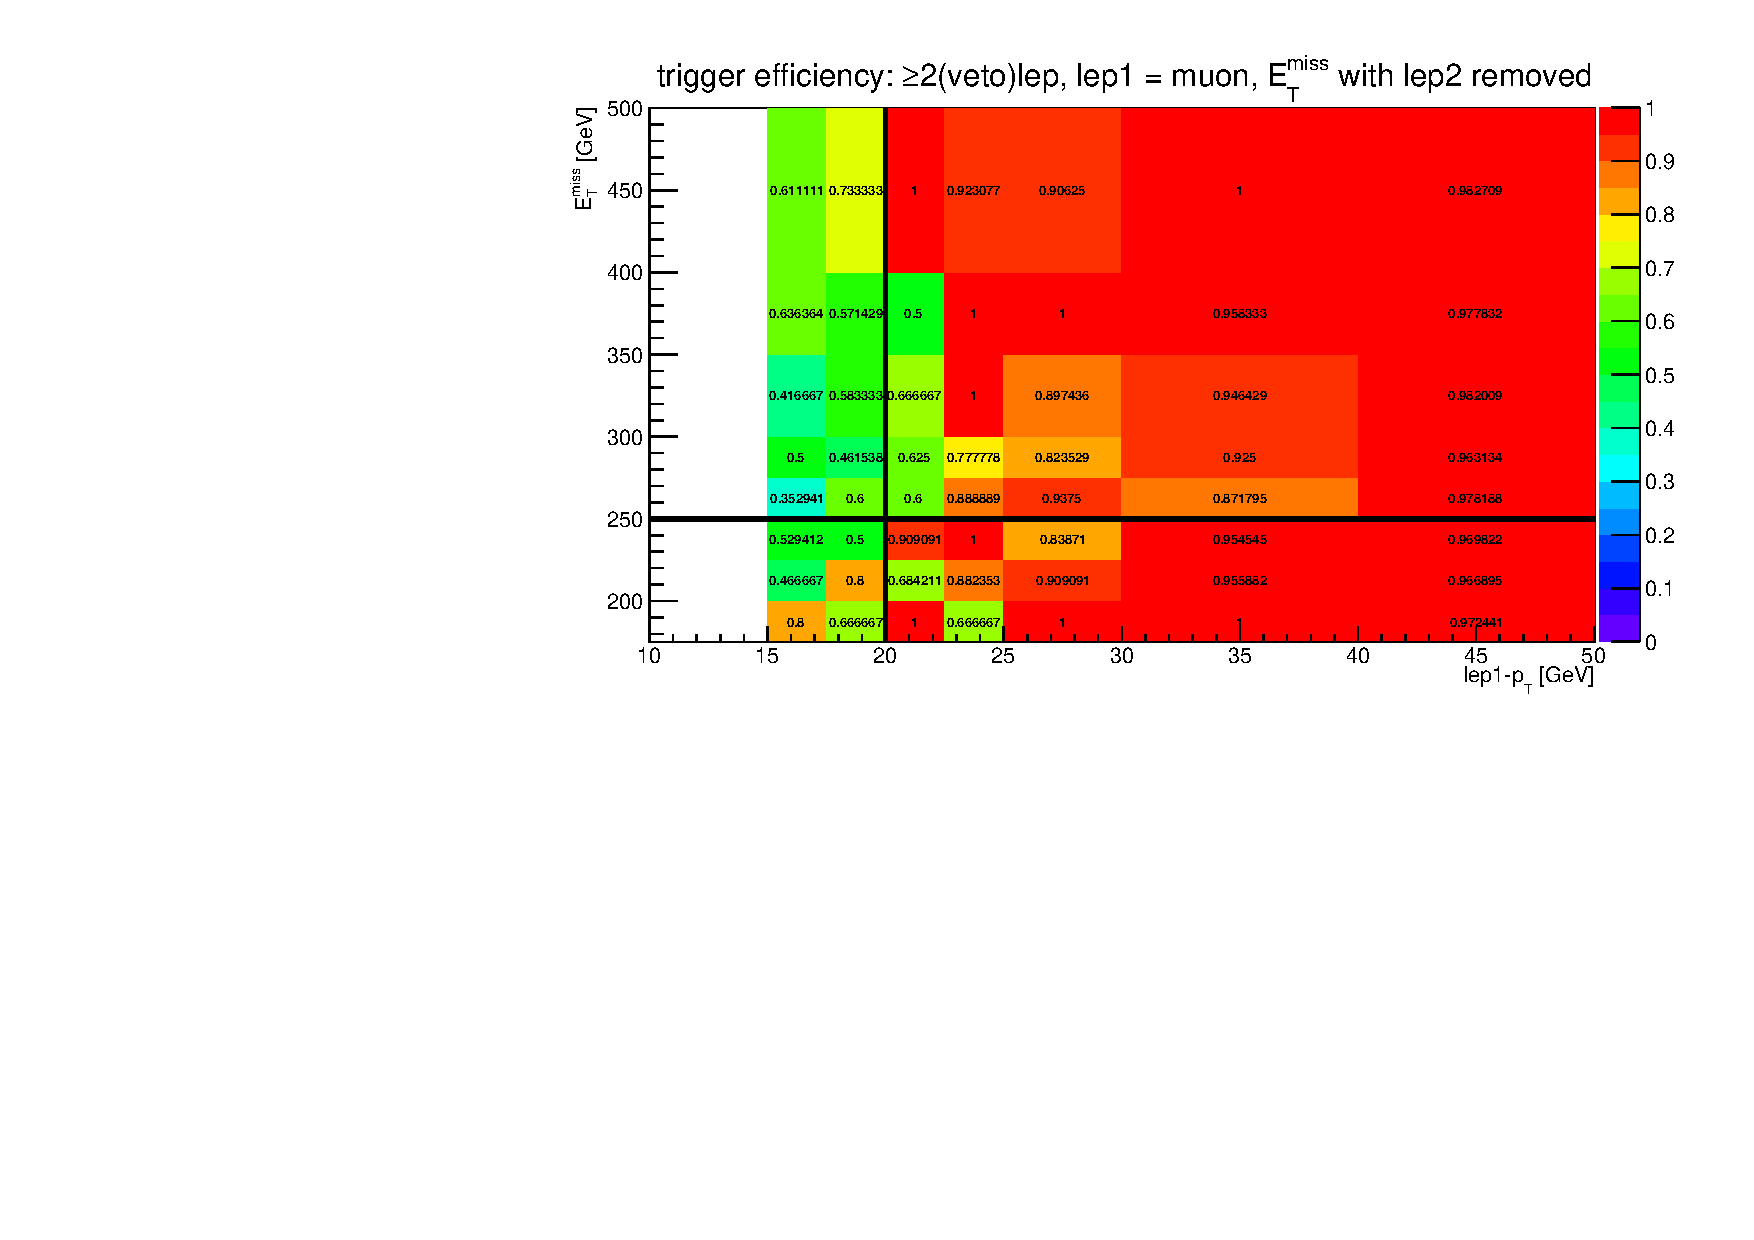
\includegraphics[width=0.45\textwidth]{figures/TriggerEff2l_mu.pdf}
\caption{Measured efficiencies for the union of the single lepton and
  $\met$ triggers, when the subleading lepton $p_T$ is added to the
  $\met$. Efficiency is represented by the z-axis color scale. The
  efficiencies are presented separately for the case where
  the leading lepton is an electron (left), and a muon (right).}
\label{fig:stop:trigeff:2ndlepplusmet}
\end{figure}

% What to say about the dilepton and single photon trigger
% efficiencies? How are these evaluated? Do we present measured
% efficiencies anywhere?

\subsection{Monte Carlo samples}
\label{ssec:stop:mcsamples}

Our analysis relies on modeling a number of background and signal
processes using Monte Carlo simulation. Table \ref{tab:stop:mcsamples}
presents the complete list of Monte Carlo samples used. All samples
are produced as MINIAODSIM.

% Table of MC samples taken from AN-16-463. Unpublished.
\begin{table}[htp]
\caption[Monte Carlo simulation datasets used in this analysis, and
  their theoretical cross sections. The symbols * and $\dagger$ replace
  longer strings.]
  {Monte Carlo simulation datasets used in this analysis, and their
  theoretical cross sections. The symbol * replaces the string
  RunIISummer16MiniAODv2-PUMoriond17\_80X\_mcRun2\_asymptotic\_2016\_TrancheIV\_v6, % Warning: underfull hboxes abound here!
  and the $\dagger$ replaces
  RunIISpring16MiniAODv2-PUSpring16Fast\_80X\_mcRun2\_asymptotic\_2016\_miniAODv2\_v0.}
\label{tab:stop:mcsamples}
\centering
%\makebox[\textwidth][c]{%
{\footnotesize
\begin{tabular}{|l|c|c|c|}
\hline
Sample & Cross Section \\
& [pb] \\
\hline
/TTJets\_SingleLeptFromT\_TuneCUETP8M1\_13TeV-madgraphMLM-pythia8/*(\_ext)-v1 & 182.7 \\
/TTJets\_SingleLeptFromTbar\_TuneCUETP8M1\_13TeV-madgraphMLM-pythia8/*(\_ext)-v1 & 182.7 \\
/TTJets\_DiLept\_TuneCUETP8M1\_13TeV-madgraphMLM-pythia8/*\_ext-v1 (and *-v4) & 87.3 \\
/ST\_tW\_top\_5f\_NoFullyHadronicDecays\_13TeV-powheg\_TuneCUETP8M1/*-v1 & 19.6 \\
/ST\_tW\_antitop\_5f\_NoFullyHadronicDecays\_13TeV-powheg\_TuneCUETP8M1/*-v1 & 19.6 \\
/ST\_t-channel\_top\_4f\_leptonDecays\_13TeV-powheg-pythia8\_TuneCUETP8M1/*-v1 & 44.1 \\
/ST\_t-channel\_antitop\_4f\_leptonDecays\_13TeV-powheg-pythia8\_TuneCUETP8M1/*-v1 & 26.2 \\
/ST\_s-channel\_4f\_leptonDecays\_13TeV-amcatnlo-pythia8\_TuneCUETP8M1/*-v1 & 3.7 \\
/W1JetsToLNu\_TuneCUETP8M1\_13TeV-madgraphMLM-pythia8/*-v1 & 11782  \\
/W2JetsToLNu\_TuneCUETP8M1\_13TeV-madgraphMLM-pythia8/*-v1 & 3841 \\
/W3JetsToLNu\_TuneCUETP8M1\_13TeV-madgraphMLM-pythia8/*-v1 & 1160 \\
/W4JetsToLNu\_TuneCUETP8M1\_13TeV-madgraphMLM-pythia8/*-v1 & 600 \\
/W1JetsToLNu\_NuPt-200\_TuneCUETP8M1\_13TeV-madgraphMLM-pythia8/*-v1 & 2.36  \\
/W2JetsToLNu\_NuPt-200\_TuneCUETP8M1\_13TeV-madgraphMLM-pythia8/*-v1 & 4.95 \\
/W3JetsToLNu\_NuPt-200\_TuneCUETP8M1\_13TeV-madgraphMLM-pythia8/*-v1 & 4.94 \\
/W4JetsToLNu\_NuPt-200\_TuneCUETP8M1\_13TeV-madgraphMLM-pythia8/*-v1 & 8.83 \\
/ttWJets\_13TeV\_madgraphMLM/*-v1 & 0.61 \\
/ttZJets\_13TeV\_madgraphMLM/*-v1 & 0.78 \\
/WWTo2L2Nu\_13TeV-powheg/*-v1 & 12.18 \\
/WWToLNuQQ\_13TeV-powheg/*-v1 & 50.00  \\
/WZTo3LNu\_TuneCUETP8M1\_13TeV-powheg-pythia8/*-v1 & 4.43 \\
/WZTo2L2Q\_13TeV\_amcatnloFXFX\_madspin\_pythia8/*-v1 & 5.60 \\
/WZTo1L1Nu2Q\_13TeV\_amcatnloFXFX\_madspin\_pythia8/*-v1 & 10.74 \\
/WZTo1L3Nu\_13TeV\_amcatnloFXFX\_madspin\_pythia8/*-v1 & 3.05 \\
/ZZTo4L\_13TeV\_powheg\_pythia8/*-v1 & 1.25 \\
/ZZTo2L2Q\_13TeV\_amcatnloFXFX\_madspin\_pythia8/*-v1 & 3.22 \\
/ZZTo2L2Nu\_13TeV\_powheg\_pythia8/*-v1 & 0.56 \\
/ZZTo2Q2Nu\_13TeV\_amcatnloFXFX\_madspin\_pythia8/*-v1 & 4.73 \\
/SMS-T2tt\_mStop-150to250\_TuneCUETP8M1\_13TeV-madgraphMLM-pythia8/$\dagger$-v1 & \\
/SMS-T2tt\_mStop-250to350\_TuneCUETP8M1\_13TeV-madgraphMLM-pythia8/$\dagger$-v1 & \\
/SMS-T2tt\_mStop-350to400\_TuneCUETP8M1\_13TeV-madgraphMLM-pythia8/$\dagger$-v1 & \\
/SMS-T2tt\_mStop-400to1200\_TuneCUETP8M1\_13TeV-madgraphMLM-pythia8/$\dagger$-v1 & \\
/SMS-T2bW\_TuneCUETP8M1\_13TeV-madgraphMLM-pythia8/$\dagger$-v1 & \\
/SMS-T2bt\_TuneCUETP8M1\_13TeV-madgraphMLM-pythia8/$\dagger$-v1 & \\
\hline
\end{tabular}
}
\end{table}

\section{Search Strategy}
\label{sec:stop:searchstrategy}

Because we are searching for single lepton stop decays, we must select
events with one and only one lepton in them. In addition, the LSPs and
charginos should go undetected by the CMS detector; those sparticles
plus the neutrino should give relatively
large amounts of $\met$. Therefore, our main experimental signature is a
single lepton plus high $\met$.

Many other physics processes can produce a single lepton plus high
$\met$, or can produce signatures that resemble these. We must therefore
identify these backgrounds, and attempt to reduce their presence using
a series of cuts and selections. When it is not possible to mitigate
the backgrounds with cuts, we must attempt to estimate how many
background events fall into our signal regions so we can exclude them
from the final calculations.

In the absence of any particular cuts and selections, the largest
background will naturally be SM processes that produce one true lepton
and large $\met$. The notable example is $\ttonelep$,
though other processes contribute as well, such as W-boson production
with jets, where the W decays leptonically. In order to combat this
background component, we first add a cut on the transverse mass of the
lepton plus the $\met$, or $\mt$. The exact formula for this variable is
given by Equation \ref{eq:stop:mt} in Section \ref{ssec:stop:mt}. This cut works in
concert with our high-$\met$ requirement to help reduce the single-lepton
background component.

% Insert MT figures from AN

Figure \ref{fig:stop:mtstudies} shows the results of several
investigations into the $\mt$ variable. The left plot shows the
reconstructed value of $\mt$ in a sample of W($\ell\nu$)+jets MC
events, with three different $\met$ cuts applied. As the plot shows,
higher $\met$ requirements cause the W-boson mass edge to become more
sharply defined. % So? What does this really tell us?

The center plot shows generator-level $\mt$ and reconstructed $\mt$
for both W+jets and $\ttonelep$ simulated events. These
events were selected by requiring one single lepton and at least 2
jets, all with $p_T > 30$ GeV, and $\met >$ 250 GeV. The generator-level $\mt$ was
calculated using the neutrino momentum in place of the $\met$. The plot
shows that the tails of the $\mt$ distribution look very different for
W+jets and $\ttonelep$. In the case of $\ttonelep$, the top mass
restricts the mass spectrum of the W-boson, so that most events in the
tail are simply due to the limited resolution of $\met$
reconstruction. By contrast, in W+jets events, there is no constraint
on the W mass, so the tail is attributable to the natural width of the
W-boson mass spectrum. Thus, by selecting an appropriate $\mt$ cut, we
can effectively reduce the single lepton background to mostly W+jets
events. We can then estimate the size of the remaining background
component using techniques that will be described in Sections
\ref{ssec:stop:1lw} and \ref{ssec:stop:1ltop}. % Do I need to rewrite this to be clearer?

% Does the third plot actually show us anything? Is it important to
% include it?

After reducing the single lepton background using $\met$ and $\mt$ cuts,
the next largest background comes from events with two genuine
leptons, such as $\ttdilep$, where one of the leptons is not
reconstructed. As Section \ref{sec:stop:selections} will describe, we
veto events that have a second electron, muon, or tau, as well as
events with an isolated track in them. Nevertheless, these vetos are
not perfect. And often, a second lepton falls outside our range of
acceptance in $p_T$ or $\eta$, is not isolated, or is not
reconstructed. We call this component the ``lost lepton'' background,
and estimate it using techniques described in Section
\ref{ssec:stop:lostlep}.

The final background to consider is events with one genuine lepton,
but where the high $\met$ comes from a $Z \rightarrow \nu\nu$ decay,
and not from SUSY particles. The largest contributor to this
background is TTZ events, where the $\ttbar$ pair decays
semileptonically and the Z decays to invisible neutrinos; the next
largest contributor is WZ production. There is little we can do to
exclude such events with cuts; fortunately, this background component
is relatively small. We estimate the $Z \rightarrow \nu\nu$
component using MC with theoretical uncertainties applied, as
described in Section \ref{ssec:stop:rarebkg}.

\section{Object and Event Selection}
\label{sec:stop:selections}

% Give some intro paragraph here. Something that flows nicely.

\subsection{Vertex Selections}
\label{ssec:stop:vtxselections}

For an event to be selected, at least the first vertex in the event
must be a good vertex. A vertex is considered to be ``good'' if it
meets the following criteria:

\begin{itemize}
\item The tracks used to create the vertex must have trajectory fits
  with positive $\chi^2$ values.
\item The vertex fit must have at least 5 degrees of freedom.
\item The distance between the vertex and the nominal center of the
  detector must have a $z$-component of less than 24 cm.
\item The same distance must have a transverse component, $\rho$, of
  less than 2 cm.
\end{itemize}

If multiple vertices in an event meet these criteria, we choose the
one whose associated tracks have the highest $\sum p_T^2$ to be our
primary vertex (PV), from which all of our physics objects originate.

\subsection{Lepton Selections and Veto}
\label{ssec:stop:lepselections}

We select events that have one well-identified reconstructed lepton
(electron or muon), and veto events with additional leptons. All our
identification criteria are based on the POG recommendations, and are
described in Table \ref{tab:stop:lepselections}.

For our electrons, we remove the POG-recommended isolation cut, and
substitute a cut based on \emph{relative mini-isolation}, as is standard for
SUSY searches at CMS. Relative mini-isolation is defined as the sum of
the $p_T$ of the particle flow candidates within a cone-shaped region
around the lepton, where the cone size varies with the lepton
$p_T$. For lepton $p_T <$ 50 GeV, the cone size is 0.2 in $\Delta
R$. For $p_T$ between 50 and 200 GeV, the cone size is defined to be
10.0 GeV / $p_T^{\text{lep}}$. Finally, for lepton $p_T$ above 200 GeV, the
cone size is fixed at 0.05. The rationale for reducing the cone size
as lepton $p_T$ rises is to avoid vetoing signal events
where a boosted top decays to a lepton and b-jet that are nearly
colinear. Pileup correction is performed using the average energy
density in the event, and the same effective area used in the
mini-isolation calculation.

\begin{table}[htb]
\centering
\caption{Criteria used to identify electrons or muons. We select
  exactly one good lepton, and veto any additional leptons, using two
  different sets of criteria.}
\label{tab:stop:lepselections}
\begin{tabular}{ l | l | c | c }
\hline
type & variable & selected & veto \\ \hline
\multirow{4}{*}{electron} &    $p_T$ & $>20$ GeV & $>5$ GeV \\
 &   $|\eta|$ & $<1.442$ & $<2.4$ \\
 &   POG ID without ISO & Medium & Veto \\
 &   relative miniisolation & $<0.1$ & $<0.2$ \\
 \hline
 \multirow{4}{*}{muon} &    $p_T$ & $>20$ GeV & $>5$ GeV \\
 &   $|\eta|$ & $<2.4$ & $<2.4$ \\
 &   POG ID & Medium & Loose \\
 &   relative miniisolation & $<0.1$ & $<0.2$ \\
\hline
\end{tabular}
\end{table}

\subsection{Isolated Track Veto}
\label{ssec:stop:isotrackveto}

In addition to vetoing events with a second electron/muon, we must
also reject events with a tau in them. Taus mostly decay in flight, so
to reject taus, we must reject their decay products. Some 50\% of the
time, taus decay to a charged pion or kaon. Decays to an electron and
a muon account for another 17.5\% each. Summing these cases up, we see
that 85\% of all tau decays produce a single charged track. So the
most powerful way to veto taus is to veto isolated charged
tracks. These tracks are found in the pfChargedHadrons collection. The
event is vetoed if at least one pfChargedHadron is found that meets these
criteria:
\begin{itemize}
\item $p_T >$ 10 GeV
\item $|\eta| <$ 2.4
\item Charge is opposite in sign from the selected lepton
\item $\Delta R >$ 0.4 from the selected lepton
\item $z$-component of the distance to the PV is $<$ 0.1 cm
\end{itemize}
We measure the isolation of a charged track using tracker-only
isolation, because tau decays sometimes produce multiple neutral
hadrons along with the charged track, and these hadrons should not be
counted against the track isolation. With that in mind, we require our
veto tracks to have the following isolation values:
\begin{itemize}
\item For track $p_T >$ 60 GeV, absolute tracker iso within a cone of
  0.3 must be $<$ 6 GeV.
\item For track $p_T \leq$ 60 GeV, relative tracker iso within a cone
  of 0.3 must be  $<$ 0.1.
\end{itemize}
Relative isolation is, again, isolation divided by the $p_T$ of the
object being considered. We use absolute isolation above $p_T$ of 60
GeV because relative isolation becomes a weak requirement at high
$p_T$.

\subsection{Hadronic Tau Veto}
\label{ssec:stop:hadtauveto}

Although highly effective, the isolated track veto does not address
cases where the tau decays to three charged hadrons (3-pronged
decay). So we add another veto targeting hadronic tau decays, using an
ID recipe approved by the tau POG within CMS. We veto events if we
find a hadronic tau that meets these criteria:

\begin{itemize}
\item $p_T >$ 20 GeV
\item $|\eta| <$ 2.4
\item Passes tau identification algorithm \emph{byDecayModeFinding}
\item Passes isolation selection
  \emph{byMediumCombinedIsolationDeltaBetaCorr3Hits}
\item Charge is opposite in sign from the selected lepton
\item $\Delta R >$ 0.4 from the selected lepton
\end{itemize}

\subsection{Jets}
\label{ssec:stop:jets}

We reconstruct jets using the anti-$k_t$ jet clustering algorithm
\cite{antikt} with a distance parameter of 0.4. These jets must have
$p_T >$ 30 GeV, must have $|\eta| <$ 2.4, and must pass the
established jet ID at the loose working point. The jet ID requirement
is waived for our signal MC samples, because the jet ID has some
inefficiencies in samples made using FastSim. We apply the official
CMS jet energy corrections. Each event is required to have at least
two jets; some signal regions have higher requirements to
suit their purposes, as Section \ref{sec:stop:sigregs} will describe.

We also require each event to have at least one b-tagged jet, where
b-tagging is performed using the CSVv2 algorithm. Depending on the
signal region in question, the b-tag may be required to pass the loose
WP (CSV $>$ 0.8) or the tight WP (CSV $>$ 0.935). Section
\ref{sec:stop:sigregs} will list which WP is used for each signal region.

\subsection{\texorpdfstring{$\met$}{MET}}
\label{ssec:stop:met}

As described earlier, $\metvec$ is calculated as the negative of the vector
sum of all the particle flow candidates in the event. We recalculate
the $\met$ after the jet energy corrections have been applied to the jets
in the event. We also employ the following filters, as recommended by
the JetMET group in CMS:

\begin{itemize}
\item Primary vertex filter
\item CSC beam halo filter
\item HBHE noise filter
\item HBHEiso noise filter
\item ee badSC noise filter
\item ECAL TP filter
\item Bad muon filter
\item Bad charged hadron filter
\item Bad muons filter
\item Duplicate muons filter
\end{itemize}

\subsection{Transverse Mass (\texorpdfstring{$\mt$}{MT})}
\label{ssec:stop:mt}

As alluded to in Section \ref{sec:stop:searchstrategy}, we use the
transverse mass of the lepton-$\met$ system to reduce the prevalence of
the single-lepton background, especially $\ttonelep$. By transverse
mass, we mean the solution to the relativistic equation $M^2 = E^2 -
p^2$, but using only the transverse components of the energy and
momentum of the lepton-$\met$ system. So:
\begin{equation}
\begin{split}
\mt^2 & = E_T^2 - p_T^2 \\
 & = (\met + E_\text{T}^\ell)^2 - (\vec{p}_\text{T}^\text{miss} + \vec{p}_\text{T}^\ell)^2
\end{split}
\end{equation}
Transverse energy is defined as:
\begin{equation}
E_\text{T}^2 = m^2 + p_\text{T}^2
\end{equation}
In the case of $\met$, the missing momentum and energy are the same
thing, giving us:
\begin{equation}
\mt^2 = m_\ell^2 + 2\met E_\text{T}^\ell - 2 \metvec \cdot \vec{p}_\text{T}^\ell
\end{equation}
In our case, $m_\ell$ is negligible compared to
$p_\text{T}^\ell$. This also means $E_\text{T}^\ell \approx p_\text{T}^\ell$.
So if $\phi$ denotes the transverse angle between $\metvec$ and
$\vec{p}_\text{T}^\ell$, then we find:
\begin{equation}
\label{eq:stop:mt}
\mt = \sqrt{2 \met p_\text{T}^\ell (1 - \cos \phi)}
\end{equation}

In events with an on-shell W-boson decaying to a single lepton and no
other sources of $\met$, the largest possible value $\mt$ can take on
is the W-boson mass, around 80 GeV. Thus, by cutting on $\mt$, we can
strongly reduce the presence of $ttonelep$, W+jets, and single-top
events. This fact is illustrated in Figure
\ref{fig:stop:mt:nminusone}. As described in Section
\ref{sec:stop:searchstrategy}, background events in the tail of the
$\mt$ distribution are mostly due to off-shell W-bosons and $\met$
resolution effects.

% MT n-1 plot, taken from AN-16-463. Believed unpublished.
\begin{figure}[htb]
\centering
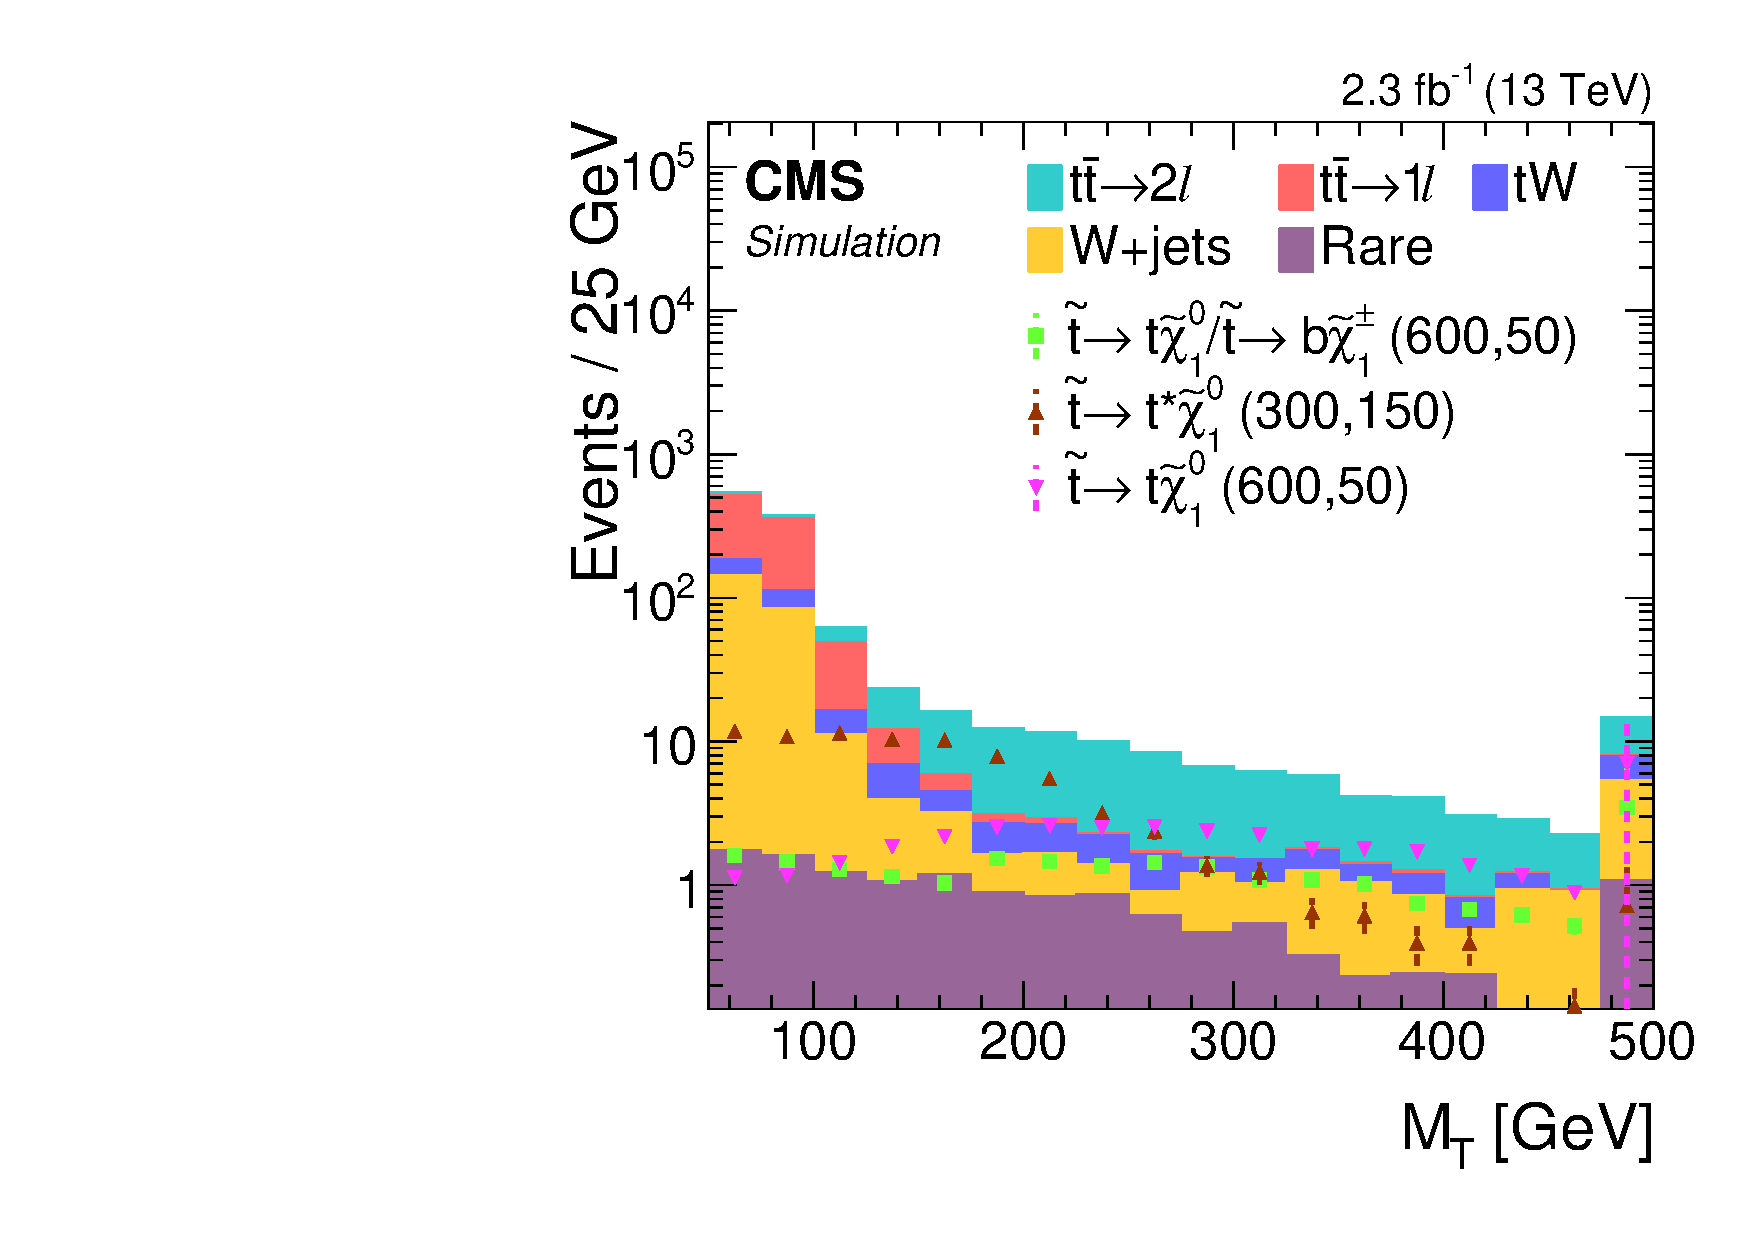
\includegraphics[width=0.6\textwidth]{figures/nminusone_mt.pdf}
\caption{Distribution of $\mt$ after all other selections have been applied.}
\label{fig:stop:mt:nminusone}
\end{figure}

\subsection{Modified Topness (\texorpdfstring{$t_{\text{mod}}$}{tmod})}
\label{ssec:stop:tmod}

In a previous search for stop quarks, particle physicists developed a
variable they called \emph{topness}, denoted $t$. This complicated
variable attempts to quantify the degree to which an event is
consistent with being a $\ttdilep$ event \cite{topness}. Although our
analysis must also suppress the $\ttdilep$ background, our
investigations showed that we could achieve better discrimination
between signal and $\ttdilep$ by removing two of the terms in the
topness variable (specifically, the center-of-mass constraint, and the
$\chi^2$ for leptonic top decay). We thus arrive at a variable we call
\emph{modified topness}, or $t_\text{mod}$. To calculate this
variable, we must minimize an expression that constrains the
neutrino-lepton system to have a mass similar to the W-boson mass, and the
b-quark-W-boson system to have a mass similar to top quark mass. Thus
we define:
\begin{equation}
\label{eq:stop:tmod}
\begin{split}
t_\text{mod} & = \ln ( \text{min} \; S ), \; \text{where} \\
S(\vec{p}_W, p_{\nu,z}) & = \frac{(m_W^2-(p_\nu+p_\ell)^2)^2}{a_W^4} + \frac{(m_t^2 - (p_{b_2}+p_W)^2)^2}{a_t^4}
\end{split}
\end{equation}

The parameters $a_W$ and $a_t$ provide the scale for the W-boson
and top quark masses; we set them to 5 GeV and 15 GeV, respectively.
There is some abiguity as to which jets should be used in this
calculation. We found that $t_\text{mod}$ behaved best across signal
models with both low and high mass splittings if we chose our jets
according to these rules:
\begin{itemize}
\item Consider all combinations of the three jets with the highest
  CSVv2 discriminator values. If at least one such jet is b-tagged,
  only consider permutations that include at least one b-tagged jet.
\item Choose the combination of jets that minimizes the ultimate
  $t_\text{mod}$ value.
\end{itemize}
Ultimately, modified topness is effective in discriminating against
both $\ttdilep$ events and single top $tW$ events. However, it also
suppresses signal models with certain kinematics. For that reason, we
choose to bin our signal regions in $t_\text{mod}$, instead of making
a strict cut on it. Figure \ref{fig:stop:tmod} shows the distribution
of $t_\text{mod}$ for our background processes and various signal mass
points.

% Plot of t_mod taken from AN-16-463. Unpublished.
%%% ALSO: needs to have the CMS header added!
\begin{figure}
\centering
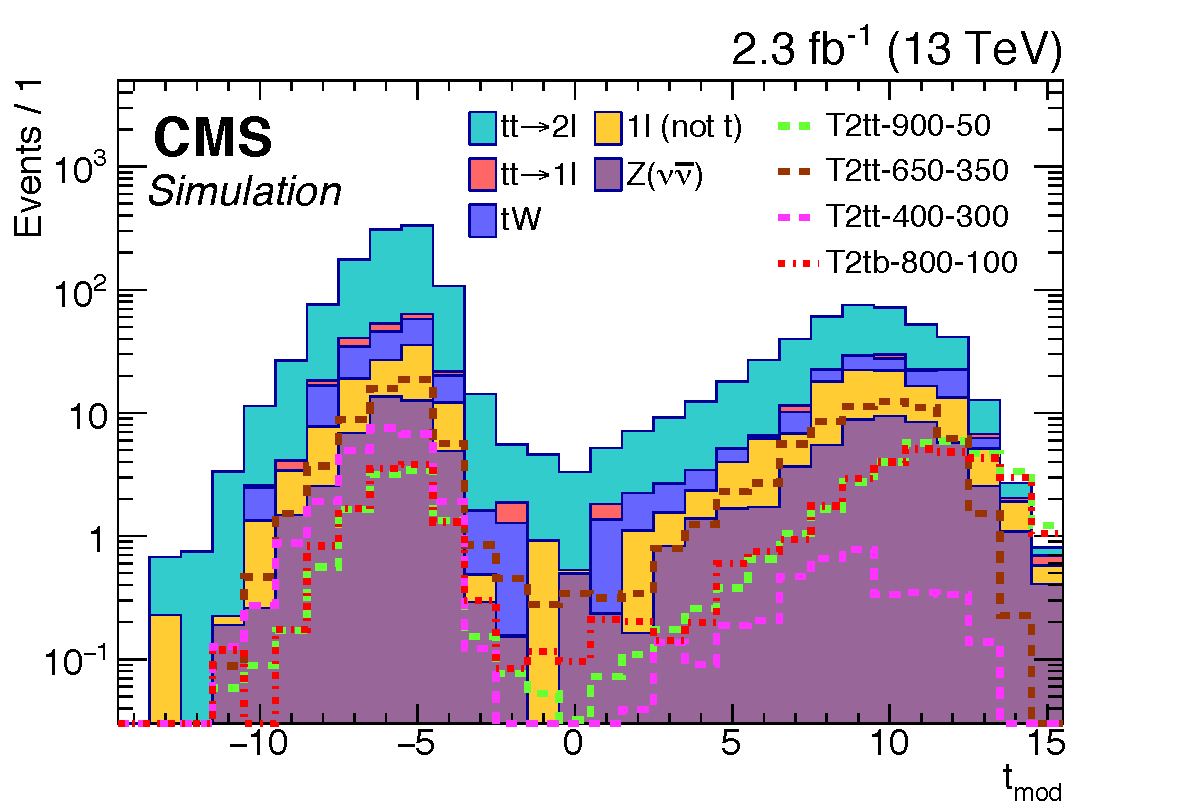
\includegraphics[width=0.6\textwidth]{figures/nminusone_tmod.pdf}
\caption{Distribution of $t_\text{mod}$ after all other selections
  have been applied. Normalization is arbitrary.}
\label{fig:stop:tmod}
\end{figure}

\subsection{Lepton-b Invariant Mass (\texorpdfstring{$M_{\ell b}$}{mlb})}
\label{ssec:stop:mlb}

Another variable that can help us discriminate signal from background
is the invariant mass of the lepton and its corresponding b-jet,
denoted $M_{\ell b}$. In the case of $\ttdilep$ and $\ttonelep$
backgrounds, as well as T2tt signals, assuming we pair our lepton with
the correct b-jet, then $M_{\ell b}$ is constrained by kinematics:
\begin{equation}
M_{\ell b} \leq \sqrt{m_t^2 - m_W^2} \approx 153 \text{GeV} % Verify this calculation for yourself!
\end{equation}
This inequality does not hold true for the W+jets background, nor for T2bW
signals. So a low-$M_{\ell b}$ requirement will reduce W+jets content
compared to the T2tt signal, and a high-$M_{\ell b}$ requirement will reduce
the $\ttbar$ backgrounds compared to the T2bW signal. As Section
\ref{sec:stop:sigregs} will describe, we use different bins of
$M_{\ell b}$ in the definitions of some of our signal regions.

We define $M_{\ell b}$ to be the invariant mass of the system of the
leading lepton and the b-tag nearest the lepton in $\Delta R$. Figure
\ref{fig:stop:mlb} shows an example distribution of this
variable. Because the W+jets background is dominant at higher
$M_{\ell b}$, and because W+jets has a much higher prevalence of
light-flavor jets over b-jets, we also tighten our b-tagging WP at
high $M_{\ell b}$.

% Mlb plot pulled from AN-16-463. Unpublished.
%%% ALSO: like plot above, needs the CMS header
\begin{figure}
\centering
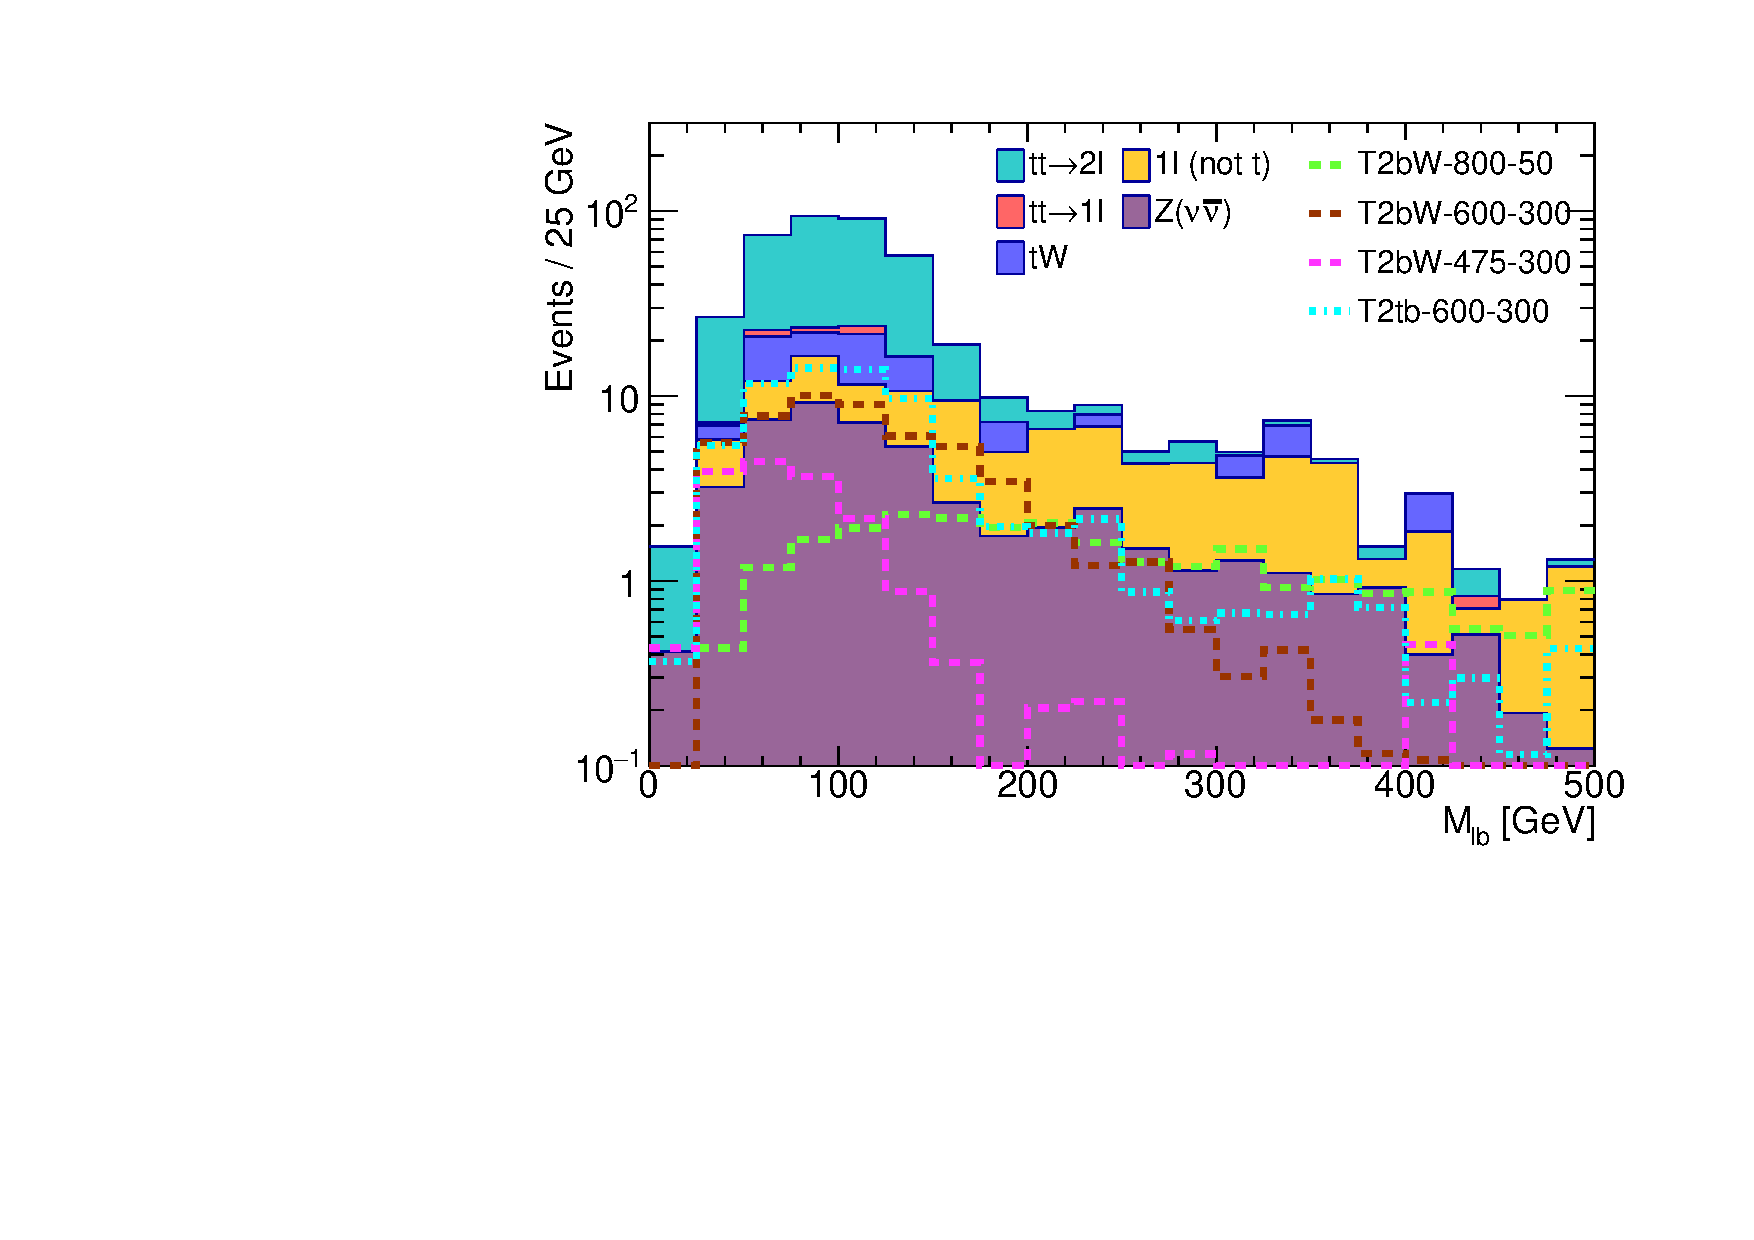
\includegraphics[width=0.6\textwidth]{figures/nminusone_mlb.pdf}
\caption{Distribution of $M_{\ell b}$ variable after baseline
  selections, in the region $t_\text{mod} > 0$. Normalization is arbitrary.}
\label{fig:stop:mlb}
\end{figure}

\subsection{Minimum Delta-Phi (\texorpdfstring{$\text{min}\Delta\phi(j_{1,2},\metvec)$}{minDphi})}
\label{ssec:stop:mindphi}

The final variable we consider in selecting our events is the minimum
$\Delta\phi$ between the $\metvec$ and either of the two leading
jets. In other words:
\begin{equation}
\text{min} \Delta\phi (j_{1,2},\metvec) = \text{min} \left\{ \Delta\phi
    (\metvec, j_1),\; \Delta\phi (\metvec, j_2) \right\}
\end{equation}
This variable allows us to reduce backgrounds such as $\ttdilep$ and
$\ttonelep$  with relatively little loss of signal, because in these
backgrounds we expect the neutrino (i.e. the source of the $\met$) to
be relatively close to the high-$p_T$ quark produced in the top
decay. Figure \ref{fig:stop:mindphi} shows the distribution of this
variable. We require a min$\Delta\phi >$ 0.8 for our bulk signal
regions; for the compressed T2tt search, this requirement is relaxed
to min$\Delta\phi >$ 0.5.

\begin{figure}
\centering
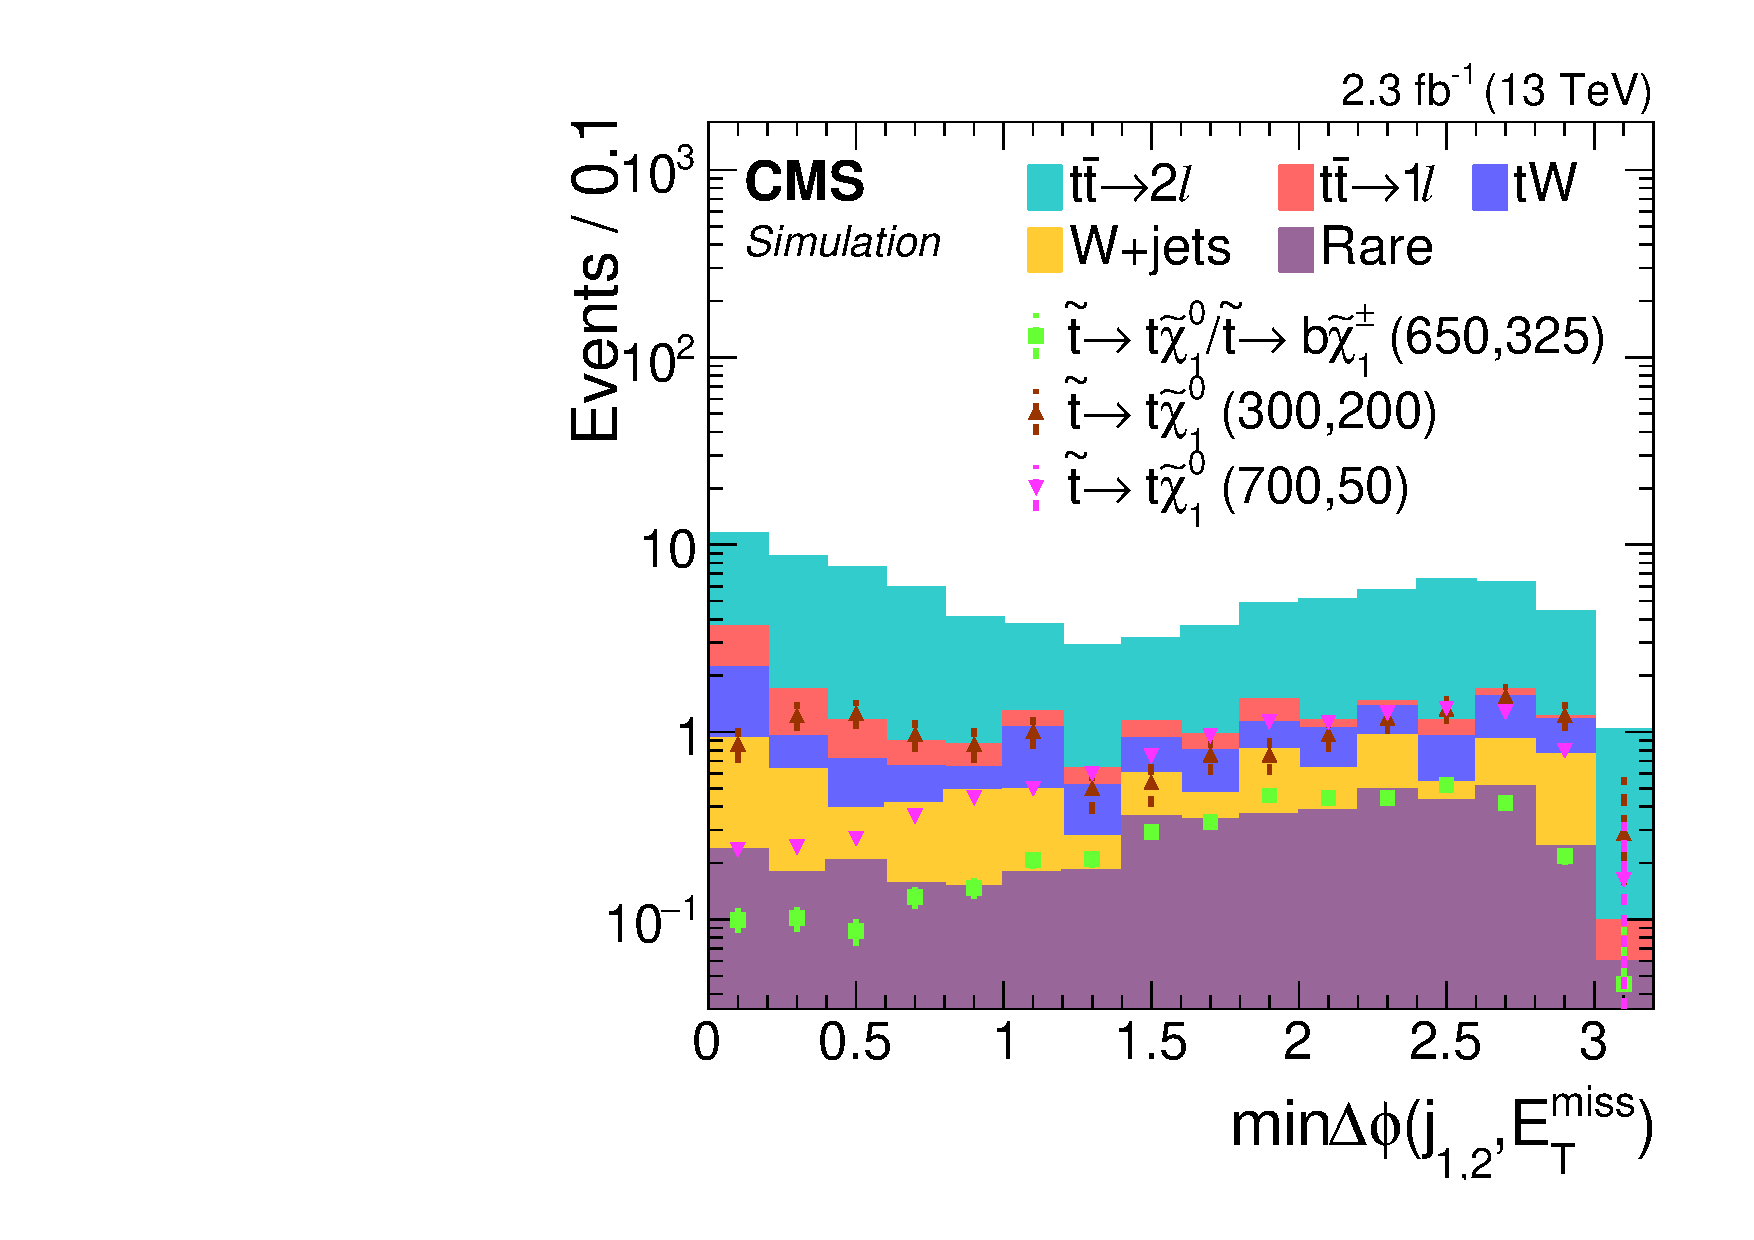
\includegraphics[width=0.6\textwidth]{figures/nminusone_mindphi.pdf}
\caption{Distribution of min$\Delta\phi (j_{1,2}, \metvec)$ after all
  other selections have been applied.}
\label{fig:stop:mindphi}
\end{figure}

\subsection{Corrections}
\label{ssec:stop:corrections}

Our Monte Carlo simulations seldom reproduce the aggregate properties of
real data with perfect accuracy. Therefore, we must reweight our
simulated events to reproduce the properties of the data more
exactly. The nominal weights applied to our MC simulations are
described here. Sections \ref{sec:stop:bkgest} and
\ref{sec:stop:signal} will describe the systematic uncertainties
on these and other weights, and how we propagate those uncertainties
to our final results.

\begin{itemize}
\item As was described in Section \ref{ssec:stop:trigeff}, we evaluate
  the efficiencies of all triggers used in this analysis. For our
  signal regions, the combined trigger efficiency is so near 100\% that we
  do not reweight our MC; in the regions where we use dilepton
  triggers, we do apply a weight for the efficiency of those triggers.
\item We apply the official jet energy corrections, as mentioned in
  Sections \ref{ssec:stop:jets} and \ref{ssec:stop:met}.
\item We apply weights to mimic the efficiency of our b-tagging
  algorithms. These weights are provided by the b-tagging POG within
  CMS. There are separate weights for heavy flavor (HF) and light
  flavor (LF) jets, as well as for the medium and tight WPs used in
  the analysis.
\item We apply weights for the efficiency of lepton identification and
  isolation, as provided by the SUSY group in CMS. We also account for
  the efficiency of vetoing a second lepton where applicable. Separate
  weights must be applied to our signal samples because they were
  generated using FastSim.
%\item % Tau and IsoTrack SFs?? % Not sure I fully understand this
% Top pT reweighting % I believe this was deprecated in favor of ttbar system pT
\item All of our signal and control regions involve binning in
  $\met$. If the $\met$ resolution differs between data and MC, we run
  the risk of MC events being counted in the wrong bin. We performed a
  separate study to measure the $\met$ resolution, % Describe this in an appendix?
  and the results are used to reweight our simulated events. Because
  the $\met$ resolution differs between the nominal and
  compressed-T2tt regions, we calculate separate weights for each. % Would be nice to be able to reference overlapping nature of these regions
\item Similar to the case of $\met$ resolution, there is a difference
  between data and MC in the $\met$ spectrum of $\ttbar$ and tW events.
  % Studied in the ttbar e/mu crosscheck region. Describe this study in an appendix.
  For simulated $\ttbar$ and tW events, we apply a weight to correct
  for this effect.
\item Initial state radiation (ISR) refers to any jets that may be
  produced alongside the main process in an event. ISR is not
  necessarily modeled correctly in our signal samples. Therefore, in
  those samples only, we reweight the events to obtain a more accurate
  distribution of the number of jets per event.
\item To correct for discrepancies in the pileup distribution, we
  reweight events using the official corrections prescribed by CMS.
% HJ will know more about the PU corrections, since he committed the
% necessary files to our repo. But since it's a CMS thing, I may not
% even need to say more.
\end{itemize}

\section{Signal Regions}
\label{sec:stop:sigregs}

As Section \ref{sec:stop:selections} has described, we preselect events
for our search using the following criteria:
\begin{itemize}
\item The first vertex must meet certain quality criteria.
\item The event must have one well-reconstructed electron or
  muon. There must be no other electrons or muons in the event, even
  of low reconstruction quality.
\item The event must not have a tau in it, or an isolated track that
  could be a tau.
\item The event must have at least two jets, of which at least one
  must be b-tagged.
\item The $\met$ must be at least 250 GeV.
\item The $\mt$ must be at least 150 GeV.
\item The minimum $\Delta \phi$ betwee the $\met$ and the two leading
  jets must be at least 0.8; at least 0.5 for the corridor search.
\end{itemize}
After those criteria have been met, events are further subdivided
among several different signal regions, to increase our sensitivity to
a wide variety of SUSY scenarios.

\subsubsection*{Nominal Signal Regions}

Our nominal signal regions are tailored to the search for most T2tt
signals, the T2bW signals, and the T2tb signals. To that end, our
signal regions are divided by the number of jets in the event, the
modified topness variable, the lepton-b-jet invariant mass, and the
amount of $\met$. These signal regions are enumerated in Table
\ref{tab:stop:nominalsrs}. At times we will refer to these regions using a
letter for the series and a number for the specific $\met$ bin, as
A3, D1, G4, etc.

% Table of nominal SRs adapted from AN-16-463. Published.
\begin{table}[htb]
\centering
\caption{Definitions of the signal regions used in the nominal search.}
\label{tab:stop:nominalsrs}
\begin{tabular}{|c|c|r|r|lllll|}
\hline
Label & $N_J$ & $t_\text{mod}$ & $M_{\ell b}$ [GeV] & \multicolumn{5}{c|}{$\met$ [GeV]} \\
\hline
A & 2-3     & $>10$ & $\leq175$     & 250-350 & 350-450 & 450-600 & $>600$ & \\
B & 2-3     & $>10$ & $>175$        & 250-450 & 450-600 & $>600$ & & \\
C & $\geq4$ & $\leq0$ & $\leq175$   & 250-350 & 350-450 & 450-550 & 550-650 & $>650$ \\
D & $\geq4$ & $\leq0$ & $>175$      & 250-350 & 350-450 & 450-550 & $>550$ & \\
E & $\geq4$ & 0-10 & $\leq175$      & 250-350 & 350-550 & $>550$ & & \\
F & $\geq4$ & 0-10 & $>175$         & 250-450 & $>450$ & & & \\
G & $\geq4$ & $>10$ & $\leq175$     & 250-350 & 350-450 & 450-600 & $>600$ & \\
H & $\geq4$ & $>10$ & $>175$        & 250-450 & $>450$ & & & \\
\hline
\end{tabular}
\end{table}

The signal regions that require 2-3 jets and $t_\text{mod} >$ 10
(the A and B series) are
designed to target T2tb signals. Because we take the mass difference
between the chargino and the LSP to be only 5 GeV in this model, the
W-boson produced in the chargino to LSP decay will be very off
shell. Thus the lepton will come from the top decay, and the off-shell
W will decay into very weak jets that we cannot resolve. In addition,
these regions will also have sensitivity to any of our signal models
where the stops are highly boosted and cause two jets to merge into one.

The remaining nominal signal regions (C-H) target T2tt and T2bW
models. They include a four jet requirement because we expect two b-jets from the
top or stop decays and two more jets from the hadronic W decay.

The three bins in $t_\text{mod}$ are formulated to enhance three different
types of signal kinematics against the $\ttdilep$
background. As Figure \ref{fig:stop:tmod} shows, the compressed
case, where the mass splitting
between the stop and the LSP is small, is most prominent when
$t_\text{mod}$ is $<$ 0. When $0 < t_\text{mod} < 10$, signal models % Rewrite when able?
with moderate mass splittings will stand out most against
$\ttdilep$. And when $t_\text{mod} >$ 10, the $\ttdilep$ background
drops off substantially faster than signals with a large mass
splitting.

The binning in $M_{\ell b}$ follows from the facts explained in
Section \ref{ssec:stop:mlb}. At low $M_{\ell b}$, the W+jets
background is reduced with little loss in the T2tt signal, and at high
$M_{\ell b}$, the $\ttbar$ backgrounds are reduced for little loss in
the T2bW signal. Because this reduction in $\ttbar$ leaves W+jets as
the dominant background, we also require that our one b-tag pass a
tight WP in the in the high $M_{\ell b}$ regions.

Finally, the higher the mass splitting, the more $\met$ we generally
expect in an event. So binning in $\met$ increases the
likelihood that any one particular signal model will stand out against the
SM background. We choose how many $\met$ bins to use in each series,
and where their boundaries should be, in order to give reasonable
statistics in all signal regions.

\subsubsection*{Corridor Signal Regions}

As Section \ref{ssec:stop:sigcompressed} described, previous stop
searches have struggled to achieve sensitivity in the top corridor
region because compressed T2tt decays are suppressed and difficult to
detect. In order to address this deficit, I developed a dedicated
search strategy focused on increasing our acceptance of compressed
T2tt signals, while maintaining a low rate of SM background
events. The final product of my work was four additional signal
regions to add to our overall search strategy.
% Would be nice to mention that I validated that it worked with all
% our background estimation techniques, etc.

The dedicated corridor signal regions use the same event selections as
the nominal signal regions, except for the following changes:
\begin{itemize}
\item I require at least 5 jets in the event.
\item The highest-$p_T$ jet must not be b-tagged using the medium WP.
\item The $p_T$ of the lepton in the event must be $<$ 150 GeV.
\item The azimuthal angle between the $\met$ and the lepton, $\Delta
  \phi (\met, \ell)$, must be $<$ 2.0.
\item As described earlier, the min$\Delta \phi(j_{1,2},\metvec)$
  must be $>$ 0.5.
\end{itemize}
In addition to these selections, the four corridor signal regions are
defined by four bins in $\met$, given by Table \ref{tab:stop:corridorsrs}:

% Table of corridor SR met bins, adapted from AN-16-463. Something like this is published.
\begin{table}[h]
\centering
\caption{$\met$ bins used in the dedicated corridor signal regions.}
\label{tab:stop:corridorsrs}
\begin{tabular}{|c|cccc|}
\hline
Label & \multicolumn{4}{c|}{$\met$ [GeV]} \\
\hline
I & 250-350 & 350-450 & 450-550 & $>550$ \\
\hline
\end{tabular}
\end{table}

To develop these signal regions, I considered the unique kinematics of
compressed T2tt signals, and how they might affect the variables
already employed in our stop search. I also considered whether any new
variables might be able to discriminate compressed T2tt from the SM
background. Although several variables had the potential to
discriminate compressed T2tt from background, I made the final choice
by measuring which added cuts provided the greatest increases in
expected sensitivity, measured using a simplified version of the
limit-setting procedure described later in Section
\ref{sec:stop:interp}.

Compressed stop decays, by virtue of their off-shell top quark, tend
to have lower $\met$ than the bulk signals. So one of the first
modifications I considered was relaxing our $\met$
requirement. However, I found that any reduction in $\met$ would cause a
proportionally larger increase in background yield than in signal
yield. With the 250 GeV $\met$ cut firmly fixed in place, we then
asked how might a compressed stop decay generate such large $\met$?
The answer to that question ultimately became the defining element of
the corridor search strategy.

We concluded that in the corridor region, in order to generate at least
250 GeV of $\met$, a stop pair must have a large boost. Momentum conservation
dictates that in order to have a large boost, the stop pair should be
recoiling off some other physics object. The most likely candidate was
a high-$p_T$ jet produced as ISR. Because we expected another jet in
the event, in addition to the four from stop decay, we imposed the
$N_J > 5$ requirement. Additionally, ISR jets seldom originate from
b-quarks, because b-quarks are fairly heavy, and thus hard to
produce. So we further target the compressed signal by requiring
that the leading jet not be b-tagged.

The $\met$ in a stop decay comes from the two LSPs, as well as the
neutrino produced alongside the single lepton. In the case where the
stop squarks are boosted, we expect the products of the stop decays,
including the main contributors to the
$\met$, to continue in the rough direction of their parents too. Thus the cut
$\Delta\phi (\met, \ell) < 2$ selects events where the lepton and the
$\met$ are not separated by a large angle. Similarly, by relaxing
the cut on min$\Delta \phi(j_{1,2},\metvec)$ to $>$ 0.5, we allow jets
produced in the stop decays to be more colinear with the lepton.
Finally, the upper bound on the lepton $p_T$ is because compressed top
quarks have less momentum to pass on to their decay products.

% Should add the four N-1 plots here, to show why we cut on these variables

It is worth noting that the dedicated corridor signal regions are not
orthogonal to the nominal signal regions. In fact, if not for the
relaxed min$\Delta\phi$ cut, the corridor signal regions would
constitute a strict subset of the nominal signal regions. To avoid
double-counting events in multiple signal regions, we decided to use
the corridor and nominal signal regions in non-overlapping regions of
phase space. Using the limit-setting machinery described in Section
\ref{sec:stop:interp}, I calculated the expected sensitivity to T2tt
signals for both the nominal and corridor signal regions at a variety
of mass points. The sensitivity is expressed as a number, $r$, the
smallest value by which one could scale the signal cross section and
be able to exclude the signal hypothesis. Put simply, lower values
of $r$ indicate greater sensitivity to the signal. In Figure
\ref{fig:stop:rratio}, I plotted the ratio
$r_\text{corridor} / r_\text{nominal}$; wherever that value is less
than 1, the corridor signal regions are expected to be more sensitive
than the nominal signal regions. Unsurprisingly, the corridor search
regions have more expected sensitivity for $\Delta M$ between 100 and
225 GeV; in other words, in the area around and between the top and W
corridors. The size of the improvement in sensitivity ranges from
about 10-30\%. We therefore use only the corridor signal regions for
T2tt models with $\Delta M$ between 100 and 225 GeV, and we use only
the nominal signal regions elsewhere.

% r-ratio between corridor and nominal signal regions. Originally made
% by moi. NOT PUBLISHED!
\begin{sidewaysfigure}
\centering
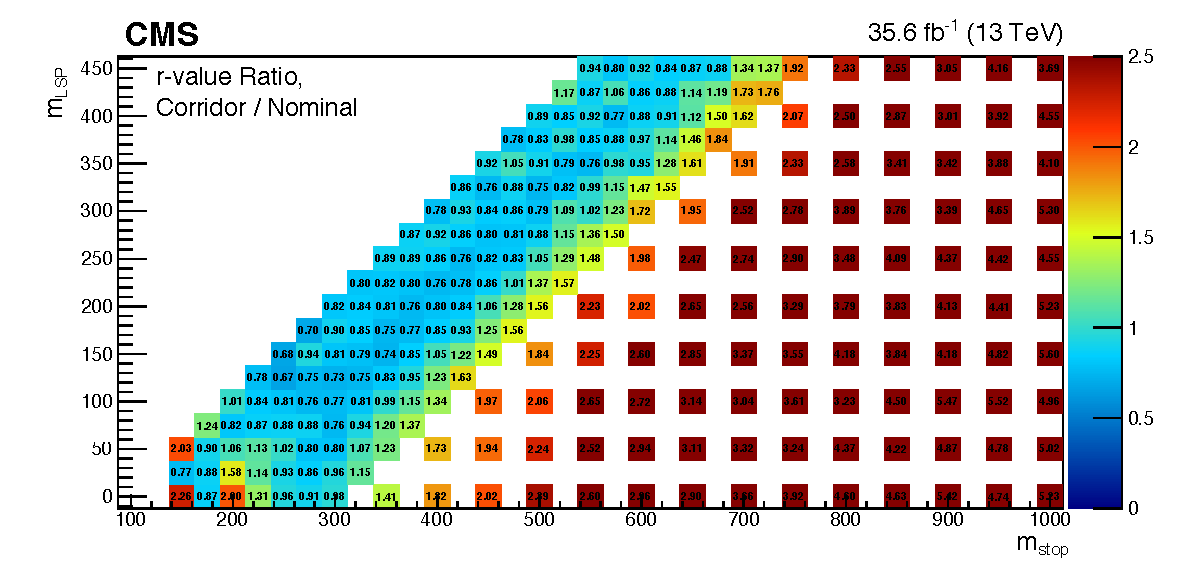
\includegraphics{figures/rratioplot.pdf}
\caption{Ratio of expected sensitivities for the corridor and nominal
  signal regions, at every mass point in the T2tt signal scan.}
\label{fig:stop:rratio}
\end{sidewaysfigure}


\section{Background Estimation}
\label{sec:stop:bkgest}

As previous sections have described, we apply a number of
preselections that reduce the prevalence of the SM backgrounds in our
search. In addition, we divide our search up into signal
regions so that we can hunt for several possible signal models while
spreading out the backgrounds. However, even with these measures,
we still expect our signal regions to be dominated by SM background
events. If we hope to find any signal from SUSY among the backgrounds,
we must be able to reliably estimate the size of the backgrounds so we
can subtract them from the measured data. We make these estimates
using a variety of techniques that will be described below. Wherever
possible, we make data-driven estimates by looking at control regions
(CRs) that are adjacent or complementary to our signal regions. In
general, the same strategies are applied to estimate backgrounds for
both the nominal and corridor signal regions. This section will also
describe how we estimate the systematic uncertainties on each
background component.

\subsection{Lost Lepton}
\label{ssec:stop:lostlep}

Across all our signal regions, the largest total background
is the lost lepton background. These are events that have two true
leptons in them, but for various reasons, the second lepton is not
caught by our second lepton veto, hadronic tau veto, or isolated track
veto. Often this loss occurs because the additional lepton is poorly
reconstructed, or falls outside the $|\eta|$ or $p_T$ ranges we can
detect. Because the second lepton is not detected, it effectively
creates additional $\met$, helping the event to pass our $\met$
requirement. Plus the additional neutrino associated with the second
lepton can help the event pass our $\mt$ cut. The dominant physics
process contributing to this background is $\ttdilep$, however there
is a strong contribution from single-top production in the $tW$
channel. Other contributors include $\ttbar$ + vector boson
production, and diboson production.

\subsubsection{Estimation Method}
\label{sssec:stop:lostlep:estimation}

We estimate the number of lost lepton events in our signal regions
based on the number of events in a set of dilepton control regions, to be
defined below. We assume that Monte Carlo simulations correctly model
the ratio of lost lepton events to dilepton events, so that the
following relationship holds true:
\begin{equation}
\label{eq:stop:lostlep:rationm}
\frac{N_{\text{lost }\ell}^\text{Data, SR}}{N_{\ell\ell}^\text{Data, CR}} =
\frac{M_{\text{lost }\ell}^\text{MC, SR}}{M_{\ell\ell}^\text{MC, CR}}
\end{equation}
In this and future equations, $N$ will denote the number of events in
actual data, and $M$ will denote the number of events in Monte Carlo
simulations.

By rearranging Equation \ref{eq:stop:lostlep:rationm}, we can derive
a data-driven estimate for the number of lost lepton events in the
signal region, using the data yield in the corresponding control region
times the SR/CR ratio derived from Monte Carlo. This ratio is known as
the lepton transfer factor, $TF_\text{lep}$. So:
\begin{equation}
\label{eq:stop:lostlep:estimate}
N_{\ell\ell}^\text{SR} = N_{\ell\ell}^\text{CR} \times \frac{M_{\ell\ell}^\text{SR}}{M_{\ell\ell}^\text{CR}}
\end{equation}

Five of the high-$\met$ CRs have very small data yields, a fact that
would contribute to large statistical uncertainty using the
extrapolaton method described above. To mitigate this uncertainty, we
combine the low-statistics bins with their neighboring bins that have
higher statistics, and add another term where we use MC to extrapolate
from the merged $\met$ bins to the single $\met$ bins:
\begin{equation}
\label{eq:stop:lostlep:metextrap}
N_{\ell\ell}^\text{SR, bin} = N_{\ell\ell}^\text{CR, merged} \times \frac{M_{\ell\ell}^\text{SR, merged}}{M_{\ell\ell}^\text{CR, merged}}
\times \left( \frac{M_{\ell\ell}^\text{SR, bin}}{M_{\ell\ell}^\text{SR, merged}} \right)
\end{equation}
The specific regions that are merged in this way are: B2/3, E2/3,
F1/2, and H1/2.

This process of extrapolating in $\met$ has the potential to introduce
errors in our measurements if the $\met$ resolution or the $\ttbar$
system properties are mismodeled in MC. In [SOME APPENDIX], we study % Appendix!
the modeling of the $\ttbar$ system using an $e/\mu$ cross-check
region, and in [SOME OTHER APPENDIX] we study the modeling of the % Appendix!
$\met$ resolution. Based on these studies, we assign appropriate scale
factors and systematic uncertainties to account for any effects due to
mismodeling. The $\met$ extrapolation also introduces some additional
uncertainty due to limited MC statistics.

\subsubsection{Control Region Definitions}
\label{sssec:stop:lostlep:crdefinitions}

To form our dilepton control regions, we use the same selections and
binning as the signal regions, except that we invert the veto on
additional leptons. Whereas the signal regions require the \textbf{absence} of
a second electron or muon, our dilepton control regions require the
\textbf{presence} of a second reconstructed electron or muon passing the
veto ID (described earlier), and with $p_T >$ 10 GeV. To simplify
our estimate and its uncertainties, we do not invert the
hadronic tau or isolated track vetos. Because lost leptons contribute
to $\met$ in our signal regions, when working with the dilepton
control regions we add the trailing lepton $p_T$ to the $\met$, and
recalculate all derived quantities that are based on $\met$. This
helps us keep the conditions as similar as possible between the CRs
and the SRs.

The data and MC yields in the dilepton control regions are given in
Table \ref{tab:stop:lostlep:cryields}. The events in the control
regions receive all the same corrections as the SR
events. The only difference is in the trigger weights, because we
select dilepton events using dilepton triggers.
Our control regions are over 95\% pure in dilepton events,
so we make no correction for impurities. The rightmost column of Table
\ref{tab:stop:lostlep:cryields} presents the ratio of the data to MC
yields. In some regions, this ratio differs considerably from
unity. Such differences in normalization between data and MC
actually have no effect on our final background estimate. Looking at Equation
\ref{eq:stop:lostlep:estimate}, we see that the background
normalization comes entirely from the CR data, and that MC is used
only to calculate the transfer factor from the CRs to SRs (and the
$\met$ extrapolation factor, where relevant).

% Dilepton CR yield table, adapted from AN-16-463. Unpublished!
\begin{sidewaystable}
\centering
{\scriptsize
\caption{Data and Monte Carlo yields in the dilepton control regions,
  based on 35.9 fb$^{-1}$ of luminosity.}
\label{tab:stop:lostlep:cryields}
\begin{tabular}{|l|c c c c c|c|c|}
\hline
Region  & $\ge2$~leptons & $1$~lepton,~from~$W$ & $1$~lepton,~from~$t$ & $Z\rightarrow\nu\nu$ & Sum Bkg. & Data & Data/MC \\*
\hline \hline
$<4$jets,~modTopness$\ge10$,~$M_{lb}<175$,~$250<MET<350$  & 215.40 $\pm$ 4.56  & 4.27 $\pm$ 2.62  & 6.49 $\pm$ 0.95  & 1.35 $\pm$ 0.06  & 227.51 $\pm$ 5.35  & 217 $\pm$ 14.73  & 0.95 $\pm$ 0.07 \\*
$<4$jets,~modTopness$\ge10$,~$M_{lb}<175$,~$350<MET<450$  & 77.88 $\pm$ 2.80  & 0.27 $\pm$ 0.13  & 2.61 $\pm$ 0.62  & 0.65 $\pm$ 0.04  & 81.40 $\pm$ 2.87  & 75 $\pm$ 8.66  & 0.92 $\pm$ 0.11 \\*
$<4$jets,~modTopness$\ge10$,~$M_{lb}<175$,~$450<MET<600$  & 25.01 $\pm$ 1.63  & 3.33 $\pm$ 3.08  & 1.37 $\pm$ 0.44  & 0.23 $\pm$ 0.03  & 29.95 $\pm$ 3.51  & 25 $\pm$ 5.00  & 0.83 $\pm$ 0.19 \\*
$<4$jets,~modTopness$\ge10$,~$M_{lb}<175$,~$MET>600$  & 6.62 $\pm$ 0.84  & 0.02 $\pm$ 0.02  & 0.47 $\pm$ 0.27  & 0.06 $\pm$ 0.01  & 7.17 $\pm$ 0.88  & 3 $\pm$ 1.73  & 0.42 $\pm$ 0.25 \\*
\hline
$<4$jets,~modTopness$\ge10$,~$M_{lb}\ge175$,~$250<MET<450$  & 9.44 $\pm$ 0.92  & 3.15 $\pm$ 2.80  & 0.88 $\pm$ 0.36  & 0.22 $\pm$ 0.02  & 13.68 $\pm$ 2.97  & 11 $\pm$ 3.32  & 0.80 $\pm$ 0.30 \\*
$<4$jets,~modTopness$\ge10$,~$M_{lb}\ge175$,~$450<MET<650$  & 2.64 $\pm$ 0.51  & 0.05 $\pm$ 0.03  & ---  & 0.04 $\pm$ 0.01  & 2.72 $\pm$ 0.51  & 3 $\pm$ 1.73  & 1.10 $\pm$ 0.67 \\*
$<4$jets,~modTopness$\ge10$,~$M_{lb}\ge175$,~$MET>600$  & 0.75 $\pm$ 0.26  & 0.05 $\pm$ 0.03  & 0.15 $\pm$ 0.15  & 0.01 $\pm$ 0.00  & 0.95 $\pm$ 0.31  & --- & --- \\*
\hline
$\ge4$jets,~modTopness$<0.0$,~$M_{lb}<175$,~$250<MET<350$  & 667.08 $\pm$ 7.32  & 0.71 $\pm$ 0.21  & 27.62 $\pm$ 1.81  & 4.87 $\pm$ 0.11  & 700.28 $\pm$ 7.54  & 675 $\pm$ 25.98  & 0.96 $\pm$ 0.04 \\*
$\ge4$jets,~modTopness$<0.0$,~$M_{lb}<175$,~$350<MET<450$  & 140.51 $\pm$ 3.45  & 2.45 $\pm$ 2.19  & 5.53 $\pm$ 0.84  & 1.28 $\pm$ 0.06  & 149.76 $\pm$ 4.17  & 150 $\pm$ 12.25  & 1.00 $\pm$ 0.09 \\*
$\ge4$jets,~modTopness$<0.0$,~$M_{lb}<175$,~$450<MET<550$  & 34.80 $\pm$ 1.75  & 0.18 $\pm$ 0.10  & 1.00 $\pm$ 0.38  & 0.33 $\pm$ 0.03  & 36.31 $\pm$ 1.79  & 27 $\pm$ 5.20  & 0.74 $\pm$ 0.15 \\*
$\ge4$jets,~modTopness$<0.0$,~$M_{lb}<175$,~$550<MET<650$  & 10.44 $\pm$ 0.95  & 0.08 $\pm$ 0.04  & 0.27 $\pm$ 0.19  & 0.13 $\pm$ 0.02  & 10.92 $\pm$ 0.97  & 7 $\pm$ 2.65  & 0.64 $\pm$ 0.25 \\*
$\ge4$jets,~modTopness$<0.0$,~$M_{lb}<175$,~$MET>650$  & 3.97 $\pm$ 0.59  & ---  & 0.14 $\pm$ 0.14  & 0.05 $\pm$ 0.01  & 4.17 $\pm$ 0.60  & 8 $\pm$ 2.83  & 1.92 $\pm$ 0.73 \\*
\hline
$\ge4$jets,~modTopness$<0.0$,~$M_{lb}\ge175$,~$250<MET<350$  & 95.64 $\pm$ 2.73  & 0.83 $\pm$ 0.24  & 5.54 $\pm$ 0.82  & 1.02 $\pm$ 0.05  & 103.03 $\pm$ 2.86  & 73 $\pm$ 8.54  & 0.71 $\pm$ 0.09 \\*
$\ge4$jets,~modTopness$<0.0$,~$M_{lb}\ge175$,~$350<MET<450$  & 25.32 $\pm$ 1.45  & 0.28 $\pm$ 0.11  & 1.39 $\pm$ 0.42  & 0.25 $\pm$ 0.03  & 27.25 $\pm$ 1.52  & 24 $\pm$ 4.90  & 0.88 $\pm$ 0.19 \\*
$\ge4$jets,~modTopness$<0.0$,~$M_{lb}\ge175$,~$450<MET<550$  & 7.16 $\pm$ 0.78  & 0.00 $\pm$ 0.00  & 0.61 $\pm$ 0.28  & 0.09 $\pm$ 0.02  & 7.86 $\pm$ 0.83  & 4 $\pm$ 2.00  & 0.51 $\pm$ 0.26 \\*
$\ge4$jets,~modTopness$<0.0$,~$M_{lb}\ge175$,~$MET>550$  & 4.92 $\pm$ 0.65  & 0.02 $\pm$ 0.02  & 0.40 $\pm$ 0.23  & 0.05 $\pm$ 0.01  & 5.38 $\pm$ 0.69  & 2 $\pm$ 1.41  & 0.37 $\pm$ 0.27 \\*
\hline
$\ge4$jets,~$0.0<$modTopness$<10$,~$M_{lb}<175$,~$250<MET<350$  & 119.79 $\pm$ 3.04  & 1.02 $\pm$ 0.74  & 12.02 $\pm$ 1.24  & 1.46 $\pm$ 0.11  & 134.29 $\pm$ 3.36  & 119 $\pm$ 10.91  & 0.89 $\pm$ 0.08 \\*
$\ge4$jets,~$0.0<$modTopness$<10$,~$M_{lb}<175$,~$350<MET<550$  & 33.87 $\pm$ 1.68  & 0.37 $\pm$ 0.14  & 4.69 $\pm$ 0.80  & 0.50 $\pm$ 0.04  & 39.42 $\pm$ 1.86  & 33 $\pm$ 5.74  & 0.84 $\pm$ 0.15 \\*
$\ge4$jets,~$0.0<$modTopness$<10$,~$M_{lb}<175$,~$MET>550$  & 1.64 $\pm$ 0.41  & 0.02 $\pm$ 0.02  & ---  & 0.05 $\pm$ 0.01  & 1.71 $\pm$ 0.42  & 1 $\pm$ 1.00  & 0.58 $\pm$ 0.60 \\*
\hline
$\ge4$jets,~$0.0<$modTopness$<10$,~$M_{lb}\ge175$,~$250<MET<450$  & 7.95 $\pm$ 0.79  & 0.53 $\pm$ 0.19  & 1.58 $\pm$ 0.44  & 0.18 $\pm$ 0.02  & 10.24 $\pm$ 0.92  & 16 $\pm$ 4.00  & 1.56 $\pm$ 0.42 \\*
$\ge4$jets,~$0.0<$modTopness$<10$,~$M_{lb}\ge175$,~$MET>450$  & 1.31 $\pm$ 0.32  & 0.15 $\pm$ 0.10  & 0.26 $\pm$ 0.18  & 0.13 $\pm$ 0.11  & 1.85 $\pm$ 0.39  & 1 $\pm$ 1.00  & 0.54 $\pm$ 0.55 \\*
\hline
$\ge4$jets,~modTopness$\ge10$,~$M_{lb}<175$,~$250<MET<350$  & 23.14 $\pm$ 1.35  & 0.13 $\pm$ 0.11  & 7.34 $\pm$ 0.95  & 0.44 $\pm$ 0.03  & 31.04 $\pm$ 1.65  & 29 $\pm$ 5.39  & 0.93 $\pm$ 0.18 \\*
$\ge4$jets,~modTopness$\ge10$,~$M_{lb}<175$,~$350<MET<450$  & 18.13 $\pm$ 1.24  & 0.26 $\pm$ 0.14  & 3.37 $\pm$ 0.66  & 0.29 $\pm$ 0.03  & 22.05 $\pm$ 1.41  & 23 $\pm$ 4.80  & 1.04 $\pm$ 0.23 \\*
$\ge4$jets,~modTopness$\ge10$,~$M_{lb}<175$,~$450<MET<600$  & 11.54 $\pm$ 0.98  & 0.03 $\pm$ 0.02  & 2.15 $\pm$ 0.54  & 0.16 $\pm$ 0.02  & 13.88 $\pm$ 1.12  & 15 $\pm$ 3.87  & 1.08 $\pm$ 0.29 \\*
$\ge4$jets,~modTopness$\ge10$,~$M_{lb}<175$,~$MET>600$  & 3.22 $\pm$ 0.51  & 0.05 $\pm$ 0.03  & 0.22 $\pm$ 0.15  & 0.21 $\pm$ 0.14  & 3.71 $\pm$ 0.55  & 2 $\pm$ 1.41  & 0.54 $\pm$ 0.39 \\*
\hline
$\ge4$jets,~modTopness$\ge10$,~$M_{lb}\ge175$,~$250<MET<450$  & 2.01 $\pm$ 0.36  & 0.10 $\pm$ 0.09  & 1.05 $\pm$ 0.37  & 0.07 $\pm$ 0.01  & 3.22 $\pm$ 0.53  & 1 $\pm$ 1.00  & 0.31 $\pm$ 0.31 \\*
$\ge4$jets,~modTopness$\ge10$,~$M_{lb}\ge175$,~$MET>450$  & 1.91 $\pm$ 0.40  & 0.21 $\pm$ 0.13  & 0.37 $\pm$ 0.21  & 0.02 $\pm$ 0.01  & 2.51 $\pm$ 0.47  & 3 $\pm$ 1.73  & 1.20 $\pm$ 0.73 \\*
\hline
Compressed search, $250<MET<350$  & 109.78 $\pm$ 2.79  & 0.43 $\pm$ 0.14  & 8.20 $\pm$ 0.97  & 1.19 $\pm$ 0.06  & 119.60 $\pm$ 2.96  & 114.00 $\pm$ 10.68  & 0.95 $\pm$ 0.09 \\*
Compressed search, $350<MET<450$  & 31.39 $\pm$ 1.53  & 0.30 $\pm$ 0.13  & 2.01 $\pm$ 0.49  & 0.35 $\pm$ 0.03  & 34.05 $\pm$ 1.61  & 27.00 $\pm$ 5.20  & 0.79 $\pm$ 0.16 \\*
Compressed search, $450<MET<550$  & 8.04 $\pm$ 0.81  & 0.07 $\pm$ 0.04  & 0.30 $\pm$ 0.22  & 0.11 $\pm$ 0.02  & 8.52 $\pm$ 0.83  & 4.00 $\pm$ 2.00  & 0.47 $\pm$ 0.24 \\*
Compressed search, $MET>550$  & 4.76 $\pm$ 0.61  & 0.05 $\pm$ 0.03  & 0.23 $\pm$ 0.16  & 0.08 $\pm$ 0.01  & 5.12 $\pm$ 0.63  & 5.00 $\pm$ 2.24  & 0.98 $\pm$ 0.45 \\*
\hline
\end{tabular}
}
\end{sidewaystable}

\subsubsection{Systematic Uncertainties}
\label{sssec:stop:lostlep:systematics}

Our use of Monte Carlo simulations introduces several sources of
systematic uncertainty on our lost lepton background
estimate. Interestingly, a number of uncertainties cancel out in the
ratio $M^\text{SR} / M^\text{CR}$, such as the flat 2.6\% uncertainty
on the luminosity of the data. But most do not, or not completely, and
must be included in our background estimate. The procedures used to
estimate these uncertainties are as follows:

\begin{itemize}
\item \textbf{Data and MC statistics:} The largest sources of uncertainty
  on our background estimates are the statistical uncertainties on our
  data and Monte Carlo yields.
\item \textbf{Trigger efficiency:} The efficiencies of our dilepton
  triggers are parameterized in leading lepton flavor, leading lepton
  $p_T$, and $\met$ (with second lepton added). We take the
  uncertainties on these efficiency measurements and propagate them
  through the background estimate.
\item \textbf{JES:} We vary the jet energy scale within its
  uncertainties. This effect cancels out to first order in
  $M^\text{SR} / M^\text{CR}$.
\item \textbf{ISR:} The uncertainties on the ISR $n_\text{jets}$ corrections are
  propagated through the background estimate.
\item \textbf{$\met$ resolution:} The effects of $\met$ resolution are % Appendix!
  studied in [SOME APPENDIX]. These effects cancel in all regions
  except those where we perform $\met$ extrapolation. We assign an
  uncertainty of half the distance between the scale factor and
  unity.
\item \textbf{$\ttbar$ and $tW$ $\met$:} These effects are studied in % Appendix!
  [SOME OTHER APPENDIX], and as with the $\met$ resolution, they
  cancel everywhere that $\met$ extrapolation is not used. The
  uncertainty on the scale factor is propagated through the background
  estimate.
\item \textbf{b-tagging efficiencies:} We apply the uncertainties on the heavy
  flavor (HF) and light flavor (LF) b-tagging scale factors provided
  by CMS. To first order, this effect cancels out in $M^\text{SR} /
  M^\text{CR}$.
\item \textbf{Lepton efficiencies:} The variations on the lepton ID
  and isolation scale factors are applied.
% \item \textbf{Hadronic tau and isolated track efficiencies:} The
%   efficiencies of these vetos are measured following the method of the
%   all-hadronic mt2 search. % Let's face it, I don't understand this part.
\item \textbf{Pileup reweighting:} The cross section for the data
  sample used to reweigh the distribution of the number of primary
  vertices is varied by 5\%.
\item \textbf{PDF:} We take the average of 100 different PDF
  variations, and use the standard deviation of this average to scale % PDF uncertainty is described more fully in ZtoNuNu section
  our Monte Carlo yields up and down.
\item \textbf{$\alpha_S$:} We vary the QCD scale of our events, but we
  calculate the uncertainty based only on the change in acceptance. To
  first order, this uncertainty cancels out in $M^\text{SR} / M^\text{CR}$
\item \textbf{$Q^2$:} We take the largest two variations in
  factorization and normalization scales as an envelope, but calculate
  the uncertainty based only on the change in acceptance. This effect
  cancels out to first order in $M^\text{SR} / M^\text{CR}$. % Described better in 1LW section, and in ZtoNuNu section
\end{itemize}
The size of these uncertainties is presented in Table
\ref{tab:stop:lostlep:systematics}.

% Table of systematics, adapted from AN-16-463. Unpublished.
\begin{table}[htb]
\centering
\tiny
\caption{Summary of systematic uncertainties on the lost lepton
  background estimate.}
\label{tab:stop:lostlep:systematics}
\scalebox{0.4}{

\begin{tabular}{|l|c|c|c|c|c|c|c|c|c|c|c|c|c|c|c|c|c|c|c|c|c|c|c|c|c|c|c|c|c|c|c|} \hline
Systematic  & A  & A  & A  & A  & B  & B  & B  & C  & C  & C  & C  & C  & D  & D  & D  & D  & E  & E  & E  & F  & F  & G  & G  & G  & G  & H  & H & I & I & I & I \\
 & $250-350$  & $350-450$  & $450-600$  & $>600$  & $250-450$  & $450-600$  & $>600$  & $250-350$  & $350-450$  & $450-550$  & $550-650$  & $>650$  & $250-350$  & $350-450$  & $450-550$  & $>550$  & $250-350$  & $350-550$  & $>550$  & $250-450$  & $>450$  & $250-350$  & $350-450$  & $450-600$  & $>600$  & $250-450$  & $>450$ & $250-350$  & $350-450$  & $450-550$  & $>550$ \\ \hline \hline

Data Stats & 6.8\%  & 11.5\%  & 20.0\%  & 57.7\%  & 30.2\%  & 57.7\%  & 57.7\%  & 3.8\%  & 8.2\%  & 19.2\%  & 37.8\%  & 35.4\%  & 11.7\%  & 20.4\%  & 50.0\%  & 70.7\%  & 9.2\%  & 17.1\%  & 17.1\%  & 24.3\%  & 24.3\%  & 18.6\%  & 20.9\%  & 25.8\%  & 70.7\%  & 50.0\%  & 50.0\% & 9.4\%  & 19.2\%  & 50.0\%  & 44.7\% \\
MC Stats & 5.0\%  & 9.1\%  & 21.6\%  & 37.9\%  & 30.9\%  & 29.2\%  & 45.4\%  & 2.0\%  & 4.9\%  & 9.3\%  & 17.3\%  & 25.9\%  & 5.8\%  & 10.9\%  & 20.4\%  & 23.7\%  & 5.2\%  & 4.9\%  & 28.3\%  & 8.5\%  & 82.1\%  & 11.5\%  & 14.4\%  & 18.5\%  & 36.2\%  & 22.9\%  & 47.8\% & 4.5\%  & 8.8\%  & 16.5\%  & 22.5\% \\ \hline
CR2l~Trigger~Scale~Factor  & 2.1\%  & 1.6\%  & 1.9\%  & 1.8\%  & 4.3\%  & 1.1\%  & 1.1\%  & 2.1\%  & 2.4\%  & 1.6\%  & 1.6\%  & 2.2\%  & 1.2\%  & 1.3\%  & 1.1\%  & 1.0\%  & 2.2\%  & 1.9\%  & 1.9\%  & 1.5\%  & 1.5\%  & 2.1\%  & 1.9\%  & 1.8\%  & 1.8\%  & 1.3\%  & 1.3\% & 1.3\%  & 1.9\%  & 1.4\%  & 2.2\% \\
JES  & 0.6\%  & 5.7\%  & 5.3\%  & 5.2\%  & 15.2\%  & 3.3\%  & 3.3\%  & 3.0\%  & 1.2\%  & 1.0\%  & 9.3\%  & 8.8\%  & 5.5\%  & 5.4\%  & 4.1\%  & 5.7\%  & 5.2\%  & 7.3\%  & 23.4\%  & 0.9\%  & 132.0\%  & 2.0\%  & 3.7\%  & 6.6\%  & 6.8\%  & 7.4\%  & 4.9\% & 2.2\%  & 0.7\%  & 2.0\%  & 7.3\% \\
ISR  & 0.1\%  & 0.2\%  & 0.1\%  & 0.3\%  & 0.3\%  & 0.1\%  & 0.1\%  & 1.2\%  & 0.9\%  & 0.5\%  & 0.6\%  & 2.7\%  & 0.5\%  & 1.3\%  & 4.1\%  & 6.5\%  & 0.8\%  & 0.3\%  & 4.8\%  & 4.2\%  & 12.4\%  & 1.0\%  & 3.0\%  & 3.0\%  & 4.1\%  & 3.9\%  & 4.9\% & 1.6\%  & 2.4\%  & 0.7\%  & 2.4\% \\
MET~Resolution  & 0.0\%  & 0.0\%  & 0.0\%  & 0.2\%  & 0.0\%  & 5.3\%  & 5.3\%  & 0.0\%  & 0.0\%  & 0.0\%  & 0.1\%  & 0.4\%  & 0.0\%  & 0.1\%  & 0.2\%  & 0.2\%  & 0.0\%  & 0.0\%  & 1.6\%  & 0.3\%  & 2.1\%  & 0.0\%  & 0.0\%  & 0.0\%  & 0.2\%  & 1.1\%  & 1.2\% & 0.0\%  & 0.0\%  & 0.1\%  & 0.2\% \\
MET~$t\bar{t}$~SF  & 0.0\%  & 0.0\%  & 0.0\%  & 0.0\%  & 0.0\%  & 0.0\%  & 0.0\%  & 0.0\%  & 0.0\%  & 0.0\%  & 0.0\%  & 0.0\%  & 0.0\%  & 0.0\%  & 0.0\%  & 0.0\%  & 0.0\%  & 9.3\%  & 29.0\%  & 4.6\%  & 15.0\%  & 0.0\%  & 0.0\%  & 0.0\%  & 0.0\%  & 4.4\%  & 14.3\% & 0.0\%  & 0.0\%  & 0.0\%  & 0.0\% \\
bTag~Efficicency,~Heavy~Flavour  & 0.0\%  & 0.0\%  & 0.7\%  & 0.3\%  & 1.2\%  & 0.6\%  & 0.8\%  & 0.1\%  & 0.2\%  & 0.2\%  & 0.2\%  & 0.2\%  & 0.0\%  & 0.2\%  & 0.3\%  & 0.9\%  & 0.0\%  & 0.2\%  & 0.2\%  & 0.2\%  & 1.5\%  & 0.2\%  & 0.2\%  & 0.1\%  & 0.6\%  & 0.4\%  & 1.0\% & 0.1\%  & 0.2\%  & 0.4\%  & 0.1\% \\
bTag~Efficicency,~Light~Flavour  & 0.1\%  & 0.2\%  & 0.2\%  & 0.6\%  & 3.2\%  & 0.1\%  & 3.2\%  & 0.2\%  & 0.4\%  & 0.3\%  & 0.7\%  & 0.7\%  & 0.1\%  & 0.8\%  & 0.3\%  & 1.6\%  & 0.1\%  & 0.5\%  & 0.1\%  & 0.7\%  & 0.7\%  & 0.8\%  & 0.2\%  & 0.4\%  & 1.1\%  & 0.2\%  & 0.2\% & 0.1\%  & 0.7\%  & 0.4\%  & 0.1\% \\
Lepton~Scale~Factor  & 6.3\%  & 6.5\%  & 5.3\%  & 40.1\%  & 4.9\%  & 4.5\%  & 18.0\%  & 6.5\%  & 6.7\%  & 7.9\%  & 6.8\%  & 12.0\%  & 8.1\%  & 6.2\%  & 6.7\%  & 8.5\%  & 6.5\%  & 5.7\%  & 4.7\%  & 17.2\%  & 5.4\%  & 7.9\%  & 9.8\%  & 7.9\%  & 9.6\%  & 18.7\%  & 7.5\% & 7.5\%  & 8.1\%  & 8.1\%  & 9.5\% \\
$\tau$~Efficiency~SF  & 0.3\%  & 0.5\%  & 0.4\%  & 0.5\%  & 0.2\%  & 0.3\%  & 0.2\%  & 0.5\%  & 0.7\%  & 0.6\%  & 0.7\%  & 0.5\%  & 0.6\%  & 0.5\%  & 0.9\%  & 1.0\%  & 0.4\%  & 0.6\%  & 0.6\%  & 0.4\%  & 0.1\%  & 0.6\%  & 0.6\%  & 0.8\%  & 0.7\%  & 0.8\%  & 0.3\% & 0.5\%  & 0.5\%  & 0.8\%  & 0.6\% \\
Pileup~Reweight  & 0.9\%  & 2.2\%  & 2.5\%  & 0.8\%  & 4.9\%  & 2.4\%  & 14.1\%  & 0.5\%  & 0.1\%  & 0.7\%  & 2.3\%  & 3.0\%  & 1.1\%  & 2.1\%  & 1.6\%  & 6.0\%  & 0.3\%  & 2.0\%  & 0.2\%  & 0.4\%  & 1.9\%  & 1.5\%  & 1.5\%  & 3.2\%  & 5.6\%  & 0.6\%  & 1.2\% & 0.8\%  & 1.1\%  & 1.7\%  & 1.6\% \\
PDF  & 3.0\%  & 0.7\%  & 5.2\%  & 5.8\%  & 2.2\%  & 4.6\%  & 2.3\%  & 0.3\%  & 0.3\%  & 1.1\%  & 6.0\%  & 7.6\%  & 1.5\%  & 4.0\%  & 4.3\%  & 6.6\%  & 0.9\%  & 1.3\%  & 3.4\%  & 5.0\%  & 50.7\%  & 2.3\%  & 7.2\%  & 4.7\%  & 3.3\%  & 5.3\%  & 9.4\% & 0.8\%  & 1.6\%  & 1.6\%  & 6.3\% \\
$\alpha_{S}$  & 2.7\%  & 0.5\%  & 2.5\%  & 5.0\%  & 3.1\%  & 3.4\%  & 1.8\%  & 0.5\%  & 0.1\%  & 0.1\%  & 0.3\%  & 8.2\%  & 1.2\%  & 2.0\%  & 3.8\%  & 5.2\%  & 0.8\%  & 0.7\%  & 6.2\%  & 3.0\%  & 27.6\%  & 2.5\%  & 7.2\%  & 3.0\%  & 2.3\%  & 4.9\%  & 5.8\% & 0.5\%  & 1.8\%  & 2.0\%  & 6.4\% \\
$Q^{2}$  & 0.5\%  & 0.9\%  & 1.4\%  & 3.2\%  & 0.7\%  & 3.7\%  & 7.5\%  & 0.1\%  & 0.2\%  & 0.1\%  & 0.1\%  & 1.7\%  & 0.8\%  & 0.3\%  & 1.2\%  & 1.6\%  & 0.4\%  & 0.4\%  & 2.1\%  & 0.2\%  & 5.6\%  & 0.3\%  & 2.2\%  & 2.0\%  & 2.8\%  & 3.1\%  & 0.5\% & 0.2\%  & 0.1\%  & 1.3\%  & 0.3\% \\
\hline
Total  & 11.6\%  & 17.3\%  & 31.1\%  & 80.5\%  & 46.8\%  & 65.6\%  & 77.7\%  & 8.8\%  & 12.0\%  & 22.9\%  & 43.6\%  & 47.9\%  & 16.6\%  & 25.1\%  & 55.1\%  & 76.3\%  & 13.7\%  & 22.4\%  & 50.9\%  & 32.1\%  & 168.9\%  & 23.7\%  & 29.6\%  & 34.2\%  & 80.8\%  & 59.4\%  & 72.2\% & 13.2\%  & 23.0\%  & 53.5\%  & 52.4\% \\ \hline
\end{tabular}}
\end{table}
% Need to figure out a way to present this table that grad division
% will be okay with.

\subsubsection{Results}
\label{sssec:stop:lostlep:results}

The results of the full background estimation procedure, including
systematic uncertainties, are presented in Table
\ref{tab:stop:lostlep:results}.

% Results table adapted from AN-16-463. Unpublished.
\begin{sidewaystable}
\centering
\small
\caption{Summary of the lost lepton background estimate and its key terms.}
\label{tab:stop:lostlep:results}
\begin{tabular}{|l|c|c|c|c|c|c|} \hline
Region & MET bin & Observed$_{CR}$ & $TF_\text{lepton}$ & $TF_\text{SR bin}$ & $TF_\text{Total}$ & SR Estimate \\ \hline \hline
 $<4$jets,~tmod$\ge10.0$,~$mlb<175$ & $250<MET<350$  & 217 $\pm$ 14.73  & 0.25 $\pm$ 0.02  & 1.00 $\pm$ 0.00 & 0.25 $\pm$ 0.02  & 53.89 $\pm$ 6.23  \\
 $<4$jets,~tmod$\ge10.0$,~$mlb<175$ & $350<MET<450$  & 75 $\pm$ 8.66  & 0.19 $\pm$ 0.02  & 1.00 $\pm$ 0.00 & 0.19 $\pm$ 0.02  & 14.16 $\pm$ 2.45  \\
 $<4$jets,~tmod$\ge10.0$,~$mlb<175$ & $450<MET<600$  & 25 $\pm$ 5.00  & 0.12 $\pm$ 0.03  & 1.00 $\pm$ 0.00 & 0.12 $\pm$ 0.03  & 2.95 $\pm$ 0.92  \\
 $<4$jets,~tmod$\ge10.0$,~$mlb<175$ & $MET>600$  & 3 $\pm$ 1.73  & 0.20 $\pm$ 0.11  & 1.00 $\pm$ 0.00 & 0.20 $\pm$ 0.11  & 0.61 $\pm$ 0.49  \\
\hline
 $<4$jets,~tmod$\ge10.0$,~$mlb\ge175$ & $250<MET<450$  & 11 $\pm$ 3.32  & 0.15 $\pm$ 0.06  & 1.00 $\pm$ 0.00 & 0.15 $\pm$ 0.06  & 1.70 $\pm$ 0.79  \\
 $<4$jets,~tmod$\ge10.0$,~$mlb\ge175$ & $450<MET<600$  & 3 $\pm$ 1.73  & 0.01 $\pm$ 0.00  & 0.64 $\pm$ 0.16 & 0.01 $\pm$ 0.00  & 0.02 $\pm$ 0.01  \\
 $<4$jets,~tmod$\ge10.0$,~$mlb\ge175$ & $MET>600$  & 3 $\pm$ 1.73  & 0.01 $\pm$ 0.00  & 0.36 $\pm$ 0.16 & 0.00 $\pm$ 0.00  & 0.01 $\pm$ 0.01  \\
\hline
 $\ge4$jets,~tmod$<0.0$,~$mlb<175$ & $250<MET<350$  & 675 $\pm$ 25.98  & 0.51 $\pm$ 0.04  & 1.00 $\pm$ 0.00 & 0.51 $\pm$ 0.04  & 345.68 $\pm$ 30.33  \\
 $\ge4$jets,~tmod$<0.0$,~$mlb<175$ & $350<MET<450$  & 150 $\pm$ 12.25  & 0.44 $\pm$ 0.04  & 1.00 $\pm$ 0.00 & 0.44 $\pm$ 0.04  & 66.25 $\pm$ 7.93  \\
 $\ge4$jets,~tmod$<0.0$,~$mlb<175$ & $450<MET<550$  & 27 $\pm$ 5.20  & 0.45 $\pm$ 0.06  & 1.00 $\pm$ 0.00 & 0.45 $\pm$ 0.06  & 12.11 $\pm$ 2.77  \\
 $\ge4$jets,~tmod$<0.0$,~$mlb<175$ & $550<MET<650$  & 7 $\pm$ 2.65  & 0.48 $\pm$ 0.11  & 1.00 $\pm$ 0.00 & 0.48 $\pm$ 0.11  & 3.38 $\pm$ 1.48  \\
 $\ge4$jets,~tmod$<0.0$,~$mlb<175$ & $MET>650$  & 8 $\pm$ 2.83  & 0.74 $\pm$ 0.24  & 1.00 $\pm$ 0.00 & 0.74 $\pm$ 0.24  & 5.92 $\pm$ 2.84  \\
\hline
 $\ge4$jets,~tmod$<0.0$,~$mlb\ge175$ & $250<MET<350$  & 73 $\pm$ 8.54  & 0.36 $\pm$ 0.04  & 1.00 $\pm$ 0.00 & 0.36 $\pm$ 0.04  & 26.05 $\pm$ 4.31  \\
 $\ge4$jets,~tmod$<0.0$,~$mlb\ge175$ & $350<MET<450$  & 24 $\pm$ 4.90  & 0.43 $\pm$ 0.06  & 1.00 $\pm$ 0.00 & 0.43 $\pm$ 0.06  & 10.41 $\pm$ 2.61  \\
 $\ge4$jets,~tmod$<0.0$,~$mlb\ge175$ & $450<MET<550$  & 4 $\pm$ 2.00  & 0.42 $\pm$ 0.10  & 1.00 $\pm$ 0.00 & 0.42 $\pm$ 0.10  & 1.68 $\pm$ 0.93  \\
 $\ge4$jets,~tmod$<0.0$,~$mlb\ge175$ & $MET>550$  & 2 $\pm$ 1.41  & 0.54 $\pm$ 0.16  & 1.00 $\pm$ 0.00 & 0.54 $\pm$ 0.16  & 1.08 $\pm$ 0.83  \\
\hline
 $\ge4$jets,~$0.0<$tmod$<10.0$,~$mlb<175$ & $250<MET<350$  & 119 $\pm$ 10.91  & 0.36 $\pm$ 0.04  & 1.00 $\pm$ 0.00 & 0.36 $\pm$ 0.04  & 42.99 $\pm$ 5.89  \\
 $\ge4$jets,~$0.0<$tmod$<10.0$,~$mlb<175$ & $350<MET<550$  & 34 $\pm$ 5.83  & 0.28 $\pm$ 0.04  & 0.94 $\pm$ 0.02 & 0.27 $\pm$ 0.04  & 9.13 $\pm$ 2.05  \\
 $\ge4$jets,~$0.0<$tmod$<10.0$,~$mlb<175$ & $MET>550$  & 34 $\pm$ 5.83  & 0.28 $\pm$ 0.04  & 0.06 $\pm$ 0.02 & 0.02 $\pm$ 0.01  & 0.55 $\pm$ 0.28  \\
\hline
 $\ge4$jets,~$0.0<$tmod$<10.0$,~$mlb\ge175$ & $250<MET<450$  & 17 $\pm$ 4.12  & 0.27 $\pm$ 0.06  & 0.98 $\pm$ 0.03 & 0.26 $\pm$ 0.05  & 4.43 $\pm$ 1.42  \\
 $\ge4$jets,~$0.0<$tmod$<10.0$,~$mlb\ge175$ & $MET>450$  & 17 $\pm$ 4.12  & 0.27 $\pm$ 0.06  & 0.02 $\pm$ 0.03 & 0.01 $\pm$ 0.01  & 0.10 $\pm$ 0.16  \\
\hline
 $\ge4$jets,~tmod$\ge10.0$,~$mlb<175$ & $250<MET<350$  & 29 $\pm$ 5.39  & 0.33 $\pm$ 0.05  & 1.00 $\pm$ 0.00 & 0.33 $\pm$ 0.05  & 9.48 $\pm$ 2.25  \\
 $\ge4$jets,~tmod$\ge10.0$,~$mlb<175$ & $350<MET<450$  & 23 $\pm$ 4.80  & 0.26 $\pm$ 0.05  & 1.00 $\pm$ 0.00 & 0.26 $\pm$ 0.05  & 5.92 $\pm$ 1.75  \\
 $\ge4$jets,~tmod$\ge10.0$,~$mlb<175$ & $450<MET<600$  & 15 $\pm$ 3.87  & 0.26 $\pm$ 0.06  & 1.00 $\pm$ 0.00 & 0.26 $\pm$ 0.06  & 3.83 $\pm$ 1.31  \\
 $\ge4$jets,~tmod$\ge10.0$,~$mlb<175$ & $MET>600$  & 2 $\pm$ 1.41  & 0.38 $\pm$ 0.15  & 1.00 $\pm$ 0.00 & 0.38 $\pm$ 0.15  & 0.75 $\pm$ 0.61  \\
\hline
 $\ge4$jets,~tmod$\ge10.0$,~$mlb\ge175$ & $250<MET<450$  & 4 $\pm$ 2.00  & 0.19 $\pm$ 0.04  & 0.70 $\pm$ 0.15 & 0.14 $\pm$ 0.04  & 0.55 $\pm$ 0.32  \\
 $\ge4$jets,~tmod$\ge10.0$,~$mlb\ge175$ & $MET>450$  & 4 $\pm$ 2.00  & 0.19 $\pm$ 0.04  & 0.30 $\pm$ 0.15 & 0.06 $\pm$ 0.03  & 0.23 $\pm$ 0.17  \\
\hline
Compressed search & $250<MET<350$  & 114 $\pm$ 10.68  & 0.59 $\pm$ 0.06 & 1.00 $\pm$ 0.00 & 0.59 $\pm$ 0.06  & 67.55 $\pm$ 8.95  \\
Compressed search & $350<MET<450$  &  27 $\pm$ 5.20   & 0.56 $\pm$ 0.07 & 1.00 $\pm$ 0.00 & 0.56 $\pm$ 0.07  & 15.11 $\pm$ 3.48  \\
Compressed search & $450<MET<550$  &   4 $\pm$ 2.00   & 0.61 $\pm$ 0.12 & 1.00 $\pm$ 0.00 & 0.61 $\pm$ 0.12  &  2.44 $\pm$ 1.31  \\
Compressed search & $MET>550$      &   5 $\pm$ 2.24   & 0.77 $\pm$ 0.21 & 1.00 $\pm$ 0.00 & 0.77 $\pm$ 0.21  &  3.86 $\pm$ 2.02  \\
\hline
\end{tabular}
\end{sidewaystable}

\subsection{Single Lepton not from Top}
\label{ssec:stop:1lw}

The second largest background component across all signal regions
comprises events with one true lepton that originates from a W-boson,
where the W-boson is not the daughter of a top quark. We may refer to
this background as 1$\ell$W. By far the
largest physics process contributing to this background is the
production of W+jets, where the W-boson decays leptonically. Other
very small contributions come from single top $tW$ and $ttW$
production where no top quarks decay leptonically, and diboson
production. Note that if an event has any Z-boson decaying to
neutrinos, it is automatically counted in the rare background
category, even if it has a leptonic W decay.

\subsubsection{Estimation Method}
\label{sssec:stop:1lw:estimation}

The method used to estimate the 1$\ell$W background is very similar to
the method used for the lost lepton background, as described in
Section \ref{sssec:stop:lostlep:estimation}. We estimate the number of
such events in our signal regions based on the number of events in a
set of 0-btag control regions, described below. We assume that Monte
Carlo simulations correctly model the ratio of $\geq$1-btag events to
0-btag events, so that this ratio holds true:
\begin{equation}
\label{eq:stop:1lw:rationm}
\frac{N_{\geq\text{1 btag}}^\text{data}}{N_\text{0 btag}^\text{data}} = \frac{M_{\geq\text{1 btag}}^\text{MC}}{M_\text{0 btag}^\text{MC}}
\end{equation}

We can rearrange this equation to derive
a data-driven estimate of the 1$\ell$W background component in our
signal regions, using the data yield from the control regions times
the SR/CR ratio derived in Monte Carlo. We will refer to this ratio as
the b-tag transfer factor, $TF_\text{btag}$.
\begin{equation}
\label{eq:stop:1lw:estimateimpure}
N_{\geq\text{1 btag}}^\text{SR} = N_\text{0 btag}^\text{CR} \times
\frac{M_{\geq\text{1 btag}}^\text{SR}}{M_\text{0 btag}^\text{CR}}
%= N_\text{0 btag}^\text{CR} \times TF_\text{btag}
\end{equation}

The 0-btag control regions are not totally pure; in other words, the
contamination from non-1$\ell$W events is significant. So in order for
our background estimate to reflect only the 1$\ell$W content in the
signal regions, we must multiply our estimate by the purity of the
CR. The purity is the fraction of events in the CR that are true
1$\ell$W events, and is derived from simulation. So the estimate is
now given by:
\begin{equation}
\label{eq:stop:1lw:estimatepure}
N_{\geq\text{1 btag, SR}}^{1\ell W} = N_\text{0 btag, CR}^\text{total} \times
\frac{M_{\geq\text{1 btag, SR}}^\text{total}}{M_\text{0 btag, CR}^\text{total}} \times
\frac{M_\text{0 btag, CR}^{1\ell W}}{M_\text{0 btag, CR}^\text{total}}
\end{equation}

\subsubsection{Control Region Definitions}
\label{sssec:stop:1lw:crdefinitions}

Because bottom quarks are heavy, processes without top decays tend to
have b-jets very rarely. So one of the easiest ways to make a sample
enriched in 1$\ell$W events is to require the absence of b-tags.
Thus we generally form our 0-btag control regions from the
corresponding signal regions by simply inverting
the b-tag requirement. The low-$M_{\ell b}$ signal regions, which
require 1 medium b-tag, are inverted to form control regions that require no medium
b-tags. Similarly, the high-$M_{\ell b}$ signal regions, which require
1 tight b-tag, are inverted to form control regions that require no
tight b-tags.

This na\"{i}ve inversion does give rise to some high-$M_{\ell b}$ control regions with low
purity of 1$\ell$W events. We later assess a systematic uncertainty on
impurities (or \emph{contamination}), so any low-purity CRs would wind up
with an outsize uncertainty. To reduce the number of CRs with
excessive uncertainties, we change certain high-$M_{\ell b}$ CRs to
require 0 medium b-tags, instead of 0 tight b-tags. This modification
is made on a case-by-case basis; we apply the change only in CRs where
we see a 0 medium b-tag requirement would substantially increase the
purity without cutting out too many data events. These regions are:
\begin{itemize}
\item All CRs in the D series ($\geq 4$ jets, $t_\text{mod} < 0$, high $M_{\ell b}$)
\item All CRs in the F series ($\geq 4$ jets, $0 < t_\text{mod} < 10$, high $M_{\ell b}$)
\end{itemize}
Needless to say, in these regions, the b-tag transfer factor must take
on a slightly new meaning, as it maps CRs with 0 medium b-tags to
SRs with $\geq$1 tight b-tag:
\begin{equation}
TF_\text{btag} = \frac{M_{\geq\text{1 (tight) btag,
      SR}}^\text{total}}{M_\text{0 (med) btag, CR}^\text{total}}
\end{equation}

Because the control regions are defined by the absence of
b-tagged jets, the definition of $M_{\ell b}$ from Section
\ref{ssec:stop:mlb} will no longer serve. In the absence of formally
b-tagged jets, we instead calculate $M_{\ell b}$ using the jet with
the highest CSV discriminator value in place of a b-tag.
In Figure \ref{fig:stop:1lw:mlb}, we plot this makeshift
$M_{\ell b}$ from our CRs against the nominal $M_{\ell b}$ from the
SRs, both using MC, and verify that they agree to within
uncertainties. We also check the shape of $M_{\ell b}$ in data vs MC
within a high-statistics crosscheck region, defined only by $60 < \mt
< 120$ GeV, $\met >$ 250 GeV, and 1-2 jets. As Figure
\ref{fig:stop:1lw:mlbxcheck} shows, the
shape agreement is quite good. Therefore we
do not assess a systematic uncertainty on $M_{\ell b}$ shape
modeling. Note that any issues with $M_{\ell b}$ modeling
would not affect the corridor regions because they are not binned in
$M_{\ell b}$.

% Mlb comparison plots taken from AN-16-463. Unpublished!
% Also not quite up to CMS publication standards...
\begin{figure}[htbp]
\centering
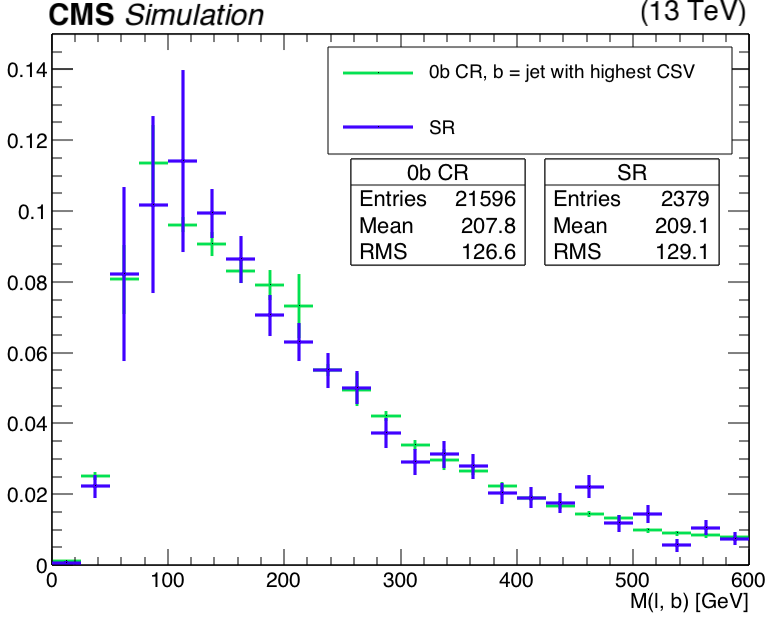
\includegraphics[width=0.4\textwidth]{figures/cr0b_Mlbshape_AB.png}
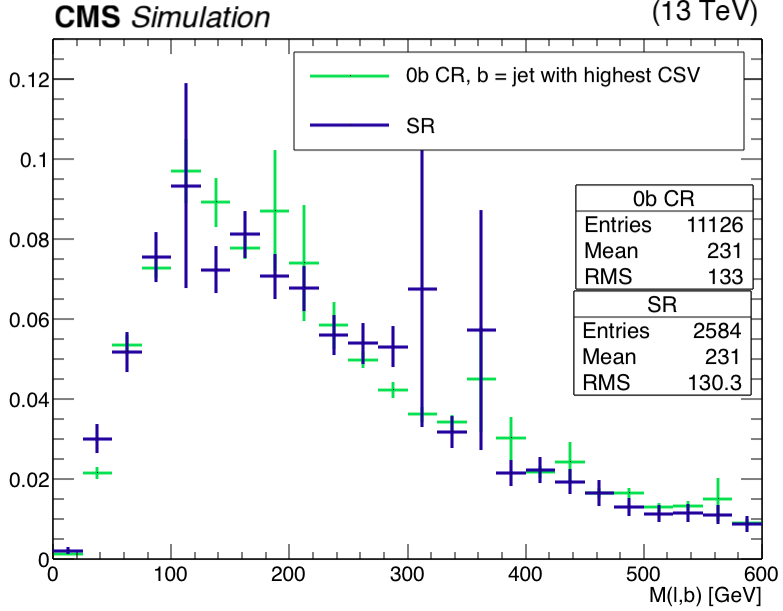
\includegraphics[width=0.4\textwidth]{figures/cr0b_Mlbshape_CD.png}
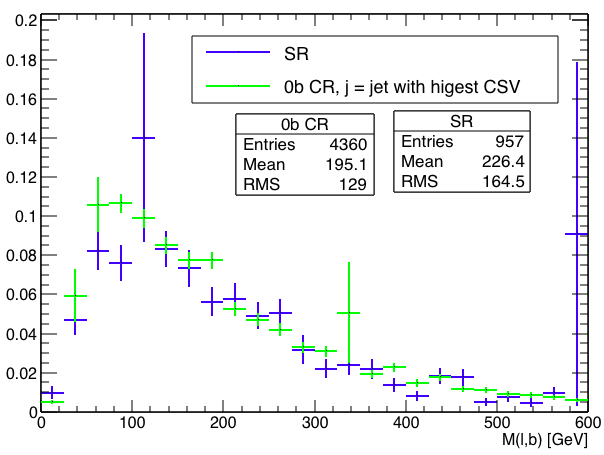
\includegraphics[width=0.4\textwidth]{figures/cr0b_Mlbshape_EF.png}
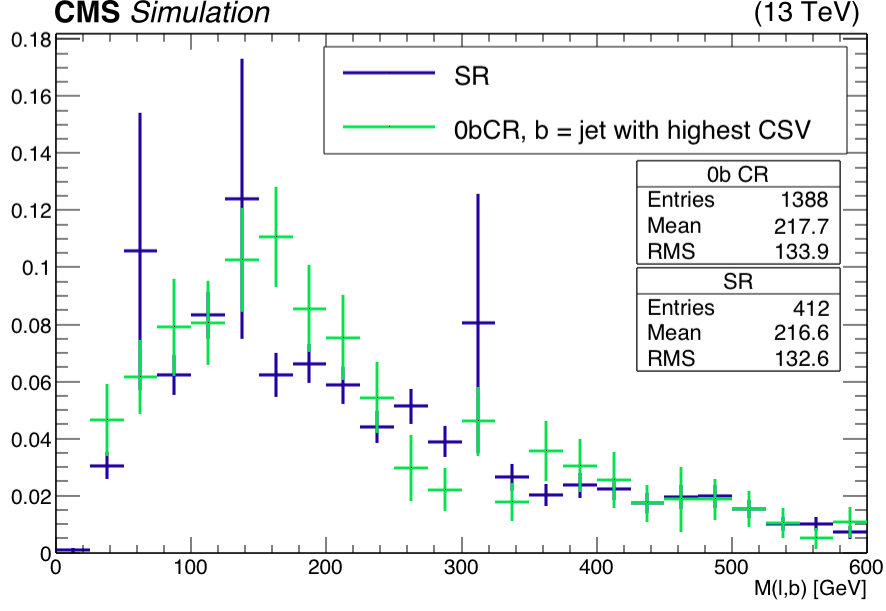
\includegraphics[width=0.4\textwidth]{figures/cr0b_Mlbshape_GH.png}
\caption{Comparison between $M_{\ell b}$ from SRs and makeshift $M_{\ell
    b}$ from CRs, using simulated data. The four plots are made in the
  combined A+B regions, the C+D regions, the E+F regions, and the G+H
  regions, respectively.}
\label{fig:stop:1lw:mlb}
\end{figure}

\begin{figure}[htbp]
\centering
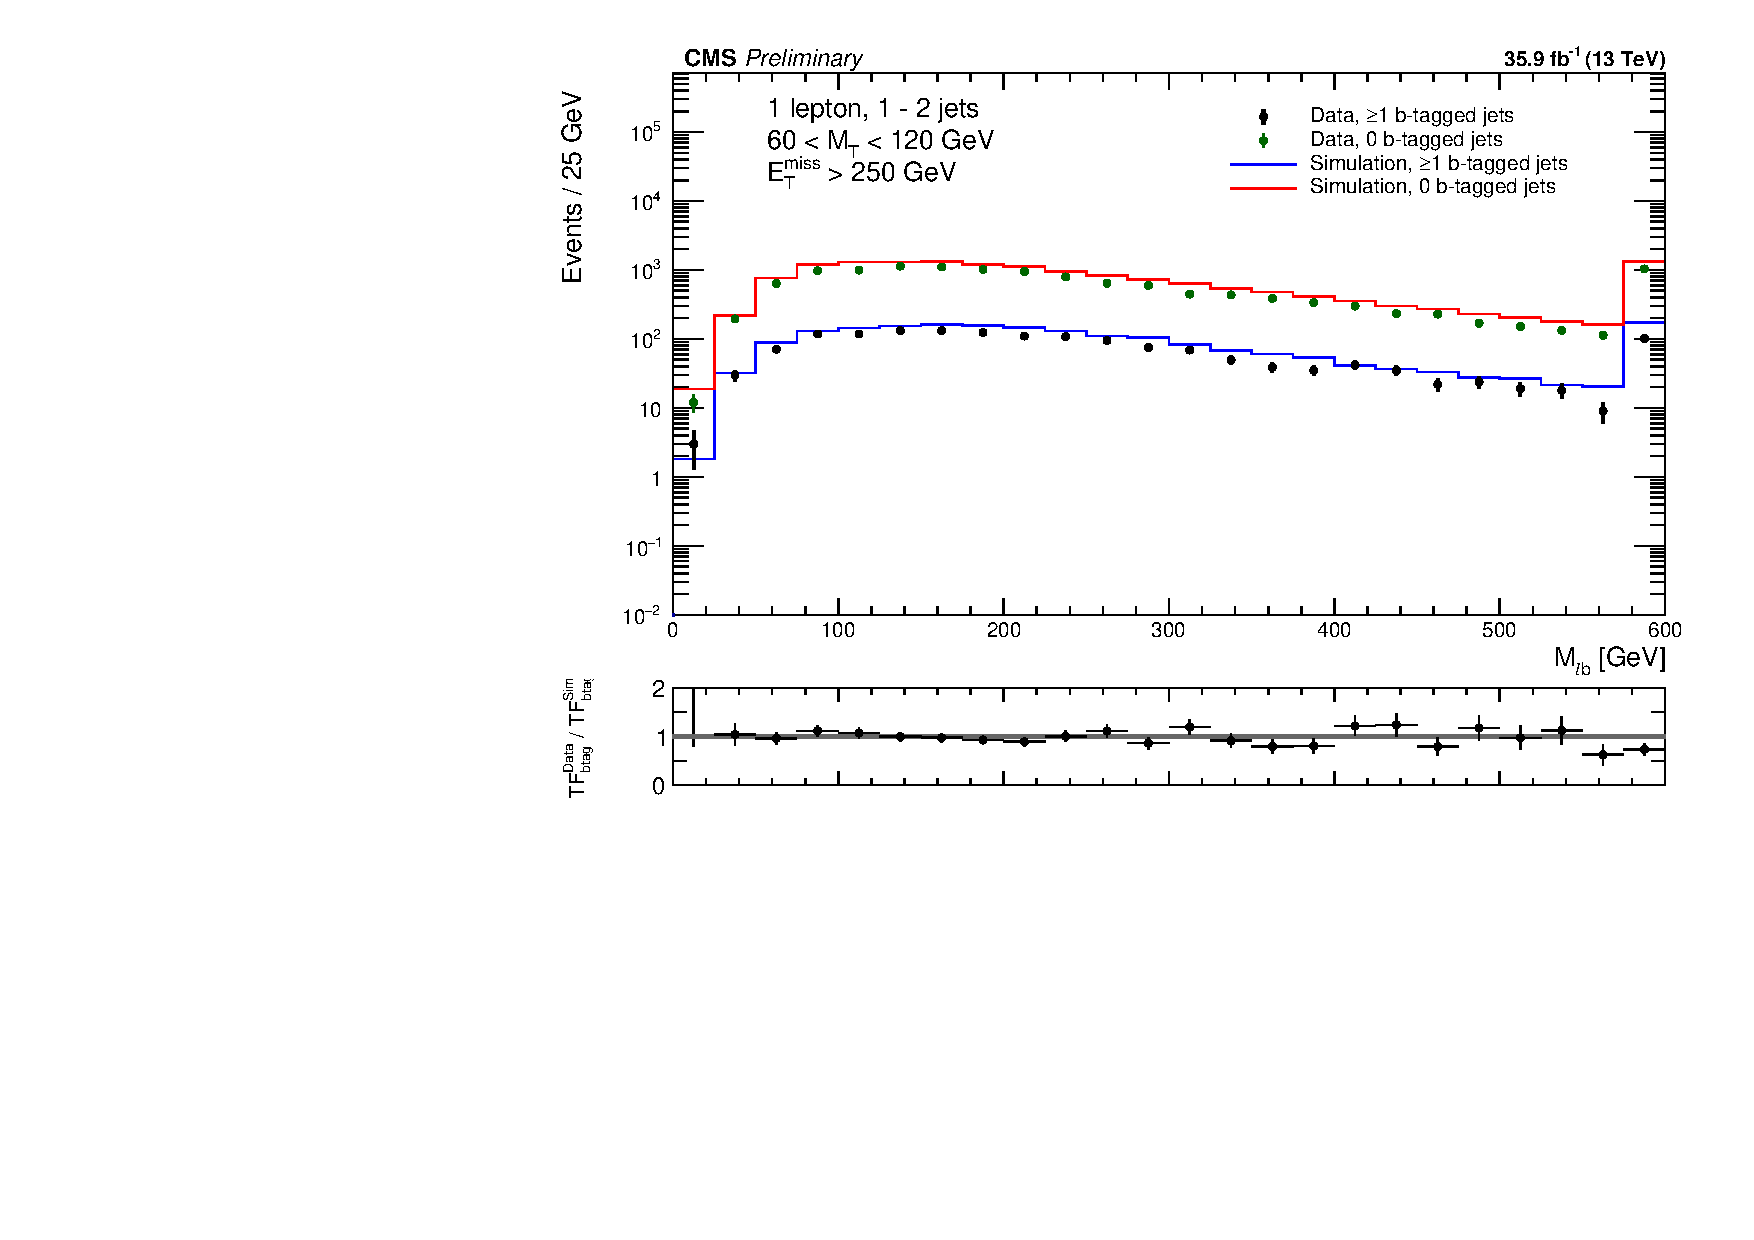
\includegraphics[width=0.8\textwidth]{figures/cr0b_Mlbshape_crosscheck.pdf}
\caption{Comparison of $M_{\ell b}$ shape for data and MC, in 0-btag
  and $\geq$1-btag crosscheck regions.}
\label{fig:stop:1lw:mlbxcheck}
\end{figure}

The yields for data and MC in the control regions are given in Table
\ref{tab:stop:1lw:cryields}. The MC simulations receive all the same
corrections as in the SRs. The purity of these control regions ranges
from a high of 83\% to a low of 37\%. The impurity of these regions
will be addressed further on with a systematic uncertainty.

% Yield table hand-made using the common looper.
% Have NOT checked this against tables in the AN! %%%%%%%%%%%%%%%%%%%%%%%%%%%
\begin{sidewaystable}
\centering
\scriptsize
\caption{Data and Monte Carlo yields in the 0-btag control regions,
  based on 35.9 fb$^{-1}$ of luminosity.}
\label{tab:stop:1lw:cryields}
\begin{tabular}{|l|c c c c c|c|c|}
\hline
Region  & $\ge2$~leptons & $1$~lepton,~from~$W$ & $1$~lepton,~from~$t$ & $Z\rightarrow\nu\nu$ & Sum Bkg. & Data & Data/MC \\*
\hline \hline
% A regions
$<4$jets,~modTopness$\ge10$,~$M_{lb}<175$,~$250<MET<350$  & 30.78 $\pm$ 2.14  & 96.44 $\pm$ 2.92  & 0.47 $\pm$ 0.27  & 14.22 $\pm$ 2.00  & 141.91 $\pm$ 4.15  & 151 $\pm$ 12.29  & 1.06 $\pm$ 0.09 \\*
$<4$jets,~modTopness$\ge10$,~$M_{lb}<175$,~$350<MET<450$  & 10.30 $\pm$ 1.23  & 49.02 $\pm$ 2.21  & 0.33 $\pm$ 0.23  & 9.30 $\pm$ 1.36  & 68.95 $\pm$ 2.89  & 68 $\pm$ 8.25  & 0.99 $\pm$ 0.13 \\*
$<4$jets,~modTopness$\ge10$,~$M_{lb}<175$,~$450<MET<600$  & 3.63 $\pm$ 0.80  & 26.07 $\pm$ 1.77  & ---  & 4.55 $\pm$ 1.05  & 34.25 $\pm$ 2.21  & 31 $\pm$ 5.57  & 0.91 $\pm$ 0.17 \\*
$<4$jets,~modTopness$\ge10$,~$M_{lb}<175$,~$MET>600$  & 0.36 $\pm$ 0.18  & 7.56 $\pm$ 0.41  & ---  & 1.17 $\pm$ 0.52  & 9.09 $\pm$ 0.69  & 11 $\pm$ 3.32  & 1.21 $\pm$ 0.38 \\*
\hline
% B regions
$<4$jets,~modTopness$\ge10$,~$M_{lb}\ge175$,~$250<MET<450$  & 18.27 $\pm$ 1.70  & 163.16 $\pm$ 1.83  & ---  & 21.95 $\pm$ 2.31  & 203.38 $\pm$ 3.40  & 232 $\pm$ 15.23  & 1.14 $\pm$ 0.08 \\*
$<4$jets,~modTopness$\ge10$,~$M_{lb}\ge175$,~$450<MET<650$  & 2.86 $\pm$ 0.73  & 47.58 $\pm$ 1.48  & ---  & 9.50 $\pm$ 1.41  & 59.94 $\pm$ 2.17  & 48 $\pm$ 6.93  & 0.80 $\pm$ 0.12 \\*
$<4$jets,~modTopness$\ge10$,~$M_{lb}\ge175$,~$MET>600$  & 0.57 $\pm$ 0.32  & 29.39 $\pm$ 1.76  & ---  & 4.30 $\pm$ 1.08  & 34.26 $\pm$ 2.09  & 27 $\pm$ 5.20  & 0.79 $\pm$ 0.16 \\*
\hline
% C regions
$\ge4$jets,~modTopness$<0.0$,~$M_{lb}<175$,~$250<MET<350$  & 77.99 $\pm$ 2.93  & 54.11 $\pm$ 2.25  & 4.98 $\pm$ 0.85  & 8.70 $\pm$ 1.16  & 145.79 $\pm$ 3.96  & 143 $\pm$ 11.96  & 0.98 $\pm$ 0.09 \\*
$\ge4$jets,~modTopness$<0.0$,~$M_{lb}<175$,~$350<MET<450$  & 16.61 $\pm$ 1.46  & 17.36 $\pm$ 1.66  & 0.64 $\pm$ 0.29  & 3.69 $\pm$ 0.86  & 38.30 $\pm$ 2.39  & 31 $\pm$ 5.57  & 0.81 $\pm$ 0.15 \\*
$\ge4$jets,~modTopness$<0.0$,~$M_{lb}<175$,~$450<MET<550$  & 4.25 $\pm$ 0.77  & 4.06 $\pm$ 0.29  & 0.29 $\pm$ 0.21  & 1.71 $\pm$ 0.59  & 10.30 $\pm$ 1.04  & 5 $\pm$ 2.24  & 0.49 $\pm$ 0.22 \\*
$\ge4$jets,~modTopness$<0.0$,~$M_{lb}<175$,~$550<MET<650$  & 0.80 $\pm$ 0.28  & 1.70 $\pm$ 0.22  & ---  & 0.09 $\pm$ 0.02  & 2.58 $\pm$ 0.36  & 3 $\pm$ 1.73  & 1.16 $\pm$ 0.69 \\*
$\ge4$jets,~modTopness$<0.0$,~$M_{lb}<175$,~$MET>650$  & 0.94 $\pm$ 0.36  & 1.30 $\pm$ 0.17  & 0.14 $\pm$ 0.14  & 0.32 $\pm$ 0.26  & 2.70 $\pm$ 0.50  & 4 $\pm$ 2.00  & 1.48 $\pm$ 0.79 \\*
\hline
% D regions
$\ge4$jets,~modTopness$<0.0$,~$M_{lb}\ge175$,~$250<MET<350$  & 58.54 $\pm$ 2.66  & 95.51 $\pm$ 5.39  & 5.51 $\pm$ 0.84  & 8.45 $\pm$ 1.32  & 168.01 $\pm$ 6.21  & 137 $\pm$ 11.70  & 0.82 $\pm$ 0.08 \\*
$\ge4$jets,~modTopness$<0.0$,~$M_{lb}\ge175$,~$350<MET<450$  & 17.31 $\pm$ 1.43  & 36.16 $\pm$ 3.89  & 0.79 $\pm$ 0.31  & 6.11 $\pm$ 1.05  & 60.37 $\pm$ 4.29  & 36 $\pm$ 6.00  & 0.60 $\pm$ 0.11 \\*
$\ge4$jets,~modTopness$<0.0$,~$M_{lb}\ge175$,~$450<MET<550$  & 5.24 $\pm$ 0.79  & 12.01 $\pm$ 0.53  & 0.00 $\pm$ 0.00  & 1.58 $\pm$ 0.68  & 18.83 $\pm$ 1.17  & 11 $\pm$ 3.32  & 0.58 $\pm$ 0.18 \\*
$\ge4$jets,~modTopness$<0.0$,~$M_{lb}\ge175$,~$MET>550$  & 4.74 $\pm$ 1.33  & 10.38 $\pm$ 0.50  & 0.39 $\pm$ 0.22  & 1.25 $\pm$ 0.56  & 16.76 $\pm$ 1.55  & 13 $\pm$ 3.61  & 0.78 $\pm$ 0.23 \\*
\hline
% E regions
$\ge4$jets,~$0.0<$modTopness$<10$,~$M_{lb}<175$,~$250<MET<350$  & 16.34 $\pm$ 1.33  & 27.47 $\pm$ 3.52  & 0.28 $\pm$ 0.20  & 4.75 $\pm$ 0.79  & 48.84 $\pm$ 3.85  & 54 $\pm$ 7.35  & 1.11 $\pm$ 0.17 \\*
$\ge4$jets,~$0.0<$modTopness$<10$,~$M_{lb}<175$,~$350<MET<550$  & 4.76 $\pm$ 0.78  & 13.35 $\pm$ 0.53  & 0.13 $\pm$ 0.12  & 1.67 $\pm$ 0.62  & 19.91 $\pm$ 1.13  & 13 $\pm$ 3.61  & 0.65 $\pm$ 0.18 \\*
$\ge4$jets,~$0.0<$modTopness$<10$,~$M_{lb}<175$,~$MET>550$  & 0.27 $\pm$ 0.16  & 1.48 $\pm$ 0.17  & ---  & 0.74 $\pm$ 0.40  & 2.49 $\pm$ 0.46  & 2 $\pm$ 1.41  & 0.80 $\pm$ 0.59 \\*
\hline
% F regions
$\ge4$jets,~$0.0<$modTopness$<10$,~$M_{lb}\ge175$,~$250<MET<450$  & 6.34 $\pm$ 0.80  & 33.10 $\pm$ 1.48  & 0.05 $\pm$ 0.05  & 4.91 $\pm$ 0.94  & 44.40 $\pm$ 1.93  & 50 $\pm$ 7.07  & 1.13 $\pm$ 0.17 \\*
$\ge4$jets,~$0.0<$modTopness$<10$,~$M_{lb}\ge175$,~$MET>450$  & 1.30 $\pm$ 0.59  & 8.71 $\pm$ 0.41  & ---  & 2.46 $\pm$ 0.61  & 12.47 $\pm$ 0.95  & 5 $\pm$ 2.24  & 0.40 $\pm$ 0.18 \\*
\hline
% G regions
$\ge4$jets,~modTopness$\ge10$,~$M_{lb}<175$,~$250<MET<350$  & 1.57 $\pm$ 0.37  & 1.74 $\pm$ 0.18  & 0.15 $\pm$ 0.15  & 0.57 $\pm$ 0.24  & 4.03 $\pm$ 0.49  & 7 $\pm$ 2.65  & 1.74 $\pm$ 0.69 \\*
$\ge4$jets,~modTopness$\ge10$,~$M_{lb}<175$,~$350<MET<450$  & 1.69 $\pm$ 0.42  & 3.94 $\pm$ 1.10  & ---  & 0.25 $\pm$ 0.03  & 5.88 $\pm$ 1.18  & 7 $\pm$ 2.65  & 1.19 $\pm$ 0.51 \\*
$\ge4$jets,~modTopness$\ge10$,~$M_{lb}<175$,~$450<MET<600$  & 1.28 $\pm$ 0.50  & 3.08 $\pm$ 0.25  & ---  & 0.50 $\pm$ 0.43  & 4.86 $\pm$ 0.70  & 3 $\pm$ 1.73  & 0.62 $\pm$ 0.37 \\*
$\ge4$jets,~modTopness$\ge10$,~$M_{lb}<175$,~$MET>600$  & 0.64 $\pm$ 0.37  & 2.58 $\pm$ 1.13  & ---  & 0.31 $\pm$ 0.44  & 3.53 $\pm$ 1.27  & 2 $\pm$ 1.41  & 0.57 $\pm$ 0.45 \\*
\hline
% H regions
$\ge4$jets,~modTopness$\ge10$,~$M_{lb}\ge175$,~$250<MET<450$  & 3.15 $\pm$ 0.90  & 6.65 $\pm$ 0.36  & 0.11 $\pm$ 0.11  & 0.93 $\pm$ 0.28  & 10.84 $\pm$ 1.02  & 12 $\pm$ 3.46  & 1.11 $\pm$ 0.34 \\*
$\ge4$jets,~modTopness$\ge10$,~$M_{lb}\ge175$,~$MET>450$  & 1.82 $\pm$ 0.54  & 9.65 $\pm$ 0.44  & ---  & 2.68 $\pm$ 0.59  & 14.15 $\pm$ 0.91  & 9 $\pm$ 3.00  & 0.64 $\pm$ 0.22 \\*
\hline
% I regions
Compressed search, $250<MET<350$  & 19.70 $\pm$ 1.43  & 23.62 $\pm$ 4.24  & 1.80 $\pm$ 0.45  & 2.36 $\pm$ 0.52  & 47.47 $\pm$ 4.53  & 49 $\pm$ 7.00  & 1.03 $\pm$ 0.18 \\*
Compressed search, $350<MET<450$  & 7.49 $\pm$ 0.92  & 12.07 $\pm$ 3.64  & 0.40 $\pm$ 0.21  & 2.43 $\pm$ 0.76  & 22.38 $\pm$ 3.83  & 11 $\pm$ 3.32  & 0.49 $\pm$ 0.17 \\*
Compressed search, $450<MET<550$  & 2.98 $\pm$ 0.67  & 3.68 $\pm$ 0.27  & 0.30 $\pm$ 0.22  & 1.75 $\pm$ 0.53  & 8.71 $\pm$ 0.92  & 5 $\pm$ 2.24  & 0.57 $\pm$ 0.26 \\*
Compressed search, $MET>550$  & 1.43 $\pm$ 0.43  & 3.26 $\pm$ 0.26  & ---  & 1.13 $\pm$ 0.48  & 5.82 $\pm$ 0.70  & 3 $\pm$ 1.73  & 0.52 $\pm$ 0.30 \\*
\hline
\end{tabular}
\end{sidewaystable}

\subsubsection{Systematic Uncertainties}
\label{sssec:stop:1lw:systematics}

Many of the systematic uncertainties on the 1$\ell$W background are
assessed the same way as for the lost lepton background, as described
in Section \ref{sssec:stop:lostlep:systematics}. These uncertainties
are:
\begin{itemize}
\item Data and MC statistics
\item b-tagging efficiencies
\item JES
\item PDF
\item $Q^2$
\item $\met$ resolution
\end{itemize}
% Note: Table from common looper includes several other systematics
% not mentioned in the AN.

Because our $TF_\text{btag}$ is derived from simulation, we must ensure that
the relative cross-sections of W+b and W+non-b jets are correctly
modeled in MC. We check the agreement between data and MC on number of
b-jets in the high-statistics crosscheck region described above. As
Figure \ref{fig:stop:1lw:wb} shows, a 50\% systematic uncertainty on
the W+b cross section adequately covers any mismodeling that may
exist. Additionally, the 0-btag CRs have considerable impurity from
non-1$\ell$W backgrounds, so we assess a 50\% systematic uncertainty on
that contamination. The systematic uncertainties on the single lepton
from W estimate are presented in Table \ref{tab:stop:1lw:systematics}.

% Plot of W+b crosscheck, taken from AN-16-463. Unpublished.
\begin{figure}[htb]
\centering
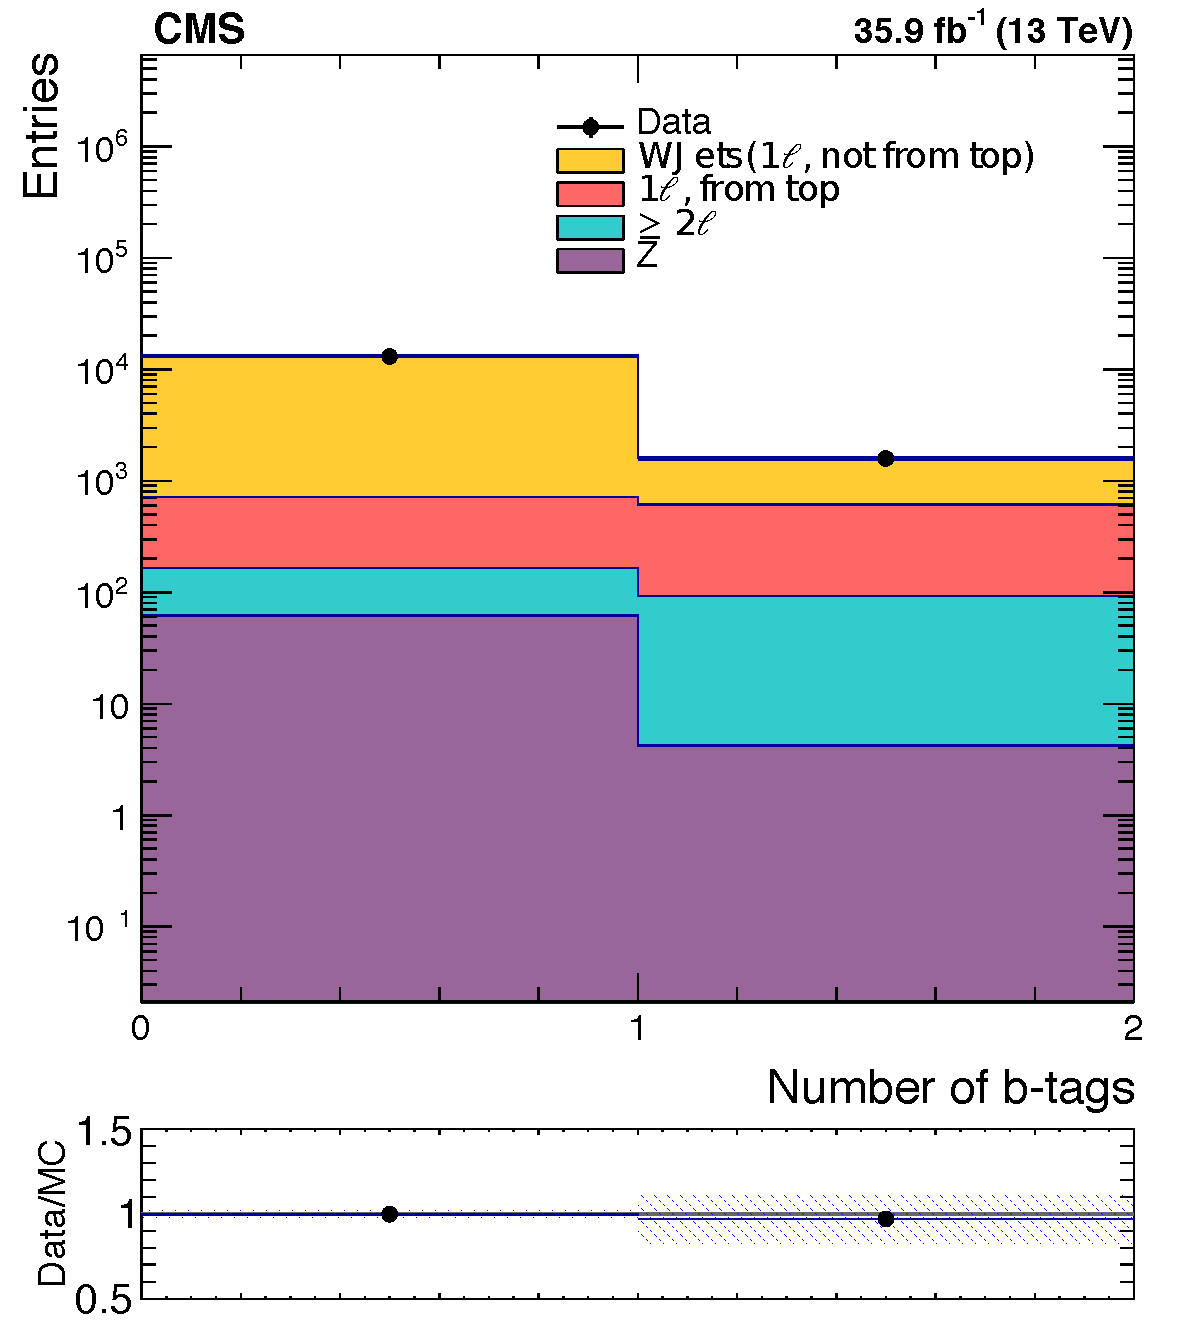
\includegraphics[width=0.45\textwidth]{Figures/cr0b_nbtags_crosscheck.pdf}
\caption{Number of b-tags compared between data and MC, in
  high-statistics crosscheck region. The second bin includes events
  with one or more b-tags. The uncertainty band illustrates a 50\%
  uncertainty on the W+b cross section}
\label{fig:stop:1lw:wb}
\end{figure}

% Systematics table goes here. Should probably check it against the AN...
% ALSO, need to add in the corridor systematics too!
\begin{table}[htb]
\centering
\tiny
\caption{Summary of systematic uncertainties on single lepton from W
  background estimate.}
\label{tab:stop:1lw:systematics}
\scalebox{0.4}{
\begin{tabular}{|l|c|c|c|c|c|c|c|c|c|c|c|c|c|c|c|c|c|c|c|c|c|c|c|c|c|c|c|} \hline
Systematic  & A  & A  & A  & A  & B  & B  & B  & C  & C  & C  & C  & C  & D  & D  & D  & D  & E  & E  & E  & F  & F  & G  & G  & G  & G  & H  & H \\
 & $250-350$  & $350-450$  & $450-600$  & $>600$  & $250-450$  & $450-600$  & $>600$  & $250-350$  & $350-450$  & $450-550$  & $550-650$  & $>650$  & $250-350$  & $350-450$  & $450-550$  & $>550$  & $250-350$  & $350-550$  & $>550$  & $250-450$  & $>450$  & $250-350$  & $350-450$  & $450-600$  & $>600$  & $250-450$  & $>450$ \\ \hline \hline
Data Stats & 8.1\%  & 12.1\%  & 18.0\%  & 30.2\%  & 6.6\%  & 14.4\%  & 19.2\%  & 8.4\%  & 18.0\%  & 44.7\%  & 57.7\%  & 50.0\%  & 8.5\%  & 16.7\%  & 30.2\%  & 27.7\%  & 13.6\%  & 27.7\%  & 70.7\%  & 14.1\%  & 44.7\%  & 37.8\%  & 37.8\%  & 57.7\%  & 70.7\%  & 28.9\%  & 33.3\% \\
MC Stats & 5.8\%  & 7.7\%  & 11.5\%  & 20.8\%  & 6.7\%  & 10.9\%  & 14.2\%  & 12.2\%  & 12.2\%  & 20.1\%  & 31.0\%  & 33.3\%  & 7.3\%  & 12.5\%  & 19.0\%  & 22.5\%  & 22.7\%  & 11.4\%  & 30.1\%  & 9.8\%  & 19.2\%  & 21.9\%  & 20.8\%  & 21.2\%  & 27.0\%  & 18.8\%  & 19.2\% \\ \hline
CR Impurity & 19.1\%  & 16.9\%  & 13.6\%  & 9.2\%  & 11.0\%  & 11.5\%  & 7.7\%  & 45.9\%  & 37.6\%  & 43.5\%  & 20.6\%  & 35.0\%  & 27.5\%  & 25.1\%  & 22.1\%  & 23.5\%  & 28.0\%  & 19.7\%  & 25.5\%  & 14.6\%  & 17.8\%  & 39.7\%  & 19.7\%  & 22.4\%  & 15.6\%  & 24.0\%  & 18.9\% \\
JES  & 3.6\%  & 4.8\%  & 6.7\%  & 5.6\%  & 1.0\%  & 5.2\%  & 0.1\%  & 13.7\%  & 10.4\%  & 16.3\%  & 7.9\%  & 4.7\%  & 1.1\%  & 3.9\%  & 11.5\%  & 1.1\%  & 2.2\%  & 9.3\%  & 0.9\%  & 7.8\%  & 7.2\%  & 11.3\%  & 36.1\%  & 3.9\%  & 4.7\%  & 18.7\%  & 1.8\% \\
ISR  & 0.2\%  & 0.2\%  & 0.1\%  & 0.2\%  & 0.2\%  & 0.1\%  & 0.0\%  & 7.7\%  & 6.2\%  & 4.9\%  & 3.8\%  & 3.9\%  & 5.2\%  & 4.3\%  & 3.4\%  & 1.3\%  & 4.9\%  & 3.6\%  & 3.1\%  & 2.1\%  & 0.3\%  & 7.3\%  & 4.1\%  & 1.6\%  & 0.5\%  & 3.7\%  & 0.4\% \\
MET~Resolution  & 0.1\%  & 0.4\%  & 1.3\%  & 0.9\%  & 0.0\%  & 0.8\%  & 1.5\%  & 0.0\%  & 0.5\%  & 0.8\%  & 0.2\%  & 0.0\%  & 0.0\%  & 0.4\%  & 0.1\%  & 1.3\%  & 0.0\%  & 0.4\%  & 1.3\%  & 0.1\%  & 0.4\%  & 0.1\%  & 0.6\%  & 0.8\%  & 1.9\%  & 0.0\%  & 0.8\% \\
bTag~Efficicency,~Heavy~Flavour  & 2.1\%  & 1.8\%  & 1.6\%  & 1.2\%  & 2.3\%  & 2.5\%  & 4.2\%  & 3.4\%  & 2.7\%  & 1.9\%  & 3.0\%  & 2.5\%  & 3.1\%  & 2.8\%  & 2.8\%  & 2.2\%  & 3.2\%  & 2.6\%  & 1.5\%  & 2.5\%  & 2.6\%  & 2.7\%  & 2.5\%  & 2.2\%  & 1.9\%  & 2.7\%  & 2.8\% \\
bTag~Efficicency,~Light~Flavour  & 2.8\%  & 3.4\%  & 3.2\%  & 5.5\%  & 2.8\%  & 2.0\%  & 1.7\%  & 2.9\%  & 3.5\%  & 2.8\%  & 4.9\%  & 2.4\%  & 1.8\%  & 1.7\%  & 1.6\%  & 1.8\%  & 2.6\%  & 3.5\%  & 4.3\%  & 1.3\%  & 2.2\%  & 2.3\%  & 2.6\%  & 4.8\%  & 3.5\%  & 0.9\%  & 2.0\% \\
Lepton~Scale~Factor  & 0.4\%  & 0.3\%  & 0.8\%  & 0.2\%  & 0.2\%  & 0.4\%  & 0.2\%  & 1.1\%  & 2.4\%  & 0.8\%  & 0.3\%  & 0.2\%  & 1.0\%  & 1.5\%  & 1.3\%  & 1.7\%  & 0.3\%  & 0.5\%  & 0.2\%  & 0.3\%  & 0.2\%  & 0.3\%  & 1.0\%  & 5.7\%  & 0.1\%  & 0.7\%  & 1.3\% \\
$\tau$~Efficiency~SF  & 0.1\%  & 0.0\%  & 0.0\%  & 0.0\%  & 0.0\%  & 0.0\%  & 0.0\%  & 0.3\%  & 0.2\%  & 0.3\%  & 0.2\%  & 0.3\%  & 0.2\%  & 0.2\%  & 0.2\%  & 0.2\%  & 0.1\%  & 0.2\%  & 0.1\%  & 0.1\%  & 0.1\%  & 0.3\%  & 0.1\%  & 0.1\%  & 0.0\%  & 0.1\%  & 0.1\% \\
${\nu}p_{T}$  & 2.3\%  & 3.1\%  & 1.8\%  & 0.6\%  & 2.3\%  & 0.5\%  & 0.2\%  & 1.1\%  & 4.8\%  & 2.7\%  & 2.7\%  & 6.0\%  & 5.4\%  & 6.3\%  & 6.9\%  & 6.1\%  & 4.4\%  & 4.6\%  & 2.1\%  & 3.0\%  & 3.8\%  & 6.4\%  & 6.9\%  & 8.2\%  & 5.6\%  & 5.7\%  & 4.2\% \\
$W$~Width  & 0.7\%  & 0.5\%  & 0.4\%  & 0.2\%  & 0.3\%  & 0.2\%  & 0.1\%  & 0.3\%  & 0.8\%  & 0.4\%  & 0.3\%  & 0.8\%  & 1.2\%  & 0.9\%  & 0.8\%  & 0.7\%  & 1.0\%  & 0.6\%  & 0.2\%  & 0.6\%  & 0.4\%  & 1.4\%  & 1.0\%  & 1.0\%  & 0.6\%  & 1.0\%  & 0.5\% \\
$W+HF$~x-section  & 23.0\%  & 21.2\%  & 25.3\%  & 15.5\%  & 35.8\%  & 32.9\%  & 35.8\%  & 2.9\%  & 6.9\%  & 7.2\%  & 3.4\%  & 10.3\%  & 21.6\%  & 21.0\%  & 28.5\%  & 14.5\%  & 10.8\%  & 15.9\%  & 24.5\%  & 33.2\%  & 34.2\%  & 24.0\%  & 24.3\%  & 22.4\%  & 25.7\%  & 36.6\%  & 30.9\% \\
Pileup~Reweight  & 1.1\%  & 1.8\%  & 0.7\%  & 3.2\%  & 1.3\%  & 1.5\%  & 1.6\%  & 1.6\%  & 1.3\%  & 1.1\%  & 3.4\%  & 8.8\%  & 0.8\%  & 2.5\%  & 3.4\%  & 0.7\%  & 3.9\%  & 0.9\%  & 6.0\%  & 2.9\%  & 3.4\%  & 4.6\%  & 6.8\%  & 3.9\%  & 4.5\%  & 1.2\%  & 0.2\% \\
PDF  & 7.5\%  & 9.1\%  & 9.0\%  & 7.8\%  & 8.5\%  & 9.4\%  & 8.3\%  & 1.7\%  & 7.7\%  & 9.1\%  & 2.9\%  & 13.1\%  & 1.6\%  & 8.1\%  & 3.0\%  & 7.8\%  & 7.2\%  & 4.8\%  & 18.4\%  & 4.3\%  & 8.9\%  & 6.7\%  & 1.9\%  & 10.1\%  & 3.2\%  & 2.4\%  & 13.7\% \\
$\alpha_{S}$  & 0.7\%  & 1.3\%  & 0.4\%  & 4.0\%  & 6.0\%  & 2.5\%  & 2.3\%  & 1.8\%  & 2.6\%  & 1.8\%  & 1.4\%  & 1.5\%  & 0.9\%  & 1.1\%  & 1.8\%  & 1.2\%  & 1.2\%  & 1.5\%  & 1.5\%  & 4.5\%  & 2.7\%  & 1.7\%  & 2.0\%  & 0.7\%  & 0.8\%  & 6.4\%  & 1.2\% \\
$Q^{2}$  & 2.9\%  & 4.0\%  & 2.2\%  & 1.0\%  & 1.9\%  & 3.1\%  & 2.6\%  & 3.3\%  & 4.3\%  & 5.1\%  & 2.6\%  & 7.6\%  & 2.0\%  & 3.7\%  & 0.7\%  & 2.8\%  & 5.2\%  & 2.7\%  & 1.7\%  & 1.5\%  & 1.9\%  & 7.8\%  & 3.4\%  & 3.4\%  & 1.1\%  & 3.8\%  & 2.0\% \\
\hline
Total  & 27.0\%  & 28.4\%  & 35.3\%  & 41.6\%  & 38.8\%  & 39.4\%  & 44.3\%  & 22.7\%  & 28.3\%  & 53.7\%  & 66.7\%  & 64.1\%  & 25.9\%  & 32.4\%  & 48.0\%  & 40.1\%  & 31.3\%  & 36.4\%  & 83.2\%  & 39.1\%  & 61.0\%  & 53.4\%  & 62.5\%  & 67.5\%  & 80.6\%  & 54.7\%  & 51.6\% \\ \hline
\end{tabular}}
\end{table}

\subsubsection{Results}
\label{sssec:stop:1lw:results}

The full results of the single lepton from W background estimate,
including systematic uncertainties, are presented in Table
\ref{tab:stop:1lw:results}.

% 1lW estimate results, made using the common looper.
% Have NOT checked these against the results in the AN! %%%%%%%%%%%%%%%
\begin{sidewaystable}
\centering
\small
\caption{Summary of the single lepton from W background estimate, and
  all its key components.}
\label{tab:stop:1lw:results}
\begin{tabular}{|l|c|c|c|c|c|} \hline
Region & MET bin & Observed$_\text{CR}$ & Purity & $TF_\text{btag}$ & SR Estimate \\ \hline \hline
 $<4$jets,~tmod$\ge10.0$,~$mlb<175$ & $250<MET<350$  & 151 $\pm$ 12.29  & 0.68 $\pm$ 0.14  & 0.07 $\pm$ 0.02  & 7.15 $\pm$ 1.93  \\
 $<4$jets,~tmod$\ge10.0$,~$mlb<175$ & $350<MET<450$  & 68 $\pm$ 8.25  & 0.71 $\pm$ 0.15  & 0.08 $\pm$ 0.02  & 4.08 $\pm$ 1.16  \\
 $<4$jets,~tmod$\ge10.0$,~$mlb<175$ & $450<MET<600$  & 31 $\pm$ 5.57  & 0.76 $\pm$ 0.13  & 0.07 $\pm$ 0.02  & 1.75 $\pm$ 0.62  \\
 $<4$jets,~tmod$\ge10.0$,~$mlb<175$ & $MET>600$      & 11 $\pm$ 3.32  & 0.83 $\pm$ 0.13  & 0.09 $\pm$ 0.02  & 0.80 $\pm$ 0.33  \\
\hline
 $<4$jets,~tmod$\ge10.0$,~$mlb\ge175$ & $250<MET<450$  & 232 $\pm$ 15.23  & 0.80 $\pm$ 0.11  & 0.03 $\pm$ 0.01  & 5.60 $\pm$ 2.17  \\
 $<4$jets,~tmod$\ge10.0$,~$mlb\ge175$ & $450<MET<600$  & 48 $\pm$ 6.93  & 0.79 $\pm$ 0.13  & 0.04 $\pm$ 0.01  & 1.56 $\pm$ 0.62  \\
 $<4$jets,~tmod$\ge10.0$,~$mlb\ge175$ & $MET>600$      & 27 $\pm$ 5.20  & 0.86 $\pm$ 0.11  & 0.04 $\pm$ 0.01  & 0.89 $\pm$ 0.40  \\
\hline
 $\ge4$jets,~tmod$<0.0$,~$mlb<175$ & $250<MET<350$  & 143 $\pm$ 11.96  & 0.37 $\pm$ 0.18  & 0.18 $\pm$ 0.04  & 9.79 $\pm$ 2.22  \\
 $\ge4$jets,~tmod$<0.0$,~$mlb<175$ & $350<MET<450$  & 31 $\pm$ 5.57  & 0.45 $\pm$ 0.18  & 0.17 $\pm$ 0.03  & 2.35 $\pm$ 0.67  \\
 $\ge4$jets,~tmod$<0.0$,~$mlb<175$ & $450<MET<550$  & 5 $\pm$ 2.24  & 0.39 $\pm$ 0.20  & 0.23 $\pm$ 0.08  & 0.45 $\pm$ 0.24  \\
 $\ge4$jets,~tmod$<0.0$,~$mlb<175$ & $550<MET<650$  & 3 $\pm$ 1.73  & 0.66 $\pm$ 0.16  & 0.14 $\pm$ 0.04  & 0.28 $\pm$ 0.19  \\
 $\ge4$jets,~tmod$<0.0$,~$mlb<175$ & $MET>650$      & 4 $\pm$ 2.00  & 0.48 $\pm$ 0.20  & 0.23 $\pm$ 0.09  & 0.45 $\pm$ 0.29  \\
\hline
 $\ge4$jets,~tmod$<0.0$,~$mlb\ge175$ & $250<MET<350$  & 137 $\pm$ 11.70  & 0.57 $\pm$ 0.16  & 0.09 $\pm$ 0.02  & 6.80 $\pm$ 1.76  \\
 $\ge4$jets,~tmod$<0.0$,~$mlb\ge175$ & $350<MET<450$  & 36 $\pm$ 6.00  & 0.60 $\pm$ 0.17  & 0.09 $\pm$ 0.02  & 1.90 $\pm$ 0.62  \\
 $\ge4$jets,~tmod$<0.0$,~$mlb\ge175$ & $450<MET<550$  & 11 $\pm$ 3.32  & 0.64 $\pm$ 0.16  & 0.08 $\pm$ 0.03  & 0.55 $\pm$ 0.26  \\
 $\ge4$jets,~tmod$<0.0$,~$mlb\ge175$ & $MET>550$      & 13 $\pm$ 3.61  & 0.62 $\pm$ 0.17  & 0.14 $\pm$ 0.04  & 1.13 $\pm$ 0.45  \\
\hline
 $\ge4$jets,~$0.0<$tmod$<10.0$,~$mlb<175$ & $250<MET<350$  & 54 $\pm$ 7.35  & 0.56 $\pm$ 0.17  & 0.19 $\pm$ 0.05  & 5.66 $\pm$ 1.77  \\
 $\ge4$jets,~$0.0<$tmod$<10.0$,~$mlb<175$ & $350<MET<550$  & 13 $\pm$ 3.61  & 0.67 $\pm$ 0.15  & 0.14 $\pm$ 0.03  & 1.23 $\pm$ 0.45  \\
 $\ge4$jets,~$0.0<$tmod$<10.0$,~$mlb<175$ & $MET>550$      & 2 $\pm$ 1.41  & 0.59 $\pm$ 0.22  & 0.23 $\pm$ 0.08  & 0.28 $\pm$ 0.23  \\
\hline
 $\ge4$jets,~$0.0<$tmod$<10.0$,~$mlb\ge175$ & $250<MET<450$  & 50 $\pm$ 7.07  & 0.75 $\pm$ 0.13  & 0.08 $\pm$ 0.03  & 2.95 $\pm$ 1.15  \\
 $\ge4$jets,~$0.0<$tmod$<10.0$,~$mlb\ge175$ & $MET>450$      & 5 $\pm$ 2.24  & 0.70 $\pm$ 0.17  & 0.07 $\pm$ 0.03  & 0.26 $\pm$ 0.16  \\
\hline
 $\ge4$jets,~tmod$\ge10.0$,~$mlb<175$ & $250<MET<350$  & 7 $\pm$ 2.65  & 0.43 $\pm$ 0.19  & 0.33 $\pm$ 0.10  & 1.00 $\pm$ 0.53  \\
 $\ge4$jets,~tmod$\ge10.0$,~$mlb<175$ & $350<MET<450$  & 7 $\pm$ 2.65  & 0.67 $\pm$ 0.22  & 0.16 $\pm$ 0.12  & 0.76 $\pm$ 0.48  \\
 $\ge4$jets,~tmod$\ge10.0$,~$mlb<175$ & $450<MET<600$  & 3 $\pm$ 1.73  & 0.63 $\pm$ 0.19  & 0.24 $\pm$ 0.07  & 0.45 $\pm$ 0.31  \\
 $\ge4$jets,~tmod$\ge10.0$,~$mlb<175$ & $MET>600$      & 2 $\pm$ 1.41  & 0.73 $\pm$ 0.21  & 0.25 $\pm$ 0.08  & 0.36 $\pm$ 0.29  \\
\hline
 $\ge4$jets,~tmod$\ge10.0$,~$mlb\ge175$ & $250<MET<450$  & 12 $\pm$ 3.46  & 0.61 $\pm$ 0.17  & 0.14 $\pm$ 0.06  & 1.01 $\pm$ 0.55  \\
 $\ge4$jets,~tmod$\ge10.0$,~$mlb\ge175$ & $MET>450$      & 9 $\pm$ 3.00  & 0.68 $\pm$ 0.16  & 0.09 $\pm$ 0.03  & 0.55 $\pm$ 0.28  \\
\hline
Compressed search & $250<MET<350$  & 49 $\pm$ 7.00  & 0.50 $\pm$ 0.19  & 0.21 $\pm$ 0.06  & 5.03 $\pm$ 1.78  \\
Compressed search & $350<MET<450$  & 11 $\pm$ 3.32  & 0.54 $\pm$ 0.20  & 0.14 $\pm$ 0.03  & 0.84 $\pm$ 0.33  \\
Compressed search & $450<MET<550$  & 5 $\pm$ 2.24   & 0.42 $\pm$ 0.19  & 0.20 $\pm$ 0.05  & 0.42 $\pm$ 0.24  \\
Compressed search & $MET>550$      & 3 $\pm$ 1.73  & 0.56 $\pm$ 0.19  & 0.14 $\pm$ 0.05  & 0.24 $\pm$ 0.17  \\
\hline
\end{tabular}
\end{sidewaystable}

\subsection{Single Lepton from Top}
\label{ssec:stop:1ltop}

At the start of our search, before making any cuts to the data, the
main background to contend with was genuine single leptons that result
from top quarks decaying to W-bosons, which in turn decay
leptonically. However, as earlier sections have mentioned, our high
$\met$ and $\mt$ requirements are extremely effective at reducing this
background component. So much so, in fact, that after event
selections, the single lepton from top background (or 1$\ell$top) becomes
practically negligible in all our signal regions.

Unfortunately, there is no way to perform a robust, data-driven
estimate of this background, because we cannot construct a control
region that is enhanced in 1$\ell$top processes (mostly $\ttonelep$,
followed by single top quark production). Since this background was so
strongly reduced by the $\mt$ cut, one might consider a lower-$\mt$
sideband region; however, as we discovered in the previous section,
such a region contains a considerable number of 1$\ell$W events, and
even lost lepton events. Therefore, we are forced to estimate the
1$\ell$top background directly from Monte Carlo simulation.

As mentioned in Section \ref{sec:stop:searchstrategy}, most 1$\ell$top
events that pass the $\mt$ cut do so because of $\met$ resolution
effects. Therefore, by far the most dominant uncertainty on the 1$\ell
t$ background component is the uncertainty on $\met$ resolution. Our
studies in [APPENDIX] show this uncertainty can be as high as 25\%. In
Figure \ref{fig:stop:1ltop:metres}, we show the $\met$ spectra of
$\ttonelep$ events from Monte Carlo, both before and after fluctuating
the $\met$ resolution according to the uncertainties from
[APPENDIX]. We note that the yields in the various bins may fluctuate
by 100\% or more as the $\met$ resolution is fluctuated. On that
basis, we assign a flat 100\% uncertainty to the 1$\ell$top background
component. All other uncertainties, including statistical, are
insignificant by comparison, and should be covered by the 100\%
uncertainty we impose.

% MET resolution fluctuation plots, from AN-16-463. Unpublished.
\begin{figure}
\centering
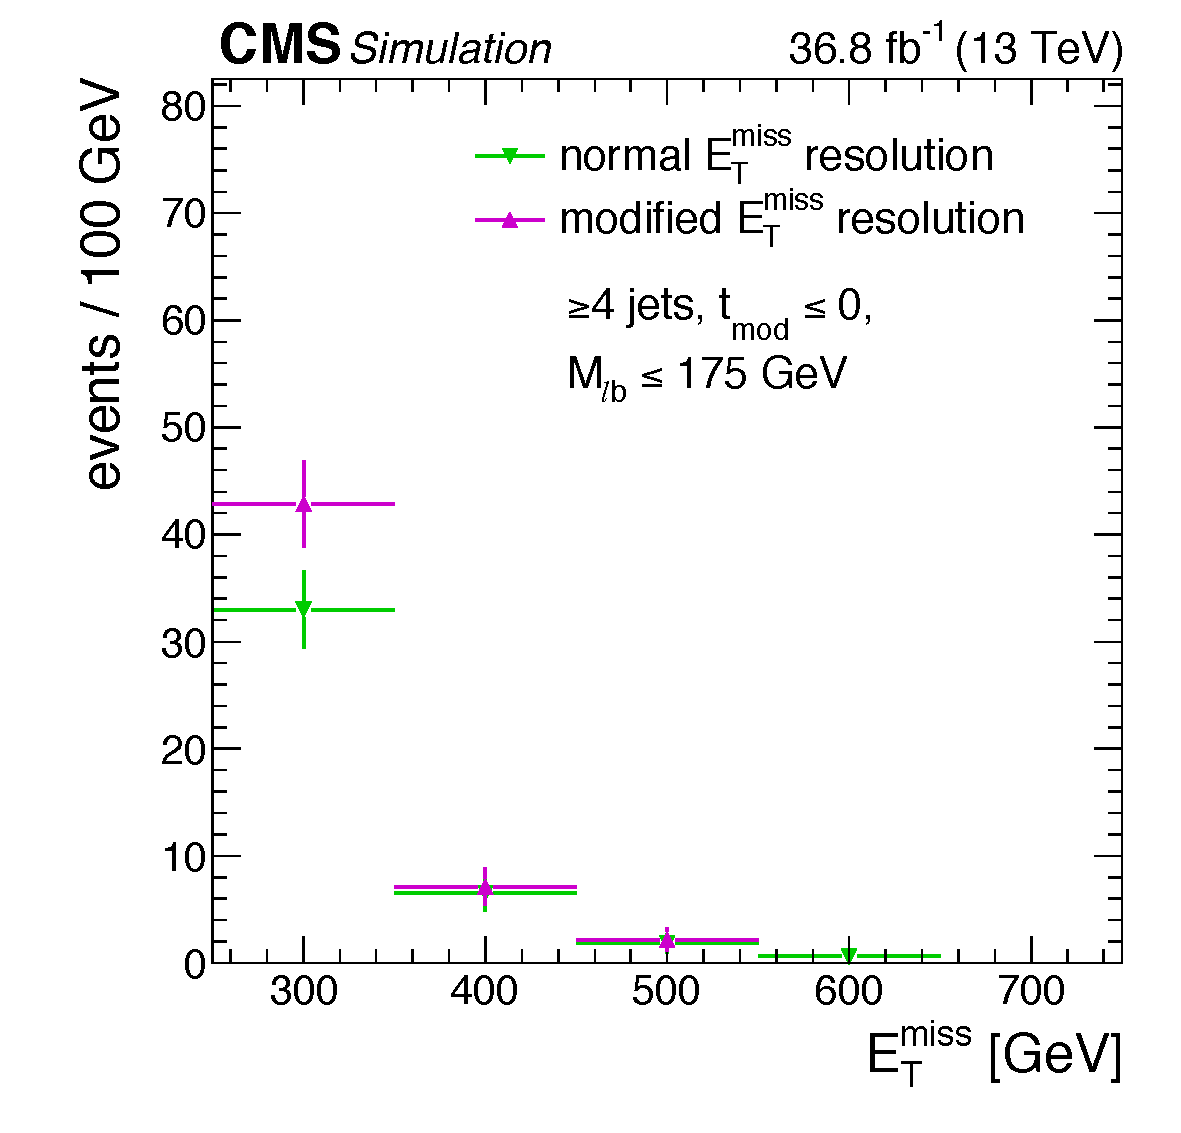
\includegraphics[width=0.45\textwidth]{figures/metres_1ltop_C.pdf}
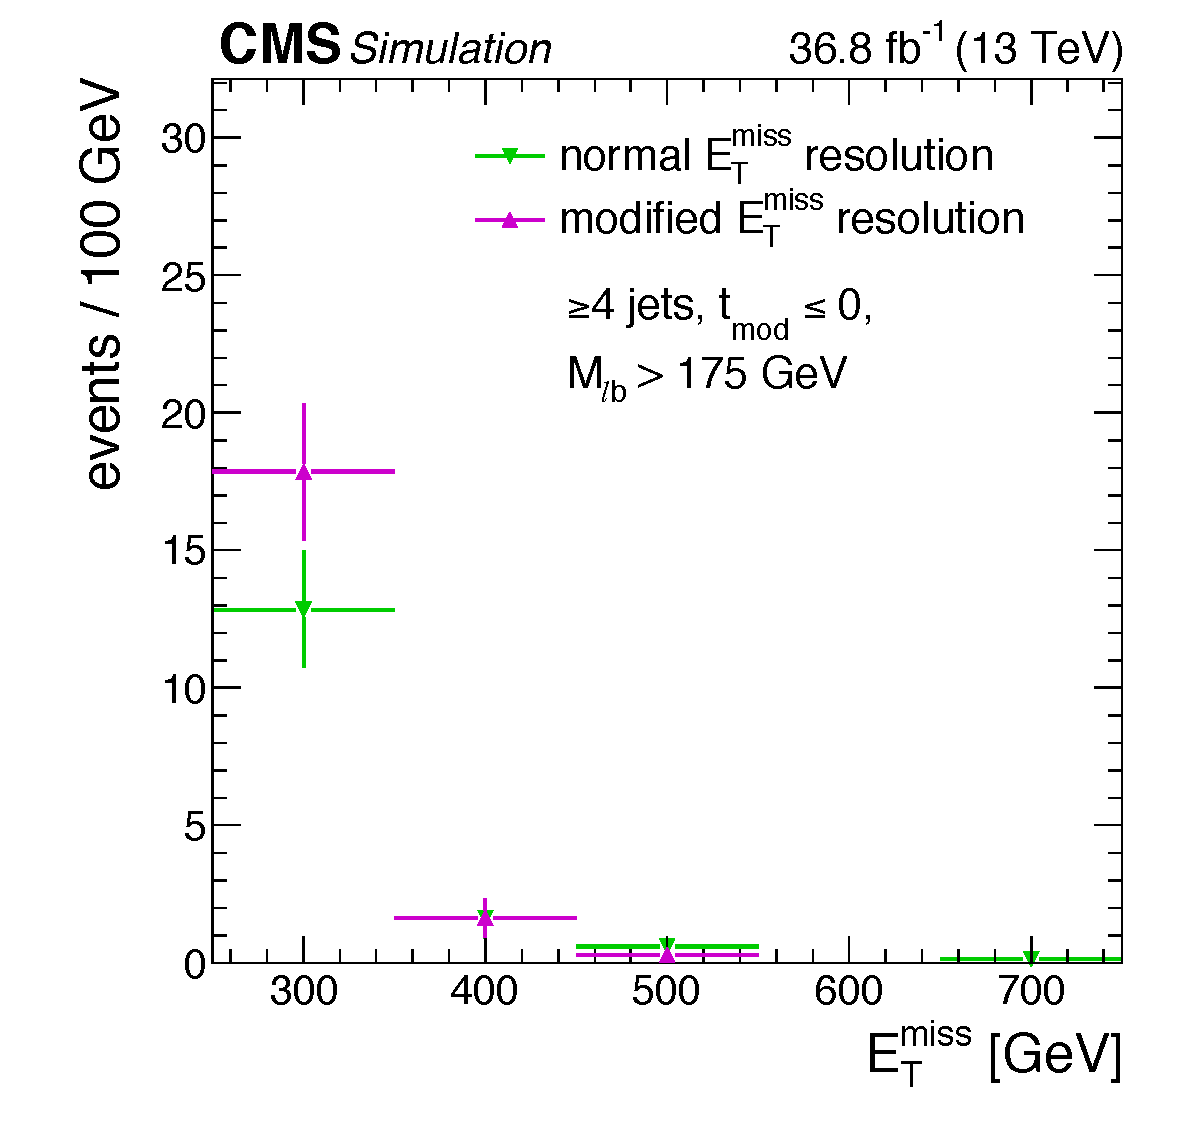
\includegraphics[width=0.45\textwidth]{figures/metres_1ltop_D.pdf}
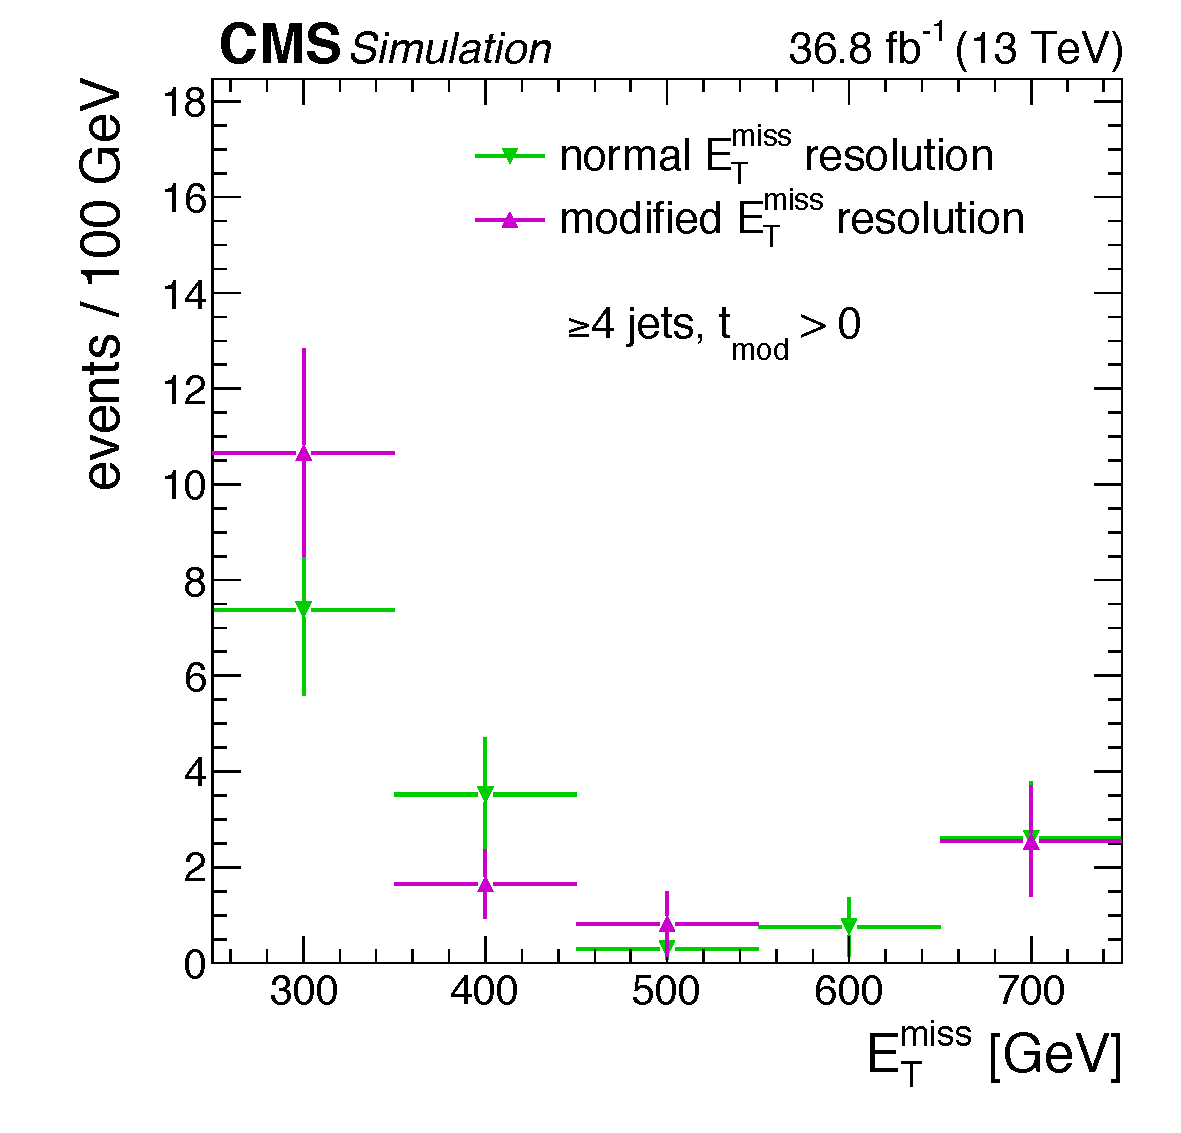
\includegraphics[width=0.45\textwidth]{figures/metres_1ltop_EFGH.pdf}
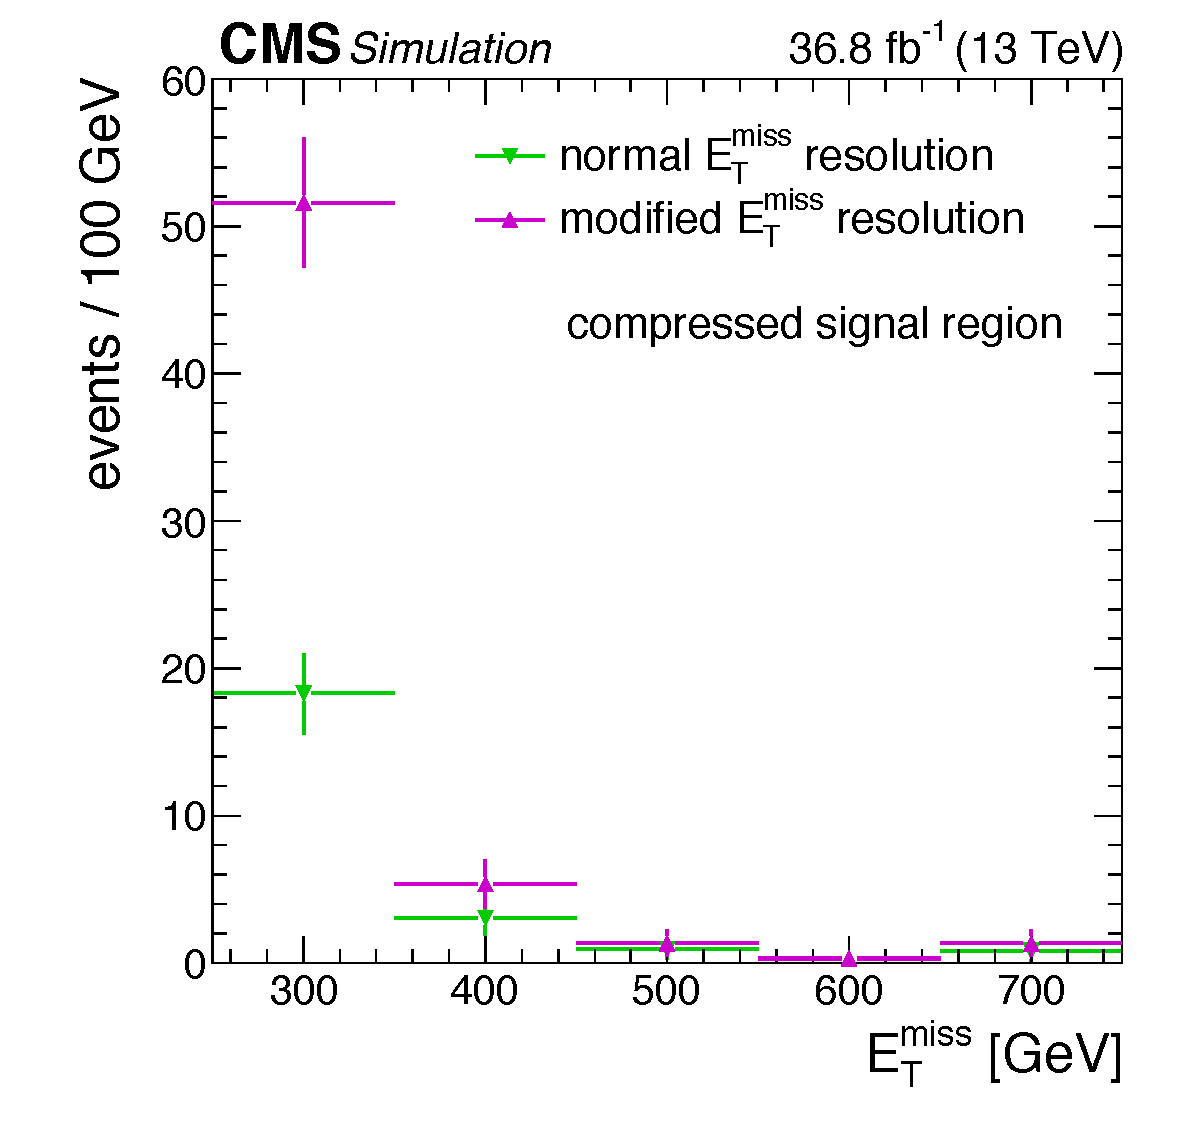
\includegraphics[width=0.45\textwidth]{figures/metres_1ltop_I.pdf}
\caption{$\met$ distributions in $\ttonelep$ Monte Carlo, with and
  without fluctuated $\met$ resolution. The plots are made
  in the C regions, the D regions, the combined E/F/G/H regions, and
  the I (corridor) regions, respectively. The A/B regions have an
  insignificant $\ttonelep$ component, so are not shown.}
\label{fig:stop:1ltop:metres}
\end{figure}

The final results of our single lepton from top background estimate
are presented in Table \ref{tab:stop:1ltop:results}.

% 1ltop background table. Numbers come from paper draft. Everything
% else I cobbled together from bits and pieces of other stuff.
\begin{table}[htbp]
\centering
\caption{Results of the single lepton from top background estimate,
  with 100\% uncertainty applied.}
\label{tab:stop:1ltop:results}
\begin{tabular}{|l|c|c|}
\hline
Region & MET bin & SR Estimate\\
\hline
$<4$jets,~tmod$\ge10.0$,~$mlb<175$ & $250<MET<350$ &  ---  \\
$<4$jets,~tmod$\ge10.0$,~$mlb<175$ & $350<MET<450$ &  0.22$\pm$0.22 \\
$<4$jets,~tmod$\ge10.0$,~$mlb<175$ & $450<MET<600$ &  0.13$\pm$0.13  \\
$<4$jets,~tmod$\ge10.0$,~$mlb<175$ & $MET>600$     &  0.28$\pm$0.28 \\
\hline
$<4$jets,~tmod$\ge10.0$,~$mlb\ge175$ & $250<MET<450$ &  --- \\
$<4$jets,~tmod$\ge10.0$,~$mlb\ge175$ & $450<MET<600$ &  ---  \\
$<4$jets,~tmod$\ge10.0$,~$mlb\ge175$ & $MET>600$     &  ---  \\
\hline
$\ge4$jets,~tmod$<0.0$,~$mlb<175$ & $250<MET<350$ &  13.2$\pm$13.2  \\
$\ge4$jets,~tmod$<0.0$,~$mlb<175$ & $350<MET<450$ &  2.3$\pm$2.3  \\
$\ge4$jets,~tmod$<0.0$,~$mlb<175$ & $450<MET<550$ &  0.63$\pm$0.63  \\
$\ge4$jets,~tmod$<0.0$,~$mlb<175$ & $550<MET<650$ &  0.09$\pm$0.09 \\
$\ge4$jets,~tmod$<0.0$,~$mlb<175$ & $MET>650$     &  --- \\
\hline
$\ge4$jets,~tmod$<0.0$,~$mlb\ge175$ & $250<MET<350$ &  3.1$\pm$3.1  \\
$\ge4$jets,~tmod$<0.0$,~$mlb\ge175$ & $350<MET<450$ &  0.59$\pm$0.59  \\
$\ge4$jets,~tmod$<0.0$,~$mlb\ge175$ & $450<MET<550$ &  0.37$\pm$0.37  \\
$\ge4$jets,~tmod$<0.0$,~$mlb\ge175$ & $MET>550$     &  ---  \\
\hline
$\ge4$jets,~$0.0<$tmod$<10.0$,~$mlb<175$ & $250<MET<350$ &  1.7$\pm$1.7  \\
$\ge4$jets,~$0.0<$tmod$<10.0$,~$mlb<175$ & $350<MET<550$ &  0.48$\pm$0.48  \\
$\ge4$jets,~$0.0<$tmod$<10.0$,~$mlb<175$ & $MET>550$     &  0.33$\pm$0.33  \\
\hline
$\ge4$jets,~$0.0<$tmod$<10.0$,~$mlb\ge175$ & $250<MET<450$ &  0.30$\pm$0.30  \\
$\ge4$jets,~$0.0<$tmod$<10.0$,~$mlb\ge175$ & $MET>450$     &  ---  \\
\hline
$\ge4$jets,~tmod$\ge10.0$,~$mlb<175$ & $250<MET<350$ &  0.75$\pm$0.75  \\
$\ge4$jets,~tmod$\ge10.0$,~$mlb<175$ & $350<MET<450$ &  0.69$\pm$0.69  \\
$\ge4$jets,~tmod$\ge10.0$,~$mlb<175$ & $450<MET<600$ &  0.10$\pm$0.10 \\
$\ge4$jets,~tmod$\ge10.0$,~$mlb<175$ & $MET>600$     &  0.65$\pm$0.65  \\
\hline
$\ge4$jets,~tmod$\ge10.0$,~$mlb\ge175$ & $250<MET<450$ &  ---  \\
$\ge4$jets,~tmod$\ge10.0$,~$mlb\ge175$ & $MET>450$     &  0.11$\pm$0.11 \\
\hline
Compressed search & $250<MET<350$ & 5.3$\pm$5.3 \\
Compressed search & $350<MET<450$ & 1.0$\pm$1.0 \\
Compressed search & $450<MET<550$ & 0.12$\pm$0.12 \\
Compressed search & $MET>550$     & 0.13$\pm$0.13 \\
\hline
\end{tabular}
\end{table}

\subsection{Rare Standard Model Processes}
\label{ssec:stop:rarebkg}

The final component to our backgrounds is that from
rare Standard Model processes. In practice, we define this background
component to contain any events containing a Z-boson that decays to
two neutrinos (effectively becoming invisible). The vast majority of
these events come from ttZ production where the Z decays to
neutrinos, especially in the $\geq$4-jet regions. The next largest
source is WZ production, which manifests primarily in the 2-to-3-jet
regions.

\subsubsection{Estimation Method}
\label{sssec:stop:rarebkg:estimation}

Although the rare background is a relatively small component, we still
attempt to estimate it using robust, data-driven methods. In contrast
to the methods used for the lost lepton and 1$\ell$W backgrounds, we
estimate the rare background using a technique more akin to that used
in the top asymmetry measurements, as described in Section
\ref{sec:afb:background}.

Our rare background estimate relies on the assumption that the relative
normalization between data and MC is the same in our signal regions as
in a three-lepton control region. So:
\begin{equation}
\label{eq:stop:rarebkg:rationm}
\frac{N_\text{rare}^\text{SR}}{M_\text{rare}^\text{SR}} =
\frac{N_\text{ttZ, WZ}^{CR3\ell}}{M_\text{ttZ, WZ}^{CR3\ell}}
\end{equation}
If we invert Equation \ref{eq:stop:rarebkg:rationm}, we can estimate
our rare background component using the Monte Carlo yield in our
signal region, times a normalization factor derived in the 3$\ell$
control region:
\begin{equation}
\label{eq:stop:rarebkg:estimation}
N_\text{rare}^\text{SR} = M_\text{rare}^\text{SR} \times
NF_\text{ttZ, WZ}^{CR 3\ell}
\end{equation}
The normalization factors are derived using a template fit, separately
for ttZ and WZ production, as shown in Figure
\ref{fig:stop:rarebkg:normalization}. For ttZ, the factor is $1.14 \pm
0.30$, and for WZ, it is $1.26 \pm 0.09$. The uncertainties
incorporate both statistical and systematic factors that influence the
template fit.

% Plots of ttZ and WZ normalization fits, taken from AN-16-386. Unpublished!!
\begin{figure}[htb]
\centering
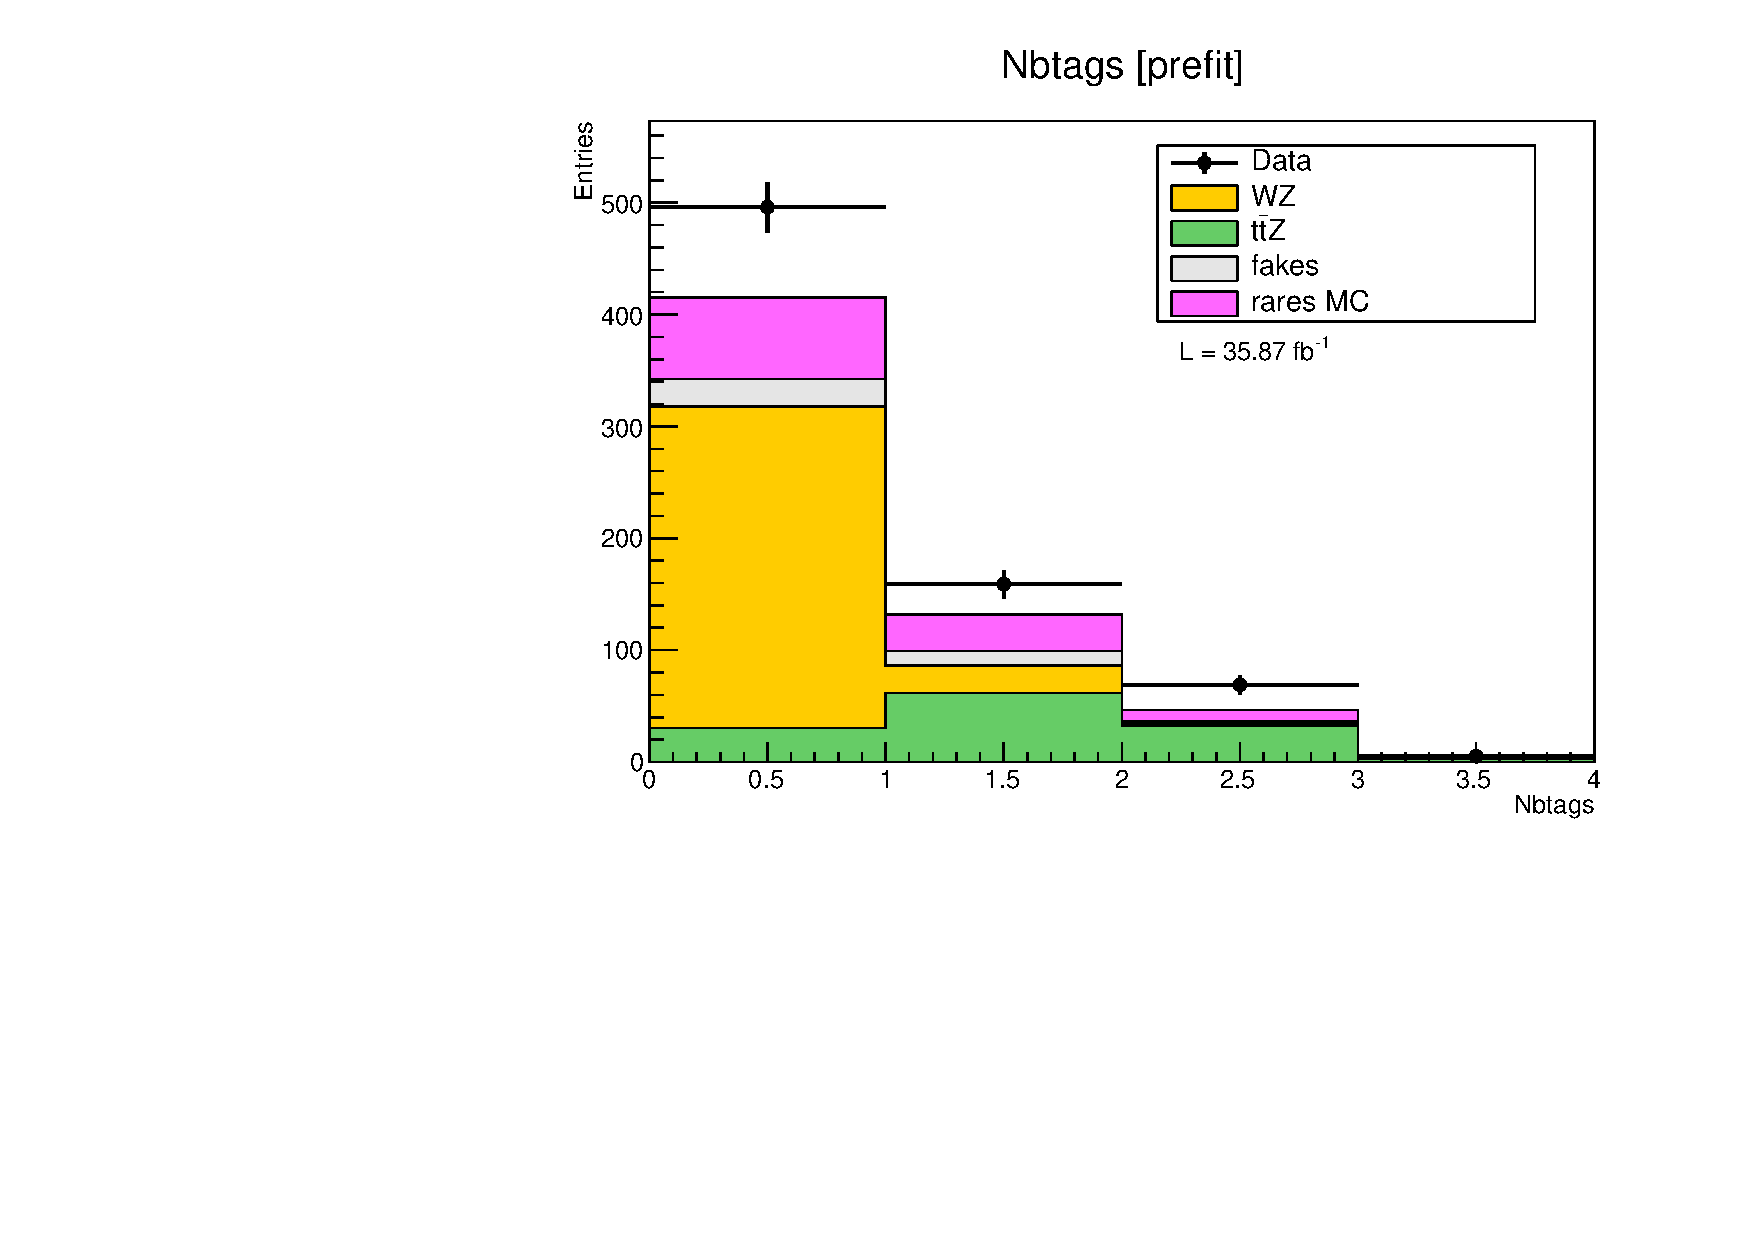
\includegraphics[width=0.45\textwidth]{figures/rarebkg_norm_prefit.pdf}
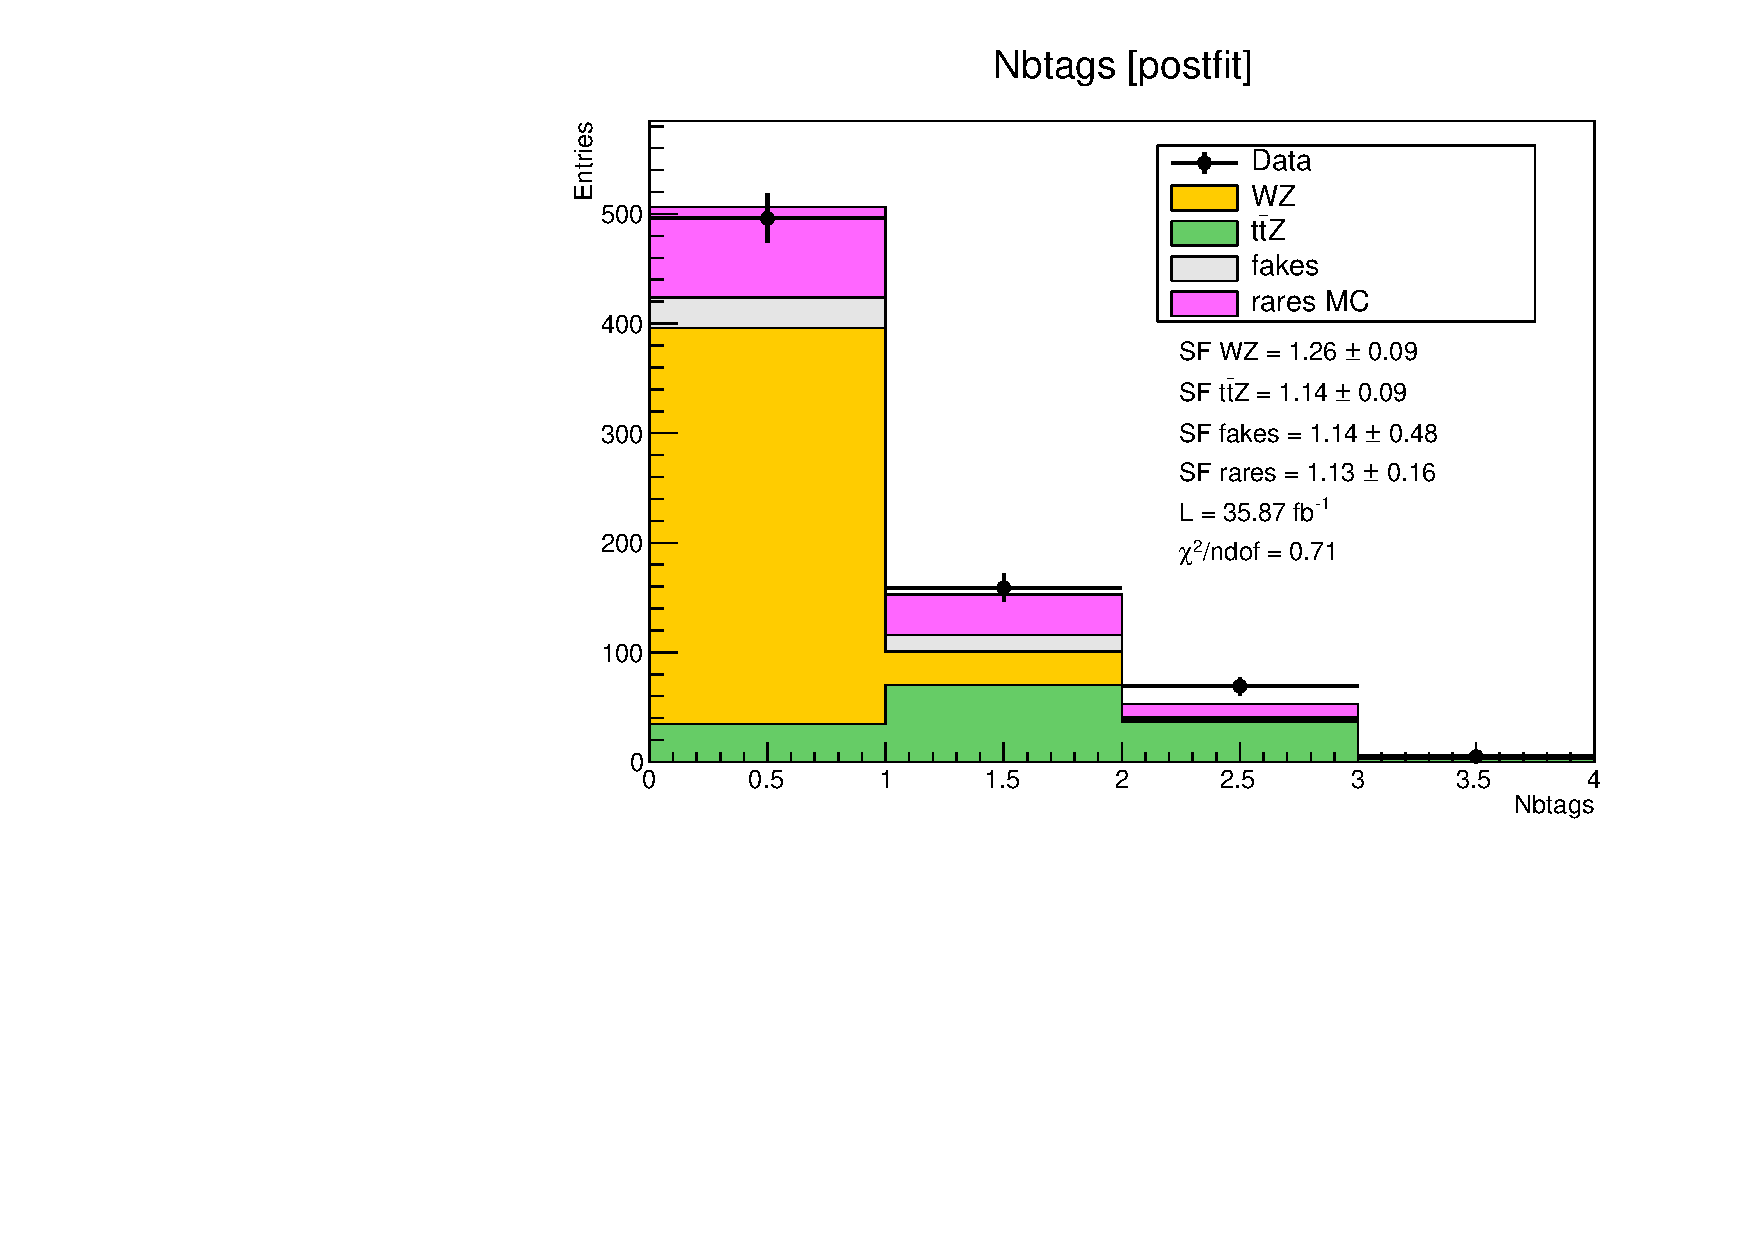
\includegraphics[width=0.45\textwidth]{figures/rarebkg_norm_postfit.pdf}
\caption{Distribution of number of b-jets in 3$\ell$ control region,
  before and after template fit, from 2016 same-sign dilepton search.}
\label{fig:stop:rarebkg:normalization}
\end{figure}

We do not derive these factors ourselves; rather, they are taken
from a CMS internal note documenting changes and improvements to the
2016 same-sign dilepton search. The same-sign analysis was described
in public documentation supporting ICHEP 2016\cite{samesign}.
% AN-2016-386, follow up to PAS SUS-16-020

\subsubsection{Control Region Definition}
\label{sssec:stop:rarebkg:crdefinitions}

The control region used to select 3-lepton events for the same-sign
analysis is formed from the following criteria:
\begin{itemize}
\item Require three leptons ($e$ or $\mu$) passing tight ID
  criteria. The first two must have $p_T >$ 25 and 20 GeV,
  respectively, and the third must have $p_T >$ 10 GeV.
\item The third lepton must form an opposite-sign same-flavor pair
  with one of the first two leptons.
\item The invariant mass of the paired leptons must be within 15 GeV
  of the Z-boson mass (91.1876 GeV \cite{pdg}).
\item There must be at least two jets in the event.
\item The scalar sum of the $p_T$ of the jets, known as $H_T$, must
  be $>$ 80 GeV.
\item $\met >$ 30 GeV
\end{itemize}

\subsubsection{Systematic Uncertainties}
\label{sssec:stop:rarebkg:systematics}

Because the rare background is estimated differently from the other
backgrounds, we assess our systematic uncertainties in two different
ways. The standard experimental systematics are evaluated exactly as
they were for the lost lepton and 1$\ell$W backgrounds, except where
explicitly stated otherwise. The experimental uncertainties include:
\begin{itemize}
\item Monte Carlo statistics
\item b-tagging efficiencies (HF and LF)
\item Lepton ID and isolation efficiencies
\item JES
\item ISR $n_\text{jets}$ reweighting
\item \textbf{Pileup reweighting:} this systematic is highly sensitive to the
  low MC statistics of this background. To avoid large fluctuations,
  we evaluate the uncertainty across all signal regions summed
  together, and see that a conservative 3\% systematic will cover all
  realistic cases.
\end{itemize}

When evaluating the theory uncertainties, we only consider the effects
they have on the shape of the background. We keep the normalization
fixed to the values derived from the control region. And because the
theory uncertainties are highly sensitive to our limited statistics,
we merge several of the nominal regions together by removing the
binning in $M_{\ell b}$ and $t_\text{mod}$. In effect, this leaves us
with fewer regions, binned only in $N_\text{jets}$ and $\met$. The
corridor regions are not merged in any way. This merging is justified
by studies showing that variations in the shapes of $M_{\ell b}$ and
$t_\text{mod}$ are small compared to uncertainties arising from the
$\met$ distribution. The theory uncertainties evaluated in this manner
are:
\begin{itemize}
\item $Q^2$
\item PDF
\item $\alpha_S$
\end{itemize}

The values of the systematic uncertainties are presented in Table
\ref{tab:stop:rarebkg:systematics}

% Table of systematics adapted from AN-16-463.
% May wish to change the layout.
\begin{sidewaystable}
\centering
\footnotesize
\caption{Summary of systematic uncertainties on the rare standard
  model processes background estimate.}
\label{tab:stop:rarebkg:systematics}
\begin{tabular}{|l|cccccccccccc|}
\hline
Region & MC stat.   &   Lep. ID/Iso   &   b-tag (LF) &   b-tag (HF)  &   PU &   PDF &   $\alpha_S$ &   $Q^2$ &   ISR njets  & JES &   Norm.  & Total \\
\hline
 A 250$<\met<$350 & 11.88\% & 0.31\%  & 1.58\%  & 1.23\%  & 3.00\%  & 0.23\%  & 0.86\%  & 3.86\%  & 7.12\%  & 2.55\%  & 20.70\% & 25.60\% \\
 A 350$<\met<$450 & 25.04\% & 0.35\%  & 3.63\%  & 0.77\%  & 3.00\%  & 3.33\%  & 0.61\%  & 1.31\%  & 9.09\%  & 0.37\%  & 24.38\% & 36.61\% \\
 A 450$<\met<$600 & 23.87\% & 0.37\%  & 1.34\%  & 1.34\%  & 3.00\%  & 0.45\%  & 0.39\%  & 2.47\%  & 7.02\%  & 0.46\%  & 20.77\% & 32.71\% \\
 A $\met>$600     & 51.43\% & 0.41\%  & 2.87\%  & 1.74\%  & 3.00\%  & 8.04\%  & 0.36\%  & 2.37\%  & 5.13\%  & 10.54\% & 16.77\% & 56.17\% \\
 B 250$<\met<$450 & 29.98\% & 0.50\%  & 1.67\%  & 1.23\%  & 3.00\%  & 1.17\%  & 0.76\%  & 2.86\%  & 3.97\%  & 1.01\%  & 14.74\% & 34.01\% \\
 B 450$<\met<$600 & 86.04\% & 0.77\%  & 5.28\%  & 1.26\%  & 3.00\%  & 0.45\%  & 0.40\%  & 2.47\%  & 4.00\%  & 32.62\% & 15.46\% & 93.63\% \\
 B $\met>$600     & 228.31\%& 2.65\%  & 19.40\% & 1.64\%  & 3.00\%  & 8.03\%  & 0.36\%  & 2.37\%  & 8.12\%  & 44.04\% & 22.72\% & 234.76\%\\
 C 250$<\met<$350 & 4.56\%  & 0.45\%  & 0.06\%  & 0.68\%  & 3.00\%  & 0.81\%  & 0.60\%  & 1.77\%  & 0.40\%  & 4.78\%  & 26.18\% & 27.26\% \\
 C 350$<\met<$450 & 10.85\% & 0.35\%  & 0.48\%  & 0.66\%  & 3.00\%  & 2.01\%  & 1.23\%  & 5.00\%  & 0.99\%  & 6.85\%  & 23.73\% & 27.73\% \\
 C 450$<\met<$550 & 20.70\% & 0.31\%  & 4.53\%  & 0.26\%  & 3.00\%  & 1.89\%  & 1.34\%  & 4.86\%  & 2.03\%  & 4.52\%  & 18.54\% & 29.25\% \\
 C 550$<\met<$650 & 9.20\%  & 0.38\%  & 0.77\%  & 0.38\%  & 3.00\%  & 4.90\%  & 1.86\%  & 3.67\%  & 3.67\%  & 2.14\%  & 26.32\% & 29.09\% \\
 C $\met>$650     & 12.73\% & 0.45\%  & 0.20\%  & 0.40\%  & 3.00\%  & 8.11\%  & 3.08\%  & 4.23\%  & 4.92\%  & 5.74\%  & 26.32\% & 31.85\% \\
 D 250$<\met<$350 & 19.82\% & 0.31\%  & 0.72\%  & 0.41\%  & 3.00\%  & 0.81\%  & 0.60\%  & 1.76\%  & 0.82\%  & 9.76\%  & 20.24\% & 30.20\% \\
 D 350$<\met<$450 & 27.58\% & 0.32\%  & 1.82\%  & 1.08\%  & 3.00\%  & 2.02\%  & 1.23\%  & 4.99\%  & 1.63\%  & 10.79\% & 17.33\% & 34.98\% \\
 D 450$<\met<$550 & 47.40\% & 0.33\%  & 4.96\%  & 0.22\%  & 3.00\%  & 1.88\%  & 1.33\%  & 4.85\%  & 2.24\%  & 17.87\% & 17.31\% & 54.17\% \\
 D $\met>$550     & 18.94\% & 0.44\%  & 0.06\%  & 0.83\%  & 3.00\%  & 7.53\%  & 2.44\%  & 2.55\%  & 7.31\%  & 7.15\%  & 26.32\% & 35.14\% \\
 E 250$<\met<$350 & 5.55\%  & 0.42\%  & 0.65\%  & 0.74\%  & 3.00\%  & 0.81\%  & 0.60\%  & 1.77\%  & 2.52\%  & 3.80\%  & 25.40\% & 26.66\% \\
 E 350$<\met<$550 & 10.40\% & 0.40\%  & 0.01\%  & 0.83\%  & 3.00\%  & 1.97\%  & 1.26\%  & 4.96\%  & 0.66\%  & 7.23\%  & 23.72\% & 27.63\% \\
 E $\met>$550     & 87.72\% & 0.77\%  & 7.05\%  & 0.02\%  & 3.00\%  & 7.55\%  & 2.47\%  & 2.51\%  & 2.26\%  & 1.66\%  & 24.61\% & 91.86\% \\
 F 250$<\met<$450 & 16.02\% & 0.42\%  & 0.06\%  & 0.31\%  & 3.00\%  & 1.16\%  & 0.78\%  & 2.70\%  & 2.10\%  & 4.41\%  & 24.07\% & 29.63\% \\
 F $\met>$450     & 12.82\% & 0.47\%  & 0.40\%  & 0.57\%  & 3.00\%  & 3.72\%  & 1.70\%  & 3.91\%  & 2.22\%  & 3.37\%  & 26.33\% & 30.26\% \\
 G 250$<\met<$350 & 5.75\%  & 0.39\%  & 0.01\%  & 1.71\%  & 3.00\%  & 0.81\%  & 0.60\%  & 1.77\%  & 2.09\%  & 3.44\%  & 25.42\% & 26.68\% \\
 G 350$<\met<$450 & 7.06\%  & 0.43\%  & 0.05\%  & 1.35\%  & 3.00\%  & 2.01\%  & 1.23\%  & 5.00\%  & 1.79\%  & 9.62\%  & 25.14\% & 28.63\% \\
 G 450$<\met<$600 & 9.01\%  & 0.37\%  & 0.19\%  & 1.27\%  & 3.00\%  & 2.63\%  & 1.54\%  & 4.72\%  & 0.51\%  & 5.15\%  & 24.77\% & 27.64\% \\
 G $\met>$600     & 7.00\%  & 0.47\%  & 0.19\%  & 1.01\%  & 3.00\%  & 8.01\%  & 2.34\%  & 1.74\%  & 0.68\%  & 15.62\% & 26.32\% & 32.70\% \\
 H 250$<\met<$450 & 9.94\%  & 0.49\%  & 0.05\%  & 0.07\%  & 3.00\%  & 1.17\%  & 0.79\%  & 2.72\%  & 2.06\%  & 4.60\%  & 26.32\% & 28.91\% \\
 H $\met>$450     & 34.01\% & 0.43\%  & 0.04\%  & 0.88\%  & 3.00\%  & 3.71\%  & 1.70\%  & 3.91\%  & 0.93\%  & 2.41\%  & 19.94\% & 40.03\% \\
 I 250$<\met<$350 & 9.76\%  & 0.38\%  & 0.78\%  & 0.47\%  & 3.00\%  & 0.21\%  & 0.32\%  & 3.91\%  & 4.30\%  & 5.32\%  & 23.38\% & 26.72\% \\
 I 350$<\met<$450 & 17.91\% & 0.35\%  & 0.76\%  & 0.60\%  & 3.00\%  & 1.99\%  & 1.41\%  & 5.88\%  & 4.56\%  & 6.05\%  & 22.78\% & 30.79\% \\
 I 450$<\met<$550 & 25.04\% & 0.51\%  & 4.83\%  & 0.35\%  & 3.00\%  & 1.89\%  & 1.62\%  & 4.90\%  & 5.38\%  & 4.89\%  & 21.64\% & 34.80\% \\
 I $\met>$550     & 29.62\% & 0.40\%  & 0.22\%  & 0.68\%  & 3.00\%  & 1.82\%  & 1.55\%  & 7.48\%  & 4.76\%  & 6.34\%  & 20.76\% & 37.98\% \\
\hline
\end{tabular}
\end{sidewaystable}

\subsubsection{Results}
\label{sssec:stop:rarebkg:results}

The results of the rare standard model background estimation procedure
are presented in Table \ref{tab:stop:rarebkg:results}.

% Results table taken from AN-16-463.
\begin{table}[htb]
\centering
\caption{Summary of the rare standard model background
  estimate.}
\label{tab:stop:rarebkg:results}
\begin{tabular}{|l|cc|c|}
\hline
Region & ttZ & WZ & Total  \\
\hline
 A 250$<\met<$350 & 3.33 $\pm$ 0.96   & 1.38 $\pm$ 0.58   & 4.71 $\pm$ 1.21   \\
 A 350$<\met<$450 & 1.85 $\pm$ 0.53   & 0.21 $\pm$ 0.53   & 2.05 $\pm$ 0.75   \\
 A 450$<\met<$600 & 1.15 $\pm$ 0.33   & 0.47 $\pm$ 0.39   & 1.62 $\pm$ 0.53   \\
 A $\met>$600 & 0.36 $\pm$ 0.11   & 0.36 $\pm$ 0.41   & 0.71 $\pm$ 0.40   \\
 B 250$<\met<$450 & 0.61 $\pm$ 0.18   & 0.93 $\pm$ 0.47   & 1.54 $\pm$ 0.52   \\
 B 450$<\met<$600 & 0.15 $\pm$ 0.05   & 0.20 $\pm$ 0.34   & 0.35 $\pm$ 0.33   \\
 B $\met>$600 & 0.09 $\pm$ 0.03   & 0.02 $\pm$ 0.26   & 0.11 $\pm$ 0.26   \\
 C 250$<\met<$350 & 14.28 $\pm$ 3.84  & 0.10 $\pm$ 0.62   & 14.38 $\pm$ 3.92  \\
 C 350$<\met<$450 & 3.83 $\pm$ 1.06   & 0.60 $\pm$ 0.48   & 4.43 $\pm$ 1.23   \\
 C 450$<\met<$550 & 1.06 $\pm$ 0.31   & 0.73 $\pm$ 0.39   & 1.79 $\pm$ 0.52   \\
 C 550$<\met<$650 & 0.40 $\pm$ 0.12   & 0.00 $\pm$ 0.00   & 0.40 $\pm$ 0.12   \\
 C $\met>$650 & 0.20 $\pm$ 0.06   & 0.00 $\pm$ 0.00   & 0.20 $\pm$ 0.06   \\
 D 250$<\met<$350 & 2.06 $\pm$ 0.56   & 0.95 $\pm$ 0.63   & 3.01 $\pm$ 0.91   \\
 D 350$<\met<$450 & 0.62 $\pm$ 0.18   & 0.55 $\pm$ 0.40   & 1.18 $\pm$ 0.41   \\
 D 450$<\met<$550 & 0.24 $\pm$ 0.07   & 0.21 $\pm$ 0.22   & 0.45 $\pm$ 0.24   \\
 D $\met>$550 & 0.09 $\pm$ 0.03   & 0.00 $\pm$ 0.00   & 0.09 $\pm$ 0.03   \\
 E 250$<\met<$350 & 7.88 $\pm$ 2.14   & 0.40 $\pm$ 0.44   & 8.27 $\pm$ 2.21   \\
 E 350$<\met<$550 & 3.34 $\pm$ 0.94   & 0.52 $\pm$ 0.39   & 3.87 $\pm$ 1.07   \\
 E $\met>$550 & 0.26 $\pm$ 0.08   & 0.03 $\pm$ 0.25   & 0.29 $\pm$ 0.26   \\
 F 250$<\met<$450 & 0.98 $\pm$ 0.27   & 0.13 $\pm$ 0.17   & 1.11 $\pm$ 0.33   \\
 F $\met>$450 & 0.21 $\pm$ 0.06   & 0.00 $\pm$ 0.00   & 0.21 $\pm$ 0.06   \\
 G 250$<\met<$350 & 2.89 $\pm$ 0.78   & 0.14 $\pm$ 0.15   & 3.03 $\pm$ 0.81   \\
 G 350$<\met<$450 & 2.51 $\pm$ 0.71   & 0.16 $\pm$ 0.18   & 2.67 $\pm$ 0.77   \\
 G 450$<\met<$600 & 1.80 $\pm$ 0.50   & 0.16 $\pm$ 0.16   & 1.96 $\pm$ 0.54   \\
 G $\met>$600 & 0.70 $\pm$ 0.20   & 0.00 $\pm$ 0.00   & 0.70 $\pm$ 0.23   \\
 H 250$<\met<$450 & 0.37 $\pm$ 0.11   & 0.00 $\pm$ 0.00   & 0.37 $\pm$ 0.11   \\
 H $\met>$450 & 0.33 $\pm$ 0.10   & 0.16 $\pm$ 0.17   & 0.49 $\pm$ 0.20   \\
 I 250$<\met<$350 & 3.66 $\pm$ 1.01   & 0.66 $\pm$ 0.43   & 4.33 $\pm$ 1.16   \\
 I 350$<\met<$450 & 1.57 $\pm$ 0.45   & 0.35 $\pm$ 0.34   & 1.93 $\pm$ 0.59   \\
 I 450$<\met<$550 & 0.58 $\pm$ 0.17   & 0.19 $\pm$ 0.20   & 0.77 $\pm$ 0.27   \\
 I $\met>$550 & 0.41 $\pm$ 0.13   & 0.17 $\pm$ 0.17   & 0.58 $\pm$ 0.22   \\
\hline
\end{tabular}
\end{table}

\section{Results}
\label{sec:stop:results}

Give the final yields and uncertainties.

\section{Interpretation}
\label{sec:stop:interp}

Describe the Higgs Combine tool.
Talk about how we use it.
Explain (the rudiments of) the statistical methods.
Interpret our results in the context of constraints on stop production.

